\documentclass[natbib]{sigplanconf}
% \documentclass[natbib,nocopyrightspace]{sigplanconf} % no space for TR version

\newif\iftr\trfalse              %% set to false in conference version
\newif\ifdraft\draftfalse        %% set to false in final version
\newif\ifappendix\appendixfalse   %% set to false in final version

\usepackage{xspace,pads,amsmath,math-cmds,
            math-envs,times,
            verbatim,alltt,multicol,proof,url}
\usepackage{jnf-proof}
\usepackage{mathpartir}
\usepackage{xcolor}
\definecolor{dkblue}{cmyk}{1,.65,0,.3}
\definecolor{dkred}{cmyk}{0,1,.65,.34}
\usepackage[colorlinks=true,linkcolor={black},citecolor={black},urlcolor={black}]{hyperref}
\usepackage{epsfig}
\usepackage{code} 
\usepackage{tikz}
\usepackage{balance}

\begin{document}
\newcommand{\cut}[1]{}
\newcommand{\reminder}[1]{{\it #1 }}
\newcommand{\edcom}[1]{\textbf{{#1}}}
\newcommand{\poplversion}[1]{#1}
\newcommand{\trversion}[1]{}

\newcommand{\appref}[1]{Appendix~\ref{#1}}
\newcommand{\secref}[1]{Section~\ref{#1}}
\newcommand{\tblref}[1]{Table~\ref{#1}}
\newcommand{\figref}[1]{Figure~\ref{#1}}
\newcommand{\listingref}[1]{Listing~\ref{#1}}
%\newcommand{\pref}[1]{{page~\pageref{#1}}}

\newcommand{\eg}{{\em e.g.}}
\newcommand{\cf}{{\em cf.}}
\newcommand{\ie}{{\em i.e.}}
\newcommand{\etal}{{\em et al}}
\newcommand{\etc}{{\em etc.\/}}
\newcommand{\naive}{na\"{\i}ve}
\newcommand{\role}{r\^{o}le}
\newcommand{\forte}{{fort\'{e}\/}}
\newcommand{\appr}{\~{}}

\newcommand{\bftt}[1]{{\ttfamily\bfseries{}#1}}
\newcommand{\kw}[1]{\bftt{#1}}
\newcommand{\pads}{\textsc{pads}}
\newcommand{\padsc}{\textsc{pads/c}}
\newcommand{\padx}{\textsc{padx}}
\newcommand{\ipads}{\textsc{ipads}}
\newcommand{\ir}{\textsc{IR}}
\newcommand{\padsl}{\textsc{padsl}}
\newcommand{\padsml}{\textsc{pads/ml}}
%\newcommand{\padsd}{\textsc{pads/d}}
\newcommand{\learnpads}{{\textsc{learnpads}}}
\newcommand{\padsd}{\textsc{Gloves}}
\newcommand{\blt}{\textsc{blt}}
\newcommand{\ddc}{\textsc{ddc}}
\newcommand{\ddl}{\textsc{ddl}}
\newcommand{\C}{\textsc{C}}
\newcommand{\perl}{\textsc{Perl}}
\newcommand{\ml}{\textsc{ml}}
\newcommand{\smlnj}{\textsc{sml/nj}}
\newcommand{\ocaml}{\textsc{OCaml}\xspace}
\newcommand{\haskell}{\textsc{haskell}\xspace}
\newcommand{\ocamlbig}{\textsc{OCAML}\xspace}
\newcommand{\java}{\textsc{java}}
\newcommand{\xml}{\textsc{xml}}
\newcommand{\html}{\textsc{html}}
\newcommand{\xpath}{\textsc{xpath}}
\newcommand{\xquery}{\textsc{xquery}}
\newcommand{\datascript}{\textsc{datascript}}
\newcommand{\packettypes}{\textsc{packettypes}}
\newcommand{\erlang}{\textsc{Erlang}}
\newcommand{\camlp}{\cd{Camlp4}}
\newcommand{\ocamlnet}{\cd{Ocamlnet} \cd{2}}

\newcommand{\totalcost}[2]{\textsc{Cost}(#1,#2)}
\newcommand{\costdescription}[1]{\textsc{CT}(#1)}
\newcommand{\normcostdescription}{\textsc{NCT}}
\newcommand{\costdata}[2]{\textsc{CD}(#2 \; | \; #1)}
\newcommand{\acostdata}[2]{\textsc{ACD}(#2 \; | \; #1)}
\newcommand{\adc}[2]{\textsc{CD'}(#2 \; | \; #1)}
\newcommand{\cardt}{\textsc{Card}}
\newcommand{\costvar}[1]{\textsc{CV}(#1)}
\newcommand{\costchar}[1]{\textsc{CA}(#1)}
\newcommand{\coststring}[1]{\textsc{CS}(#1)}
\newcommand{\costint}[1]{\textsc{CI}(#1)}
\newcommand{\costparam}[1]{\textsc{CP}(#1)}
\newcommand{\costconst}[1]{\textsc{CC}(#1)}

\newcommand{\dibbler}{Sirius}
\newcommand{\ningaui}{Altair}
\newcommand{\darkstar}{Regulus}

\newcommand{\vizGems}{Arrakis}

\newcommand{\comon}{CoMon\xspace}
\newcommand{\planetlab}{PlanetLab\xspace}
\newcommand{\monall}{Monall\xspace}
%% \newcommand{}{}


%% \newcommand{\IParray}[4]{{\tt Parray} \; #1 \; \[#2, #3, #4\]}

\newcommand{\figHeight}[4]{\begin{figure}[tb]
	\centerline{
	            \epsfig{file=#1,height=#4}}
	\caption{#2}
	\label{#3}
	\end{figure}}

\newcommand{\myalt}{\ensuremath{\; | \;}}
\newcommand{\normal}[1]{\ensuremath{\bar{#1}}}
\newcommand{\relativee}[2]{\ensuremath{{\cal R}(#1 \; || \; #2)}}
\newcommand{\srelativee}[2]{\ensuremath{{\cal S}(#1 \; || \; #2)}}
\newcommand{\addh}[2]{\ensuremath{#1 \oplus #2}}

\newcommand{\irstruct}[1]{{\tt struct}\{#1\}}
\newcommand{\irunion}[1]{{\tt union}\{#1\}}
\newcommand{\irenum}[1]{{\tt enum}\{#1\}}
\newcommand{\irarray}[1]{{\tt array}\{#1\}}
\newcommand{\irarrayFW}[2]{{\tt arrayFW}\{#1\}[#2]}
\newcommand{\irswitch}[2]{{\tt switch}(#1)\{#2\}}
\newcommand{\iroption}[1]{{\tt option}\{#1\}}
\newcommand{\setof}[1]{\lsem #1 \rsem}
\newcommand{\goto}{\Rightarrow}
\newcommand{\Pvoid}{{\tt Pvoid}}
\newcommand{\Pempty}{{\tt Pempty}}
\newcommand{\sskip}{\hspace*{5mm}}
\newcommand{\shrink}{\vspace*{-4mm}}

% Semantics
\newcommand{\setalt}{{\; | \;}}
\newcommand{\denote}[1]{\lsem #1 \rsem}
\newcommand{\lsem}{{[\![}}
\newcommand{\rsem}{{]\!]}}
\newcommand{\turn}{\vdash}
\newcommand{\meta}{m}
\newcommand{\nested}{n}
\newcommand{\mytime}[1]{#1.t}
\newcommand{\myds}[1]{#1.ds}
\newcommand{\myval}[1]{#1.nest}
\newcommand{\generatedloc}{\ensuremath{\mathtt{nowhere}}}
\newcommand{\environment}{E}
\newcommand{\universe}{U}
\newcommand{\selectOne}{\ensuremath{\mathsf{earliest}}}
% core feed semantics
\newcommand{\csemantics}[3]{{\cal C}\lsem #1 \rsem_{{#2} \, {#3}}}
% feed semantics
\newcommand{\semantics}[3]{{\cal F}\lsem #1 \rsem_{{#2} \, {#3}}}
% expression semantics
\newcommand{\esemantics}[2]{{\cal E}\lsem #1 \rsem_{{#2}}}
%\newcommand{\esemantics}[2]{#2(#1)}

% Host language types
\newcommand{\ty}{\ensuremath{\tau}}
\newcommand{\basety}{\ensuremath{b}}
\newcommand{\arrow}{\rightarrow}
\newcommand{\optionty}[1]{\ensuremath{#1 \; \mathsf{option}}}
\newcommand{\listty}[1]{\ensuremath{#1 \; \mathsf{list}}}
\newcommand{\setty}[1]{\ensuremath{#1 \; \mathsf{set}}}
\newcommand{\feedty}[1]{\ensuremath{#1 \; \mathsf{feed}}}
\newcommand{\corety}[1]{\ensuremath{#1 \; \mathsf{core}}}
\newcommand{\schedulety}{\ensuremath{\mathsf{sched}}}
\newcommand{\timety}{\ensuremath{\mathsf{time}}}
\newcommand{\locty}{\ensuremath{\mathsf{loc}}}
\newcommand{\boolty}{\ensuremath{\mathsf{bool}}}
\newcommand{\unitty}{\ensuremath{\mathsf{unit}}}
\newcommand{\stringty}{\ensuremath{\mathsf{string}}}
\newcommand{\metatype}[1]{\ensuremath{\mathsf{meta}(#1)}}
\newcommand{\nestedtype}[1]{\ensuremath{\mathsf{nest}(#1)}}
\newcommand{\dsty}{\ensuremath{\mathsf{ds}}}

\newcommand{\dom}{\ensuremath{\mathsf{dom}}}
\newcommand{\ueq}[3]{\ensuremath{#1 =_{#2} #3}}
\newcommand{\fsubset}[3]{\ensuremath{#1 \subseteq_{#2} #3}}
\newcommand{\feq}[3]{\ensuremath{#1 =_{#2} #3}}

% Expressions
\newcommand{\expression}{e}
\newcommand{\constant}{c}
\newcommand{\ds}{\ensuremath{ds}}
\newcommand{\boolf}{\ensuremath{\mathtt{false}}}
\newcommand{\boolt}{\ensuremath{\mathtt{true}}}
\newcommand{\loc}{\ensuremath{\ell}}
\newcommand{\feed}{\ensuremath{F}}
\newcommand{\corefeed}{\ensuremath{C}}
\newcommand{\generalvar}{\ensuremath{x}}
\newcommand{\feedvar}{\ensuremath{x}}
\newcommand{\itemvar}{\ensuremath{x}}
\newcommand{\data}{\ensuremath{v}}
\newcommand{\atime}{\ensuremath{t}}
\newcommand{\astring}{\ensuremath{w}}
\newcommand{\unit}{\ensuremath{()}}
\newcommand{\schedule}{\ensuremath{s}}
\newcommand{\parser}{\ensuremath{p}}
\newcommand{\none}{\ensuremath{\mathtt{None}}}
\newcommand{\some}[1]{\ensuremath{\mathtt{Some}\; #1}}
\newcommand{\inl}[1]{\ensuremath{\mathtt{inl}\; #1}}
\newcommand{\inr}[1]{\ensuremath{\mathtt{inr}\; #1}}
\newcommand{\casedata}[2]{{\tt switch}(#1)\{#2\}}
%\newcommand{\nillist}{\ensuremath{\mathtt{nil}}}
\newcommand{\nillist}{\ensuremath{[\,]}}
%\newcommand{\conslist}[2]{\ensuremath{\mathtt{cons} (#1,#2)}}
\newcommand{\conslist}[2]{\ensuremath{[#1,\ldots,#2]}}
\newcommand{\nilstream}{\ensuremath{\mathtt{done}}}
\newcommand{\consstream}[2]{\ensuremath{\mathtt{next} (#1,#2)}}


% Feeds
\newcommand{\comprehensionfeed}[3]{\ensuremath{\mathtt{\{|} #1 \; \mathtt{|}\; #2 \leftarrow #3 \mathtt{|\}}}}
\newcommand{\computed}[3]{\ensuremath{\mathtt{[} #1 \; \mathtt{|}\; #2 \in #3 \mathtt{]}}}
\newcommand{\letfeed}[3]{\ensuremath{\mathtt{let}\; #1 \; \mathtt{=}\; #2 \; \mathtt{in} \; #3}}
\newcommand{\allfeed}[5]{
  \ensuremath{
    \mathtt{all \{ format=} #1; 
    \mathtt{src=} #2;
    \mathtt{sched=} #3;
    \mathtt{pp=} #4;
    \mathtt{win=} #5;
  \mathtt{\}}}}
\newcommand{\existsfeed}[5]{
  \ensuremath{
    \mathtt{any \{ format=} #1; 
    \mathtt{src=} #2;
    \mathtt{sched=} #3;
    \mathtt{pp=} #4;
    \mathtt{win=} #5;
  \mathtt{\}}}}
\newcommand{\filterfeed}[2]{
  \ensuremath{
    \mathtt{filter} \; #1 \; \mathtt{with}\; #2}}
\newcommand{\remapfeed}[2]{
  \ensuremath{
    \mathtt{redirect} \; #1 \; \mathtt{with}\; #2}}
\newcommand{\ppfeed}[2]{
  \ensuremath{
    \mathtt{pp} \; #1 \; \mathtt{with}\; #2}}
\newcommand{\foreachupdate}[3]{
  \ensuremath{
    \mathtt{foreach{*}{*}}\; #1 \;
    \mathtt{in}\; #2 \;
    \mathtt{update}\; #3}}
\newcommand{\foreachcreate}[3]{
  \ensuremath{
    \mathtt{foreach*}\; #1 \;
    \mathtt{in}\; #2 \;
    \mathtt{create}\; #3}}
\newcommand{\remap}[2]{\ensuremath{\mathtt{redirect}\; #1 \; \mathtt{with} \; #2}}
\newcommand{\stutterfeed}[2]{\ensuremath{\mathtt{stutter}\; #1 \; \mathtt{on} \; #2}}
\newcommand{\refeed}[2]{\ensuremath{\mathtt{reschedule}\; #1 \; \mathtt{to} \; #2}}
\newcommand{\emptyfeed}{\ensuremath{\emptyset}}
\newcommand{\onefeed}[2]{\ensuremath{\mathtt{One}}(#1,#2)}
\newcommand{\sfeed}[1]{\ensuremath{\mathtt{SchedF}}(#1)}
\newcommand{\lfeed}[1]{\ensuremath{\mathtt{ListF}}(#1)}
\newcommand{\unionfeed}{\ensuremath{\cup}}
\newcommand{\sumfeed}{\ensuremath{+}}
\newcommand{\spairfeed}{\; \ensuremath{\mathtt{\&} \; }}
\newcommand{\allpairfeed}{\; \ensuremath{{*}{*}} \; }

\newcommand{\Time}{\ensuremath{\mathtt{Time}}}
\newcommand{\Set}{\ensuremath{\mathtt{Set}}}

% this is used for the translations equal
\newcommand{\transeq}{\stackrel{def}{=} }
\newcommand{\ai}{{\tt wl}}



% BNF
%\newcommand{\bnfalt}{\ |\ }


\conferenceinfo{ICFP'11,} {September 19--21, 2011, Tokyo, Japan.}
\CopyrightYear{2011}
\copyrightdata{978-1-4503-0865-6/11/09}

%\titlebanner{}
\title{Forest\iftr{} 1.0\fi: A Language and Toolkit For Programming with \Filestores{}}

\authorinfo{Kathleen Fisher}
	   {Tufts University}{}
%           {{kfisher@eecs.tufts.edu}}
\authorinfo{Nate Foster}
           {Cornell University}{}
%           {{jnfoster@cs.cornell.edu}}
\authorinfo{David Walker}
           {Princeton University}{}
%           {{{dpw}@CS.Princeton.EDU}}
\authorinfo{Kenny Q. Zhu}
           {Shanghai Jiao Tong University}{}
%           {{kzhu@cs.sjtu.edu.cn}}

\maketitle{}

\begin{abstract}  
Many applications use the file system as a simple persistent data
store.  Although this approach is expedient, imposing almost no
overhead, it is not robust because in general, the overall correctness
of the application will depend on the collection of files,
directories, and symbolic links in the file system having some precise
hierarchical organization and metadata such as file ownership,
permissions, and timestamps but current programming languages do not
provide support for documenting assumptions about the file system. In
addition, actually loading the data from the disk requires writing a
lot of distracting boilerplate code.

This paper describes \forest{}, a new domain-specific language for
describing directory structures embedded in \haskell{}. \forest{}
descriptions use a type-based metaphor to specify portions of the file
system in a simple, declarative manner.  \forest{} makes it easy to
connect data on the disk to an isomorphic representation in memory
that can be manipulated by programmers as if it were any other
strongly-typed data structure in their program.  \forest{} also
generates metadata that can be used to verify that a given portion of
the file system conforms to its specification.  It greatly lowers the
divide between on-disk and in-memory representations of data.

We present our design for \forest{} and describe an implementation of
a full working prototype in \haskell{}. From a single compact
description, the \forest{} implementation generates a useful
collection of \haskell{} types and functions for manipulating,
checking, and analyzing file system data.   In addition, \forest{}
generates type class definitions that make it possible to
exploit powerful
generic programming paradigms that
allow third-party developers to build tools for querying,
visualizing, and debugging on-disk data in a generic way. We
present examples illustrating the use of \forest{} on a number of
real-world directory structures and programming tasks, including
drop-in replacements for a number of standard shell tools. Finally, we
formalize the core elements of the language as a simple calculus based
on classical tree logics.
\end{abstract}

\category{D.3.m}{Programming languages}{Miscellaneous}
\terms
Languages, Design, Theory
\keywords
Data description languages, file systems, filestores,
domain-specific languages, ad hoc data, Haskell,
generic programming

\section{Introduction}
\label{sec:intro}

{\em Data description languages} are a class of domain specific
languages for specifying {\em ad hoc data formats}, from billing 
records to TCP packets to scientific data sets to server logs.  Examples 
of such languages include 
\bro~\cite{paxson:bro}, \datascript{}~\cite{gpce02}, \demeter~\cite{lieberherr+:class-dictionaries},
\packettypes{}~\cite{sigcomm00}, \padsc{}~\cite{fisher+:pads}, 
\padsml{}~\cite{mandelbaum+:padsml}  and
\xsugar~\cite{xsugar2005}, among others.  All of these languages
generate parsers from data descriptions.  In addition, and unlike
conventional parsing tools such as Lex and Yacc, many also automatically
generate auxiliary tools ranging from printers to \xml{} converters to
visitor libraries to visualization and editor tools.

In previous work, we developed the {\em Data Description Calculus}
(\ddcold{}), a calculus of simple, orthogonal type constructors,
designed to capture the core features of many existing type-based data
description languages~\cite{fisher+:next700ddl,fisher+:ddcjournal}.
This calculus had a multi-part denotational semantics that interpreted
the type constructors as (1) parsers the transform external bit
strings into internal data representations and {\em parse descriptors}
(representations of parser errors), (2) types for the data
representations and parse descriptors, and (3) types for the parsers
as a whole.  We proved that this multi-part semantics was coherent in
the sense that the generated parsers always have the expected types
and generate representations that satisfy an important {\em
canonical forms} lemma.

The \ddcold{} has been very useful already, helping us debug and
improve several aspects of \padsc{}~\cite{fisher+:pads}, and serving
as a guide for the design of \padsml{}~\cite{mandelbaum+:padsml}.
However, this initial work on the \ddcold{} told only a fraction of the
semantic story concerning data description languages.  As mentioned
above, many of these languages not only provide parsers, but
also other tools.  Amongst the most common auxiliary tools
are printers, as reliable communication between programs, either through
the file system or over the Web, depends upon both input (parsing) 
and output (printing).

In this work, we begin to address the limitations of
\ddcold{} by specifying a printing semantics for the
various features of the calculus.  We also
prove a collection of theorems for the new semantics that serve as
duals to our theorems concerning parsing.  This new printing semantics
has many of the same practical benefits as our older parsing 
semantics: We can
use it as a check against the correctness of our printer
implementations and as a guide for the
implementation of future data description languages.  


% First, we extend \ddcold{} with
% abstractions over types, which provides a basis for specifying the
% semantics of \padsml{}. In the process, we also improve upon the
% \ddcold{} theory by making a couple of subtle changes. For example, we
% are able to eliminate the complicated ``contractiveness'' constraint
% from our earlier work. Second, .

% The main practical benefit of the calculus has been as a guide for our
% implementation. Before working through the formal semantics, we
% struggled to disentangle the invariants related to polymorphism. After
% we had defined the calculus, we were able to implement type
% abstractions as \ocaml{} functors in approximately a week.  Our new
% printing semantics was also very important for helping us define and
% check the correctness of our printer implementation.  We hope the
% calculus will serve as a guide for implementations of \pads{} in
% other host languages.  

% In summary, this work makes the following key contributions:
% \begin{itemize}
% \item We simultaneously specify both a parsing and a printing semantics
%   for the \ddc{}, a calculus of polymorphic, dependent types.
% \item We prove that \ddc{} parsers and printers are type safe
%   and well-behaved as defined by a canonical forms theorem.
% \end{itemize}

In this extended abstract, we give an brief overview of the calculus,
it's dual semantics and their properties.  A companion technical
report contains a complete formal
specification~\cite{fisher+:popl-sub-long}.  In comparison to our
previous work on the \ddcold{} at POPL 06~\cite{mandelbaum+:padsml},
the calculus we present here has been streamlined in several subtle,
but useful ways.  It has also been improved through the addition of
polymorphic types.  We call this new polymorphic variant
\ddc{}.  These improvements and extensions, together with
proofs, appear in Mandelbaum's thesis~\cite{mandelbaum:thesis} and in
a recently submitted journal article~\cite{fisher+:ddcjournal}.
This abstract reviews the \ddc{} and extends all the previous 
work with a printing semantics and appropriate theorems.
To be more specific,
sections~\ref{sec:ddc-syntax} through \ref{sec:ddc-sem} present the
extended \ddc{} calculus, focusing on the semantics of polymorphic
types for parsing and the key elements of the printing semantics.
Then, \secref{sec:meta-theory} shows that both parsers and
printers in the \ddc{} are type correct and furthermore that parsers
produce pairs of parsed data and parse descriptors in {\em canonical
  form}, and that printers, given data in canonical form, print
successfully. We briefly discuss related work in \secref{sec:related}, and
conclude in \secref{sec:conc}.

%%% Local Variables: 
%%% mode: latex
%%% TeX-master: "paper"
%%% End: 

In this section, we describe two examples that we will use throughout
the paper to motivate and explain our system.

At Princeton, Vivek Pai and KyoungSoo Park have developed
CoMon~\cite{comon}, a system for monitoring the health and status of
PlanetLab~\cite{planetlab}.  Every five minutes, CoMon attempts to
fetch data from each of PlanetLab's 800+ nodes.  This data ranges from
the node uptime to memory usage to kernel version.  
%The CoMon system takes this
%raw data and transforms it into two different forms, one of which is a
%per-node collection of statistics and the other of which is a
%per-slice ({\em i.e.,} per-application) collection of statistics.
CoMon displays the data to users in tabular form and allows them to
perform a number of simple queries to find, for instance, lightly
loaded nodes, nodes with drifting clocks or nodes with little
remaining disk space.  CoMon also monitors nodes for various different
sorts of problems and alerts users of deviant machines or slices.
Finally, the data is archived so PlanetLab users can perform their own
custom analyses of historical data.

AT\&T provides a web hosting service.  The infrastructure for this
service includes a variety of hardware components including routers,
firewalls, load balanacing machines, actual web servers, and
databases, replicated and geographically distributed.  Hence, a given
web site may be distributed across a variety of machines running a
variety of operating systems in a variety of locations.  When a
customer signs up for AT\&T's hosting service, part of the contract
specifies what kinds of monitoring AT\&T will provide for the site.
The \vizGems{} infrastructure provides this monitoring
service.  It tracks a variety of resources using a wide array of
measures, including network
bandwidth, packet loss, cpu utilization, disk utilization, memory
usage, load averages, \etc{} For each machine in the hosting service
and for each such resource, the monitoring system archives the values at
regular intervals and issues alerts when the values exceed resource-
and contract-specific levels.  The archive is used to track long-term
behavior of the service, allowing engineers to determine when more
resources need to be provisioned, for example, adding additional cpus,
memory, or disk space.  It also allows engineers to understand the
``normal'' behavior for a particular site such as daily or seasonal
cycles for a particular site.


%% Notes on the visgems example.
%smaug:/fs/swift/proj/vg/4yitzhak
% inventory file:
% labems-test-inv.txt
%    for each asset, defines its type: linux, ip address, password
%    url1, url2, ip,
%    systype(url,url-win,win32.i386,vmware, solaris.sun4,linux.i386,cisco,cisco3750, alteonsw, alteon,...), 
%    user, password, 
%    snmpcommunity(public,CompuLert,monitor, MT1HostingMgmt!,R1cd4Win+g1A, private), 
%    sysfunc(client,ems), 
%    servicelevel(os,man,mon,soss), 
%    need_tags(eastcoast), nets(ip/port), weight (1000,300),
%    ticketmodel(keep)
%    realid(esxhost-122)
%    scopeinv_port22(22), scopeinv_port443(443), scopeinv_port80(80)
%    implappend_protSNMP(version=1)
% class file:
% parameter.txt
%    for each asset, what type of info to collect and how
%    including what kind of scope machine (windows, linux) to use
%    bindings from inventory file are in scope in single brackets
%    what are double brackets: [[scopeinv_cpu]]?
%       the single brackets mean if there's an inventory entry with
%       that key, find it and replace the thing in brackets with the
%       value. if there's no entry, abort processing that metric
%       rule. the double brackets are similar except that the thing in
%       brackets is assumed to be a prefix. so in the above, the tool
%       searches the inventory for entries with key == scopeinv_cpu*
%       and for each one found, it generates a metric collection entry
%       in the schedule. this is how monitoring of multiple
%       filesystems, or multiple cpus is implemented. the scopes query
%       the assets and collect info about filesystems, and cpus which
%       are sent back to the main server that adds them to the
%       inventory. 
%          scopeinv_cpu
%          scopeinv_fs
%          scopeinv_iface
%          scopeinv_port

%    what are counts: count=10, count=5?
%       these are collection type specific. for example, in PING
%       rules, it means send 5 packets.  in calls to vmstat / mpstat /
%       etc, means collect 5 samples. 


%    what are inst parameters (inst=_total), etc
%       inst goes with the 'var' attribute: var=cpu_used and inst=0
%       would collect data for cpu usage on cpu #0 and return it as
%       metric: cpu_used.0 

%    what are labels used for?
%      CPU Used ([[scopeinv_cpu!All]])
%      CPU System
%      CPU User
%      Number of Threads
%      Pages In
%      Pages Out
%      Run Queue
%      Swap In
%      Swap Out
%      Used Memory
%      they are used for tools like WMI where it's simpler to override
%      the label of the returned stats instead of generating them on
%      the scope. 


%    what are val fields
%       val=* */%v *
%       collection specific, in this case it's a regular expression
%       that means the value is the text after a '/' and before a
%       space. 

%    What are file fields
%       file=loadavg
%       file=vmstat
%       file=stat
%       collection specific, in this case it tells the tool to look for /proc/loadavg etc

%    what are exclude fields?
%       exclude=*:top
%       collection specific, in this case it tells the top tool to not
%       include itself in the top process discovery. 


%    pipe separated
%    servicelevel: man, os, soss, mon, colo
%       monitor fewer things for less expensive levels of support
%    asset machine type: linux.i386
%    scope machine type: linux.i386
%    collected info
%       ping_loss (_main)
%       ping_time (_main)
%       cpu_free
%       cpu_sys
%       cpu_used
%       cpu_usr
%       cpu_wait
%       fs_used
%       memory_free (_total)
%       memory_total (_total)
%       memory_used (_total)
%       os_loadavg (_main)
%       os_nproc (_total)
%       os_nthread (_total)
%       os_nuser (_total)
%       os_pagein (_total)
%       os_pageout (_total)
%       os_runqueue (_total)
%       os_swapin (_total)
%       os_swapout (_total)
%       proc_topcpu (1)
%       swap_free (_total)
%       swap_total (_total)
%       swap_used (_total)
%       tcpip_inpkt
%       tcpip_outpkt
%       tcpip_inerrpkt
%       tcpip_outerrpkt
%       url_avail (_main)
%       url_time (_main)
%       port_avail
%       port_time
%       log.hardware
%       log.console
%       log.application
%       log.system
%       host_cpuused,....
%       pool_cpumax,...
%       guest_numvcpu,...
%       collection

%       any instance starting with '_' is meant to be special, as in
%       'overall' or 'main' metric instance. so you may have
%       cpu_used.0, cpu_used.1, ..., for each cpu and also
%       cpu_used._total that is the average of the individual ones.


%    y/n
%       the y/n is a boolean that says to report or not report the
%       stat value back to the server. you'd set it to 'n' when the
%       metric is't important, but you either need it to generate
%       another metric (using the CALC methods), or to generate an
%       alarm. for example, for network interfaces, we don't really
%       care to chart the in/out errors and discards since they are
%       usually 0. but we still monitor them and when errors do occur
%       we create an alarm. 

%    command: 
%      what is distinction between raw, cooked, and embedded?
%         - raw means run a simple command and return the output,
%         e.g. collect SNMP oid .a.b.c.d and return its value.
%         - cooked means runs a more elaborate tool that interacts with
%         the remote side. for example, most SSH collections are like
%         that because they run either multiple commands or need to
%         parse the results and perform calculations. 
%         - embedded is similar to cooked except that the remote end
%         is assumed to not be a full POSIX shell environment, so the
%         mechanism for collection needs to be a little
%         different. this happens for network switches that support a
%         limited shell type environment. 

%      PING:..., 
%        loss, time
%      SSH:...
%        mpstat, df, free, uptime, top, proc, uptime, netstat, sar,
%        swap, ibmhmc, vmwarei, vmwarevires
%      CALC:...
%        [[!scopeinv_cpu]]
%      PORT:...
%      URL:
%         url=
%      WMI:
%      NOOP
%      SNMP:
%         community
%         version
%         var, label, unit, helper, unique
%    units:
%        %,ms,GB,<empty>, pkts, mbps
%    number, counter
%    alarm spec:  >=100:1:2/2:1/3600:CLEAR:5:2/2
%       <vrange>:<severity>:<m hits/n collections>:<alarm refresh count/time>
%     or
%       CLEAR:<severity>:<m clears/n collections>
%     vrange can be >= v, <= v, [v1,v2], (v1,v2) (inclusive / exclusive intervals)
%     1/3600 means resend this alarm once every 3600 secs, e.g. 1hr.
%     so the above means: alarm if the value is >= 100 for 2 consecutive intervals,
%     refresh the alarm every hour while the condition persists, and clear the alarm
%     if you get 2 intervals < 100.



% scopemgr script assigns a scope based on inventory and class files
% and generates a schedule for the asset.  
% schedules are grouped by customer and scope
%  asset schedule file:
%  labems-test-sched.scope3.txt
% all schedules for a scope are concatentated it single schedule for
% scope

% vg_collector invoked with segment of scheduler for given asset
% examples:
%  ssh-schedule.txt
%  snmp-schedule.txt
% "XML code between <cfg> tags
% "vars" table with variables to collect and how to do it
% "alarms" table with threshold limits for these variables.

% scopes come in linux and windows flavors because hard to monitor
% windows machines from non-windows machines.

% scopes are assigned based on network reachablity and grouping by
% tags:
%  a scope will be assigned to an asset if their tag sets intersect
%  assignment also considers "cost" which accounts for bandwidth and
%  load issues.

% if a scope fails, tasks are reassigned to other scopes until it
% comes back on-line

\begin{figure}[t]
\[
\begin{array}{lll}
\multicolumn{3}{l}{\mbox{(host-language base types)}}\\ 
\multicolumn{3}{l}{\basety \ ::= \boolty \bnfalt \stringty \bnfalt
  \timety \bnfalt \locty} \\
\\
\multicolumn{3}{l}{\mbox{(host-language types)}}\\ 
\multicolumn{3}{l}{\ty \ ::=\ \basety
\bnfalt \optionty{\ty}
\bnfalt \ty_1 * \ty_2
\bnfalt \ty_1 + \ty_2
\bnfalt \listty{\ty}
\bnfalt \setty{\ty}
\bnfalt \ty_1 \arrow \ty_2
} \\
\\
\multicolumn{3}{l}{\mbox{(host-language values)}}\\ 
\multicolumn{3}{l}{\data \ ::=} \\
& \boolf \bnfalt \boolt & \mbox{booleans} \\
\bnfalt & \astring \bnfalt \atime \bnfalt \loc &
 \mbox{strings, times, locations} \\
\bnfalt & \none \bnfalt 
                           \some{\data} & \mbox{optional values}\\
\bnfalt & (\data_1,\data_2) & \mbox{pairs} \\
\bnfalt & \inl{\data} \bnfalt 
                           \inr{\data} & \mbox{sum values} \\
\bnfalt & 
%\nillist \bnfalt 
                           \conslist{\data_1}{\data_n} & \mbox{list values} \\
\bnfalt &                  \{\data_1,\ldots,\data_n\} & \mbox{set values} \\

% & \bnfalt & \nilstream \bnfalt 
%                           \consstream{\data_1}{\data_2} & \mbox{stream values} \\

\bnfalt & \lambda x{:}\ty.\expression & \mbox{function values} \\
\\
\multicolumn{3}{l}{\mbox{(host-language expressions)}}\\ 
\multicolumn{3}{l}{\expression \ ::=}\\ 
& \generalvar & \mbox{variables} \\
\bnfalt & \data & \mbox{data values} \\
\bnfalt & \none \bnfalt 
              \some{\expression} & \mbox{option expressions}\\
%\bnfalt & (\expression_1,\expression_2) \bnfalt e.1 \bnfalt e.2 
%    & \mbox{pair expressions} \\
% & \bnfalt & \inl{\expression} \bnfalt 
%             \inr{\expression} & \mbox{sum expressions} \\
% & \bnfalt & \expression_1 \; \expression_2 & \mbox{application expression} \\
\bnfalt & ... & \mbox{more typed lambda expressions} \\
%\\
%\multicolumn{4}{l}{\mbox{(feed meta-data:  a subset of host language values)}}\\ 
%\multicolumn{4}{l}{\mbox{(a special location (\generatedloc) is used when data is created artificially)}}\\ 
\end{array}
\]\caption{Host Language Syntax.}
\label{fig:host-language}
\end{figure}


\begin{figure}[t]
\[
\begin{array}{lll}
\multicolumn{3}{l}{\mbox{(feed payload types)}}\\ 
\multicolumn{3}{l}{\sigma \ ::= \tau \bnfalt \optionty{\tau} 
  \bnfalt \sigma_1 * \sigma_2
  \bnfalt \sigma_1 + \sigma_2
  \bnfalt \listty{\sigma}
}   \\  
\\
\multicolumn{3}{l}{\mbox{(core feeds)}}\\ 
\multicolumn{3}{l}{\corefeed \ ::= }\\
& \{ \ \mathtt{src=}\    e_1;    & \mbox{source specification} \\
& \ \ \ \mathtt{sched=}\  e_2;    & \mbox{schedule specification}\\
& \ \ \ \mathtt{win=}\    e_3;    & \mbox{time-out window specification} \\
& \ \ \ \mathtt{pp=}\     e_4;    & \mbox{pre-processor} \\
& \ \ \ \mathtt{format=}\ e_5; \} & \mbox{format specification}\\ 
\\
\multicolumn{3}{l}{\mbox{(feeds)}}\\ 
\multicolumn{3}{l}{\feed \ ::=}   \\  
% & x &  \mbox{feed variable} \\ %% no feed variables now
% & \bnfalt 
         & \mathtt{all}\ \corefeed & \mbox{all sources}\\ 
 \bnfalt & \mathtt{any}\ \corefeed & \mbox{one of multiple sources}\\ 
 \bnfalt & \emptyfeed & \mbox{empty feed} \\
 \bnfalt & \onefeed{e_v}{e_t} & \mbox{singleton feed} \\
 \bnfalt & \sfeed{e} & \mbox{schedule to feed} \\
% \bnfalt & \lfeed{e} & \mbox{list to feed} \\
 \bnfalt & \feed_1 \unionfeed \feed_2 & \mbox{union feed} \\
 \bnfalt & \feed_1 \sumfeed \feed_2 & \mbox{sum feed} \\
 \bnfalt & (\feed_1, \feed_2) & \mbox{pair feed} \\
 \bnfalt & [\feed \bnfalt x \leftarrow e ] & \mbox{list comprehension feed} \\
 \bnfalt & \comprehensionfeed{\feed_2}{x}{\feed_1} & \mbox{feed comprehension} \\
 \bnfalt & \filterfeed{\feed}{e} & \mbox{filter feed} \\
 \bnfalt & \letfeed{x}{e}{\feed} & \mbox{let feed} \\
% & \bnfalt & \feed_1 cartesian \feed_2 & \mbox{cartesian pair -- use a symbol different from *} \\
% & \bnfalt & \feed_1 * \feed_2 & \mbox{continuous pair} \\
% & \bnfalt & \feed_1 {*}{*} \feed_2 & \mbox{local pair} \\
% \bnfalt & x{:}\feed_1 * \feed_2 & \mbox{dependent continuous pair} \\
% \bnfalt & x{:}\feed_1\, {*}{*} \, \feed_2 & \mbox{dependent local pair} \\
% \bnfalt &     \mathtt{foreach{*}}\; x \; 
%    \mathtt{in}\; \feed_1 & \mbox{for each $x$ create continuous $\feed_2$} \\
% &   \quad \mathtt{create}\; \feed_2 \\
% \bnfalt &     \mathtt{foreach{*}{*}}\; x \; 
%    \mathtt{in}\; \feed_1 & \mbox{for each $x$ update local $\feed_2$}\\
% &   \quad \mathtt{update}\; \feed_2 \\
%\foreachcreate{x}{\feed_1}{\feed_2} & \mbox{for each $x$ create continuous $F_2$} \\
% \bnfalt & \foreachupdate{x}{\feed_1}{\feed_2} & \mbox{for each $x$ create local $F_2$} \\
% & \bnfalt & \ppfeed{\feed}{e} & \mbox{preprocess (eg, unzip) data} \\
% & \bnfalt & \remap{\feed}{e} & \mbox{direct feed to different locations/times} \\
% & \bnfalt & \refeed{\feed}{e} & \mbox{adapt feed to new schedule; 
%                                               fill missing entries with ``None''} \\
% & \bnfalt & \stutterfeed{\feed}{e} & \mbox{stutter on new schedule} \\
\end{array}
\]
\caption{Feed Language Syntax.}
\label{fig:syntax}
\end{figure}


Developing a formal semantics for \padsd{} has been an integral part
of our language design process.  We have used the semantics to
communicate our ideas precisely and to explore the nuances of design
decisions. Furthermore, the semantics provides users with a tool to
reason about the feeds resulting from \padsd{} descriptions, including
subtleties related to synchronization, timeouts and errors.

To express locations, times, schedules and constraints, the feed calculus
depends upon a {\em host language}, which we take to be the
simply-typed lambda calculus.  Figure~\ref{fig:host-language} presents
its syntax, which includes a collection of constants to simplify the
semantics: strings ($\astring$), times ($\atime$) and locations
($\loc$).  We assume times may be added and 
compared and we let $\infty$ represent a time later than all others.
We assume that the set of locations includes the constant
$\generatedloc{}$, indicating the associated data was computed rather
than fetched.
We treat schedules as sets of times and use the notation $\atime
\in \schedule$ to refer to a time $\atime$ drawn from the set
$\schedule$.  We use a similar notation to refer to elements of a
list.  The host language also includes standard structured types such as
options, pairs, sums, lists and functions.
We omit the typing annotations from lambda expressions when they can
be reconstructed from the context.


\subsection{Feed Syntax and Typing}
The abstract syntax for our feed calculus and its typing rules appear
in Figures~\ref{fig:syntax} and~\ref{fig:typing}, respectively.  
The feed typing judgment has the form 
$\Gamma \turn \feed : \feedty{\sigma}$, 
which means that in the context $\Gamma$ mapping variables to host
language types $\tau$, $\feed$ is a feed of $\sigma$ values. 
The core typing judgment, which has the form 
$\Gamma \turn \corefeed{} : \corety{\sigma}$, conveys the same
information for core feeds.


\begin{figure}

% \[
% \infer[(\textit{t-var})]
% {\Gamma \turn x : \Gamma(x)}
% {}
% \]

\[
\infer[(\textit{t-core})]
{ \begin{array}{l}
  \Gamma \turn 
   \{
      \mathtt{src=} e_1;\
      \mathtt{sched=} e_2; \
      \mathtt{win=} e_3;\\ \qquad \ \ 
      \mathtt{pp=} e_4;\
      \mathtt{ format=} e_5; 
   \} 
   : \corety{\optionty{\ty}}
 \end{array}
}
{
 \begin{array}{c}
  \Gamma \turn e_1 : \listty{\locty} \quad \
  \Gamma \turn e_2 : \schedulety \quad \
  \Gamma \turn e_3 : \timety\\
  \Gamma \turn e_4 : \optionty{\stringty} \arrow \optionty{\stringty}  \\
  \Gamma \turn e_5 : \optionty{\stringty} \arrow \optionty{\ty} \\
 \end{array}
}
\]

\[
\infer[(\textit{t-all})]
{ \begin{array}{l}
  \Gamma \turn \mathtt{all}\ \corefeed{} : \feedty{\sigma}
 \end{array}
}
{
 \begin{array}{c}
  \Gamma \turn \corefeed{} : \corety{\sigma}
 \end{array}
}
\]

\[
\infer[(\textit{t-any})]
{ \begin{array}{l}
  \Gamma \turn \mathtt{any}\ \corefeed{} : \feedty{\sigma}
 \end{array}
}
{
 \begin{array}{c}
  \Gamma \turn \corefeed{} : \corety{\sigma}
 \end{array}
}
\]

\[
\infer[(\textit{t-empty})]
{\Gamma \turn \emptyfeed : \feedty{\sigma}}
{}
\]

\[
\infer[(\textit{t-one})]
{\Gamma \turn \onefeed{e_v}{e_t} : \feedty{\tau}}
{\Gamma \turn e_v : \tau
 \qquad
 \Gamma \turn e_t : \timety
}
\]

\[
\infer[(\textit{t-schedule})]
{\Gamma \turn \sfeed{e} : \feedty{\timety}}
{\Gamma \turn e : \schedulety
}
\]


%% \[
%% \infer[(\textit{t-list})]
%% {\Gamma \turn \lfeed{e} : \feedty{\tau}}
%% {\Gamma \turn e : \listty{\tau}
%% }
%% \]

\[
\infer[(\textit{t-union})]
{\Gamma \turn \feed_1 \unionfeed \feed_2  : \feedty{\sigma}}
{
  \Gamma \turn \feed_1 : \feedty{\sigma} &
  \Gamma \turn \feed_2 : \feedty{\sigma}
}
\]

\[
\infer[(\textit{t-sum})]
{\Gamma \turn \feed_1 \sumfeed \feed_2  : \feedty{\sigma_1 + \sigma_2}}
{
  \Gamma \turn \feed_1 : \feedty{\sigma_1} &
  \Gamma \turn \feed_2 : \feedty{\sigma_2}
}
\]

\[
\infer[(\textit{t-pair})]
{\Gamma \turn (\feed_1, \feed_2)  : \feedty{\sigma_1 * \sigma_2}}
{
  \Gamma \turn \feed_1 : \feedty{\sigma_1} &
  \Gamma \turn \feed_2 : \feedty{\sigma_2}
}
\]

\[
\infer[(\textit{t-list})]
{\Gamma \turn [\feed \bnfalt x \leftarrow e ]  : \feedty{\listty{\sigma}}}
{
  \Gamma \turn e : \listty{\tau} &
  \Gamma,x{:}\tau \turn \feed : \feedty{\sigma} 
}
\]

\[
\infer[(\textit{t-comp})]
{\Gamma \turn \comprehensionfeed{\feed_2}{x}{\feed_1} : \feedty{\sigma}}
{
  \Gamma \turn \feed_1 :  \feedty{\sigma} &
  \Gamma,x{:}\metatype{\sigma} * \sigma \turn \feed_2 : \feedty{\sigma} 
}
\]

\[
\infer[(\textit{t-filter})]
{\Gamma \turn \filterfeed{\feed}{e} : \feedty{\sigma}}
{
  \Gamma \turn \feed : \feedty{\sigma} &
  \Gamma \turn e : (\metatype{\sigma} * \sigma) \arrow \boolty
}
\]

\[
\infer[(\textit{t-let})]
{\Gamma \turn \letfeed{x}{e_1}{\feed_2} : \feedty{\sigma_2}}
{
  \Gamma \turn e_1 : \ty_1 & 
  \Gamma,x{:}\ty_1 \turn \feed_2 : \feedty{\sigma_2} 
}
\]
\caption{Feed Language Typing.}
\label{fig:typing}
\end{figure}


Intuitively, a feed carrying values of type $\sigma$ is a sequence of
payload values of type $\sigma$.  However, to record provenance
information, we pair each payload value with meta-data, so a feed is
actually a sequence of (meta-data, payload) pairs.  At the top-level,
meta-data consists of a triple of the scheduled time for the payload,
a \textit{dependency set} that records the origin and scheduled time of any data
that contributed to the payload, and a nested meta-data field whose
form depends upon the type of the payload.

Formally, we let 
$\meta$ range over top-level meta-data,
$\ds$ range over dependency sets, and 
$\nested$ range over ``nested'' meta-data:
\[
\begin{array}{lcll} 
\meta & ::= & (\atime,\ds,\nested) & \mbox{top-level meta-data} \\  
\\
\ds   & ::= & \{(\atime_1,\loc_1),\ldots,(\atime_n, \loc_n) \}  & \mbox{dependency set}\\ 
\\
\nested & ::=     
          & (\atime,\loc,\mathtt{None}) & \mbox{base meta-data (timeout)} \\
& \bnfalt & (\atime,\loc,\mathtt{Some}\; \atime) & \mbox{base meta-data (success)} \\
& \bnfalt & (\nested_1,\nested_2) & \mbox{pair meta-data} \\
& \bnfalt & \inl{\nested} & \mbox{sum meta-data} \\
& \bnfalt & \inr{\nested} & \mbox{sum meta-data} \\
& \bnfalt & [\nested_1,\ldots,\nested_k] & \mbox{list meta-data} \\
\end{array}
\] 
Given meta-data $\meta$, we write $\mytime{\meta}$, $\myds{\meta}$ and
$\myval{\meta}$ for the first, second and third projections (respectively) of $\meta$.
Base meta-data is a triple of the scheduled time, the location of origin 
and an optional arrival time where {\tt None} indicates the data did not arrive
in a timely fashion.

As shown in \figref{fig:syntax}, we define the feed payload type
$\sigma$ in terms of host 
language types, stratified to facilitate the proof of
semantic soundness.  
We use the function $\metatype{\sigma}$ to define the type of
meta-data associated with payload of type $\sigma$:
\[
\begin {array} {lcl}
\nestedtype{\ty} & = & \timety * \locty * (\optionty{\timety}) \\
\nestedtype{\optionty{\ty}} & = & \timety * \locty * (\optionty{\timety}) \\
\nestedtype{\sigma_1 * \sigma_2} & = & \nestedtype{\sigma_1} * \nestedtype{\sigma_2} \\
\nestedtype{\sigma_1 + \sigma_2} & = & \nestedtype{\sigma_1} + \nestedtype{\sigma_2} \\
\nestedtype{\listty{\sigma}} & = & \listty{\nestedtype{\sigma}} \\
\\
\metatype{\sigma} & = & \timety * \dsty * \nestedtype{\sigma} \\
\end{array}
\]
Feed typing depends upon a standard judgment for
typing lambda calculus expressions: $\Gamma \turn e : \ty$.  

With these preliminaries, we can now discuss the syntax and typing for
each of the feed constructs in \figref{fig:syntax}. 
Core feeds express the structure of base feeds, describing
the data sources ($\mathtt{src}$), schedule ($\mathtt{sched}$), window
($\mathtt{win}$), preprocessing function ($\mathtt{pp}$) and file
format ($\mathtt{format}$).  The source field describes the set of
locations from which to fetch data.  It may contain
pseudo-locations that model the $\mathtt{proc}$ form found in the
implementation.  Instead of having timeouts specified as part of
schedules, as we did in the surface language, the calculus separates
these two concepts into distinct fields, which simplifies the semantics.
If an item specified to arrive at time $\atime$ by schedule $e_2$ fails
to arrive within the window $e_3$, the feed pretends it received the
value \texttt{None}.  Otherwise, it wraps the received data string in
an option. As a result, the preprocessor $e_4$ maps a $\optionty{\stringty}$
to a $\optionty{\stringty}$, where a result of \texttt{None} indicates
either a network or preprocessing error.  Finally, the formatting
function $e_5$ parses the output of the preprocessor to produce a 
value of type $\optionty{\tau}$, where a \texttt{None} result
indicates a network, preprocessing or formatting error. (For the sake
of simplicity, we do not model the variety of error codes that the
implementation supports.)  

The feed $\mathtt{all}\ \corefeed$ selects all the data from the core
feed \corefeed.  The feed $\mathtt{any}\ \corefeed$ selects the first
good value to arrive from any location for each time in the schedule
for \corefeed{}, returning \texttt{None} paired with appropriate
meta-data if no such good value exists.    

The empty feed ($\emptyset$) contains no elements and has polymorphic
type a l\`a the empty list.  The singleton feed $\onefeed{e_v}{e_t}$
constructs a feed containing a single value $e_v$ at a single time
$e_t$.  The schedule feed $\sfeed{e}$ builds a feed whose elements 
are the times in the schedule $e$.
The union feed merges two feeds with the same type
into a single feed.  In contrast, the sum feed takes two feeds
with (possibly) different types and injects the elements of each feed
into a sum before merging the results into a single feed.  
The pair feed, written $(\feed_1, \feed_2)$, combines the elements of
the two nested feeds synchronously, matching elements that have the
same {\em scheduled} time, regardless of when those elements
actually {\em arrive}.
The list feed $[\feed \bnfalt x \leftarrow e ]$, in contrast, provides
$n$-way synchronization, where $n$ is the length of the input list
$e$.  Each element $e_i$ in $e$ defines a feed $\feed_i = \feed[x \mapsto e_i]$.
For each time $\atime$ with a value $v_i$ in each feed $\feed_i$, the
list feed returns the list $[v_1, \ldots, v_n]$.  Note that if the
$\feed_i$ feeds share a schedule $s$, then each feed will have a value
for every time in the schedule $s$, even in the presence of errors, so
the synchronization will succeeed at each time in the schedule $s$.
The feed comprehension $\comprehensionfeed{\feed_2}{x}{\feed_1}$
creates a feed with elements $\feed_2[x \mapsto v]$ when $v$ is an
element of $\feed_1$. Note that the entry $v$ is a pair of meta-data
(with type $\metatype{\sigma}$) and payload data (with type $\sigma$).
The feed $\filterfeed{\feed}{e}$ eliminates elements $v$ from $\feed$ when
$e\; v$ is $\boolf$.  Let feeds $\letfeed{x}{e}{\feed}$
provide a convenient mechanism for binding intermediate values. 


\newcommand{\rb}[1]{\raisebox{6ex}[0pt]{#1}}

\begin{figure*}[t]
\[
\begin{array}{lcl}

    {\cal C}\lsem\mathtt{\{ src=} e_{src}; 
 &=& (S, \{((\atime,\loc), \esemantics{e_f\; (\universe'(\loc,\atime))}{\environment}))
          \setalt \atime \in S
          \;\mbox{and}\; \loc \in  \esemantics{e_{src}}{\environment}
     \})
\\
 \quad\ \   \mathtt{sched=} e_{sched};
&&\quad\mbox{where} \\
 \quad\ \  \mathtt{win=} e_{win};
&& \qquad S = \esemantics{e_{sched}}{\environment} \\
 \quad\ \  \mathtt{pp=} e_{pp};
&& 
\qquad \mathtt{timeout} =  
     \lambda (x_t,(x_{at},x_s)).
        \mathtt{if}\, x_{at} \leq x_t + \esemantics{e_{win}}{\environment} \,
        \mathtt{then}\,  x_s \, \mathtt{else} \, \mathtt{None} 
 \\
 \quad\ \  \mathtt{format=} e_{f}; \}\rsem_{{\environment} \, {\universe}}
&& \qquad \universe' =
     \lambda (x_{\ell}, x_t). 
           \esemantics{e_{pp}}{\environment}\, 
                 (\mathtt{timeout}\, (x_t,\universe (x_\ell,x_t))) 
\\\\

\semantics{\mathtt{all}\ \corefeed}{\universe}{\environment} 
&=& 
A\ \ \ \mbox{where}\ (S,A) = \csemantics{C}{\universe}{\environment}
\\\\


%New version: any rule
\semantics{\mathtt{any}\ \corefeed}{\universe}{\environment} 
& = & \{ i_t\ |\ \atime \in S\}\\
&&
\begin{array}{l}
 \begin{array}{ll@{\hspace{1ex}}c@{\hspace{1ex}}l}
 \mbox{where} & (S,A)   & = &\csemantics{C}{\environment}{\universe}\\
              & A_\atime & = & \{(\meta,\some{v})\ | \ (\meta, \some{v}) \in A\ \mbox{and} \ \mytime{\meta} = \atime\}\\
              & i_\atime & = & \left\{ \begin{array}{lll}
                                           \mbox{\selectOne}(A_\atime) & \mbox{if} & |A_\atime| > 0\\
                                           ((\atime,\generatedloc), \none) & \mbox{if} & |A_\atime| = 0 \\
                                           \end{array} \right.\\
 \end{array}
\end{array} 
%%End New version: any rule
\\\\

\semantics{\emptyfeed}{\environment}{\universe} 
 &=& \{\;\}
\\\\
\semantics{\computed{e_1}{x}{e_2}}{\environment}{\universe} 
 &=& \{((\atime,\generatedloc), \esemantics{(\lambda x.e_1) \; \atime}{\environment}) 
          \setalt \atime \in  \esemantics{e_2}{\environment} 
     \} 
\\\\
\semantics{\comprehensionfeed{e}{x}{\feed}}{\environment}{\universe} 
 &=& \{((\mytime{\meta},\generatedloc), \esemantics{(\lambda x.e) \; v}{\environment}) 
          \setalt (\meta,v) \in  \semantics{\feed}{\environment}{\universe}  
     \} 
\\\\
\semantics{\filterfeed{\feed}{e}}{\environment}{\universe} 
 &=&
\{(\meta,v) \setalt (\meta,v) \in \semantics{\feed}{\environment}{\universe} \; \mbox{and} \;
            \esemantics{e \; v}{\environment} = \mathtt{true}
\}
\\\\
\semantics{\letfeed{x}{e_1}{\feed_2}}{\environment}{\universe} 
 &=& \semantics{\feed_2}{(\environment,x\mapsto\esemantics{e_1}{\environment})}{\universe} 
\\\\

\semantics{\feed_1 \unionfeed \feed_2}{\environment}{\universe} 
 &=& \semantics{\feed_1}{\environment}{\universe} 
     \bigcup
     \semantics{\feed_2}{\environment}{\universe} 
\\\\
\semantics{\feed_1 \sumfeed \feed_2}{\environment}{\universe} 
 &=& \{
      ((\mytime{\meta},\inl{\meta}),\inl{v}) \setalt 
        (\meta,v) \in \semantics{\feed_1}{\environment}{\universe} 
     \}
     \bigcup
     \{
      ((\mytime{\meta},\inr{\meta}),\inr{v}) \setalt 
        (\meta,v) \in \semantics{\feed_2}{\environment}{\universe}
     \}
\\\\
\semantics{(\feed_1, \feed_2)}{\environment}{\universe} 
 &=&
 \{((\mytime{\meta_1},(\meta_1,\meta_2)),(v_1,v_2)) \setalt 
     (\meta_1,v_1) \in \semantics{\feed_1}{\environment}{\universe} 
     \; \mbox{and} \; 
     (\meta_2,v_2) \in \semantics{\feed_2}{\environment}{\universe}
     \; \mbox{and} \; 
     \mytime{\meta_1} = \mytime{\meta_2}
  \}
\\\\
% \semantics{\feed_1 * \feed_2}{\environment}{\universe} 
%  &=&
%  \{(\atime_2,(v_1,v_2)) \setalt 
%      (\atime_1,v_1) \in \semantics{\feed_1}{\environment}{\universe} 
%      \; \mbox{and} \; 
% \\&&\qquad\qquad\qquad\ \ \,
%      (\atime_2,v_2) \in \semantics{\feed_2}{\environment}{\universe}
%      \; \mbox{and} \;
% \\&&\qquad\qquad\qquad\ \ \,
%      ((\atime_1',v_1') \in \semantics{\feed_1}{\environment}{\universe} 
%       \; \mbox{implies} \; (t_1' \leq t_1 \; \mbox{or} \; t_1' > t_2)) 
%   \}
% \\\\
\semantics{x{:}\feed_1 * \feed_2}{\environment}{\universe} 
 &=&
 \{(\mytime{\meta_2},(\meta_1,\meta_2)),(v_1,v_2)) \setalt 
     (\meta_1,v_1) \in \semantics{\feed_1}{\environment}{\universe} 
     \; \mbox{and} \; 
\\&&\qquad\qquad\qquad\qquad\qquad\qquad\ \ \,
     (\meta_2,v_2) \in \semantics{\feed_2}{(\environment,x\mapsto{}v_1)}{\universe}
     \; \mbox{and} \; \mytime{\meta_2} > \mytime{\meta_1}
  \}
\\\\
\semantics{x{:}\feed_1 \, {*}{*} \, \feed_2}{\environment}{\universe} 
 &=&
 \{(\mytime{\meta_2},(\meta_1,\meta_2)),(v_1,v_2)) \setalt 
     (\meta_1,v_1) \in \semantics{\feed_1}{\environment}{\universe} 
     \; \mbox{and} \; 
\\&&\qquad\qquad\qquad\qquad\qquad\qquad\ \ \,
     (\meta_2,v_2) \in \semantics{\feed_2}{(\environment,x\mapsto{}v_1)}{\universe}
     \; \mbox{and} \; \mytime{\meta_2} > \mytime{\meta_1}
\\&&\qquad\qquad\qquad\qquad\qquad\qquad\ \ \,
     ((\meta_1',v_1') \in \semantics{\feed_1}{\environment}{\universe} 
      \; \mbox{implies} \; (\mytime{\meta_1'} \leq \mytime{\meta_1} 
            \; \mbox{or} \; \mytime{\meta_1'} > \mytime{\meta_2})) 
  \}
\\\\
%%OLD foreach update
%%{\cal F}\lsem
%%\mathtt{foreach{*}}\; x \; \mathtt{in}\; \feed_1 
%%%\semantics{\foreachupdate{x}{\feed_1}{\feed_2}}{\environment}{\universe} 
%% &=&
%% \{(\meta_2,v_2) \setalt 
%%     (\meta_1,v_1) \in \semantics{\feed_1}{\environment}{\universe} 
%%     \; \mbox{and} \; 
%%\\
%%\qquad\qquad\ \ \mathtt{create}\; \feed_2 \rsem_{{\environment} \, {\universe}}
%%&&\qquad\qquad\ \,
%%     (\meta_2,v_2) \in \semantics{\feed_2}{(\environment,x\mapsto{}v_1)}{\universe}
%%     \; \mbox{and} \;
%%%\\&&\qquad\qquad\ \,
%%     \mytime{\meta_2} > \mytime{\meta_1} 
%%  \}
%%\\\\




%% New foreach *
{\cal F}\lsem
\mathtt{foreach{*}}\; x \; \mathtt{in}\; \feed_1 
%\semantics{\foreachupdate{x}{\feed_1}{\feed_2}}{\environment}{\universe} 
 &=&
   \{(\meta_2,v_2) \setalt (\atime,(\meta_1,\meta_2)),(v_1,v_2)) \in 
       \semantics{x{:}\feed_1 * \feed_2}{\environment}{\universe} \}
%% \{(\meta_2,v_2) \setalt 
%%     (\meta_1,v_1) \in \semantics{\feed_1}{\environment}{\universe} 
%%     \; \mbox{and} \; 
\\
\qquad\qquad\ \ \mathtt{create}\; \feed_2 \rsem_{{\environment} \, {\universe}}
%% End New foreach *
\\\\

%% Old foreach **
%%{\cal F}\lsem
%%\mathtt{foreach{*}{*}}\; x \; \mathtt{in}\; \feed_1 
%%%\semantics{\foreachcreate{x}{\feed_1}{\feed_2}}{\environment}{\universe} 
%% &=&
%% \{(\meta_2,v_2) \setalt 
%%     (\meta_1,v_1) \in \semantics{\feed_1}{\environment}{\universe} 
%%     \; \mbox{and} \; 
%%\\
%%\qquad\qquad\ \ \ \mathtt{update}\; \feed_2 \rsem_{{\environment} \, {\universe}}
%%&&\qquad\qquad\ \,
%%     (\meta_2,v_2) \in \semantics{\feed_2}{(\environment,x\mapsto{}v_1)}{\universe}
%%     \; \mbox{and} \; \mytime{\meta_2} > \mytime{\meta_1} \; \mbox{and} \;
%%\\&&\qquad\qquad\ \,
%%     ((\meta_1',v_1') \in \semantics{\feed_1}{\environment}{\universe} 
%%      \; \mbox{implies} \; (\mytime{\meta_1'} \leq \mytime{\meta_1} 
%%           \; \mbox{or} \; \mytime{\meta_1'} > \mytime{\meta_2}))      
%%  \}
%%\\\\
%% End Old foreach **

%% New Foreach **
{\cal F}\lsem
\mathtt{foreach{*}{*}}\; x \; \mathtt{in}\; \feed_1 
 &=&
   \{(\meta_2,v_2) \setalt (\atime,(\meta_1,\meta_2)),(v_1,v_2)) \in 
       \semantics{x{:}\feed_1\, {**}\, \feed_2}{\environment}{\universe} \}\\
\qquad\qquad\ \ \ \mathtt{update}\; \feed_2 \rsem_{{\environment} \, {\universe}}
\\\\
%% end new foreach **

% \semantics{\ppfeed{\feed}{e}}{\environment}{\universe} 
%  &=&
% \semantics{\feed}{\environment}{
%   (\lambda x{:}\locty * \timety. \esemantics{e}{\environment} (x,\universe(x)))} 
% \\\\
% \semantics{\remapfeed{\feed}{e}}{\environment}{\universe} 
%  &=&
% \semantics{\feed}{\environment}{(\universe \circ \esemantics{e}{\environment})}
% \\\\
%% \semantics{\refeed{\feed}{e}}{\environment}{\universe} 
%%  &=&
%% \{(\atime,\some{v}) \setalt 
%%    (\atime,v) \in \semantics{\feed}{\environment}{\universe} \; \mbox{and} \;
%%    \atime \in \esemantics{e}{\environment}
%% \} \bigcup
%% \\&&
%% \{(\atime,\none) \setalt
%%    (\atime,\_) \not\in \semantics{\feed}{\environment}{\universe} \; \mbox{and} \;
%%    \atime \in \esemantics{e}{\environment}
%% \}
%% \\\\
%% \semantics{\stutterfeed{\feed}{e}}{\environment}{\universe} 
%%  &=&
%% \{(\atime,v) \setalt 
%%    (\atime,v) \in \semantics{\feed}{\environment}{\universe} \; \mbox{and} \;
%%    \atime \in \esemantics{e}{\environment}
%% \} \bigcup
%% \\&&
%% \{(\atime,v) \setalt 
%%    (\atime',v) \in \semantics{\feed}{\environment}{\universe} \; \mbox{and} \;
%%    \atime \in \esemantics{e}{\environment}  \; \mbox{and} \;
%% \\&&\qquad\qquad\qquad\ \ \,
%%     \mbox{for all $\atime''$ such that $\atime' < \atime'' \leq \atime$,} \;
%%    (\atime'',\_) \not\in \semantics{\feed}{\environment}{\universe} \; 
%% \}
\semantics{[\feed \bnfalt x \leftarrow e]}{\environment}{\universe} 
 &=&
 \{((\atime,[\meta_1,\ldots,\meta_k]),[v_1,\ldots,v_k]) \setalt 
    \exists \atime.\forall i:1\ldots k.
     (\meta_i,v_i) \in \semantics{\feed}{\environment[x\mapsto z_i]}{\universe} 
     \; \mbox{and} \; 
     \mytime{\meta_i} =\atime
  \} \\
&&\quad\mbox{where} \quad\mbox{$[z_1,\ldots,z_k] = \esemantics{e}{\environment}$}
\\
\end{array}
\]
\caption{Feed Language Semantics.}
\label{fig:semantics}
\end{figure*}


\subsection{Feed Semantics}
We give the semantics of our formal feed language in 
a denotational style in \figref{fig:semantics}.  The principal semantic functions are
$\csemantics{\corefeed}{\environment}{\universe}$ and
$\semantics{\feed}{\environment}{\universe}$, defining core feeds and
feeds, respectively.  In these definitions,
$\environment$ is an {\em environment} mapping variables to values
and $\universe$ is a {\em universe} mapping pairs of
schedule time and location to arrival time and a string option
representing the actual data.
Intuitively, the universe models the network.
When $\universe (\atime_s, \ell) = (\atime_a, \mathtt{Some} \; \astring)$,
 the interpretation is that if the run-time system requests data
from location $\ell$ at time $\atime_s$ then string data $\astring$
will be returned at time $\atime_a$.  The time $\atime_a$ must be
no earlier than $\atime_s$.
When $\universe (\atime_s, \ell) = (\infty, \mathtt{None})$,
networking errors have made location $\ell$ unreachable.

\cut{
Both semantic functions yield a set of (meta-data, payload) pairs,
as we saw in the previous section.
Every meta-data item contains a top-level time $\atime$ that
time can be used to serialize the set of items as a stream, and 
our implementation does just that.  Items scheduled at the
same time may appear in any order in the implementation's
serialized stream.  }

The semantic definitions for ${\cal C}$ and ${\cal F}$ use
conventional set-theoretic notations.  They depend upon a
semantics for the simply-typed host language, written
$\esemantics{e}{\environment}$, whose definition we omit. We assume
that given environment $\environment$ with type $\Gamma$ and
expression $e$ with type $\tau$ in $\Gamma$,
$\esemantics{e}{\environment} = v$ and $\turn v : \tau$.

The meaning of core feed \corefeed{} is the set of
(meta-data, payload) pairs for the feed.  To construct this set, the
function first computes the set of times in the schedule $S$, the
length of the window $W$, and the set of source locations $L$.  It
uses the \texttt{timeout} function to check whether the item arrival time
$x_{at}$ is within the window $W$
of the scheduled time ($x_t \in S$), returning \texttt{None} if
not. Otherwise, \texttt{timeout} returns its data argument ($x_s$),
which may be {\tt None} because of other networking errors.  
Similarly, the \texttt{arrival} function returns the arrival time
$\texttt{Some}\ x_{at}$ if the item arrived within the window and 
\texttt{None} otherwise. The function \texttt{meta} uses the 
\texttt{arrival} function to construct the meta-data for the item,
consisting of the scheduled time $\atime$, the dependency set of the scheduled
time and  source location $\{(\atime, \loc)\}$, and the nested
meta-data, which includes the scheduled 
time $\atime$, the source location $\loc$, and the actual arrival time
$\texttt{arrival(\atime,\universe(\atime,\loc)}$. (This apparent
redundancy in the meta-data goes away with non-core feeds.) 
Using the
\texttt{timeout} function, we define an alternate universe
$\universe'$ that retrieves data from the outside world using the
original universe $\universe$, checks for a
timeout, and applies the preprocessor
($\esemantics{e_{pp}}{\environment}$) before returning.  
The \texttt{val} function applies the formating function 
$\esemantics{e_{f}}{\environment}$ to the entry returned at time
$\atime$ for location $\loc$ in alternative universe $\universe'$.
Finally, the result is the set of all pairs of meta-data and payload
produced from each time $\atime$ in the schedule $S$ and location $\loc$
in the set $L$.

The semantics of the $\mathtt{all}\ \corefeed$ is simply the semantics
of the underlying core feed.
The semantics of the $\mathtt{any}\ \corefeed$ feed selects for each
time $\atime$ in the schedule $S$ of the core feed $\corefeed$ the
earliest good payload value from any location if one exists, or
\texttt{None} otherwise.  It then returns the set of all such values
$v_t$, paired with the appropriate meta-data.  
To compute this set, the function first computes
the meaning $A$ of the core feed $\corefeed{}$.  It extracts the
schedule $S$ from the meta data in $A$.  For each time $\atime$ in the
schedule, it computes the set $A_t$ of (meta-data, payload) pairs
fetched at time $\atime$.  For each such set, it computes the
dependency set $DS_t$, which collects the dependencies of all the
items fetched at time $\atime$.  The set $G_t$ collects all the good
items from $A_t$. If this set is non-empty, we use the function 
$\selectOne$ to choose the (meta-data, payload) pair $(m,v)$ with the
earliest arrival time from $G_t$.  (We assume that there is always one
such earliest item.)  In this case, we set the nested
meta-data $nest_t$ to be the nested meta-data of $m$, and the payload
value $v_t$ to be $v$.  If the set of good values is empty, then we set the nested
meta-data to indicate that at time $\atime$, we created (location =
$\generatedloc$) a payload value that had no actual
arrival time \texttt{None}.  In this case, the payload value $v_t$ is
just \texttt{None}. 

The meaning of the empty feed is the empty set.  
The meaning of the singleton feed $\onefeed{e_v}{e_t}$ is a single
pair, the payload portion of which is the meaning of $e_v$.  The
meta-data indicates $e_t$ is the scheduled time, the dependency
set is empty, the data came from $\generatedloc$ (a dummy location
indicating that the value was generated internally), and the arrival time
matched the scheduled time. 
A schedule feed $\sfeed{e}$ yields a feed with one payload value for
each $\atime$ in the meaning of the schedule $e$.  The corresponding
meta-data follows the same pattern as for the singleton feed.  
The union feed is simply the set-theorectic union of its constituent
feeds. The sum feed injects the elements of its constituent
feeds into a sum and likewise takes their union.  It also constructs
compound meta-data from the meta-data of the consituent feeds in the
obvious way.

The pair feed $(\feed_1,\feed_2)$ is formed by finding for each time
$\atime$ all elements
of $\feed_1$ at a time $\atime$ (including erroneous elements) and all
elements of $\feed_2$ at time $\atime$ (again including erroneous
elements) and generating their Cartesian product.  Notice that 
if the schedules do not intersect, the pair feed will empty.  The
meta-data is constructed by combining the meta-data for the paired
feeds.
The semantics of the list feed $[\feed \bnfalt x \leftarrow e ]$ is
similar to that of the pair feed except the synchronization is $n$-way
instead of pairwise, where $n$ is the length of the list $e$. 

The feed comprehension $\comprehensionfeed{\feed_2}{x}{\feed_1}$
contains payload values $v_2$ taken from the meaning of feed $\feed_2$
when $x$ is mapped to (meta-data, payload) pairs drawn from the meaning
of feed $\feed_1$.  The dependency set for the feed
comprehension includes the dependency sets of {\em both} $\feed_1$ and
$\feed_2$. 
The filter feed $\filterfeed{\feed}{e}$ selects those
(meta-data, payload) pairs from 
the meaning of $\feed$  that satisfy the predicate $e$.
Finally, the let feed $\letfeed{x}{e}{\feed}$ returns the meaning
of feed $\feed$ when $x$ is mapped to the meaning of $e$. 

\subsection{Soundness}
We have proven a soundness theorem for the semantics: the values
contained in the semantics of each feed are (meta-data, payload) pairs
with the appropriate type.  More specifically, if the feed typing
rules give feed $\feed$ type $\feedty{\sigma}$, 
then its data has type $\sigma$ and its meta data has type $\metatype{\sigma}$.
We state this property formally as follows.

\begin{theorem}[Semantic Soundness]
\begin{itemize}
\item If $\Gamma \turn \feed : \feedty{\sigma}$ and
for all $x$ in $\dom(\Gamma)$, $\turn \environment(x) : \Gamma(x)$
and $\turn \universe : \timety * \locty \arrow \timety * (\optionty{\stringty})$
then
for all $(\meta,v) \in \semantics{\feed}{\environment}{\universe}$,
$\turn (\meta,v) : \metatype{\sigma} * \sigma$. 
\item If $\Gamma \turn \corefeed : \corety{\sigma}$ and
for all $x$ in $\dom(\Gamma)$, $\turn \environment(x) : \Gamma(x)$
and $\turn \universe : \timety * \locty \arrow \timety * (\optionty{\stringty})$
then
for all $(\meta,v) \in \csemantics{\corefeed}{\environment}{\universe}$,
$\turn (\meta,v) : \metatype{\sigma} * \sigma$. 
\end{itemize}
\end{theorem}
The proof follows by induction on the structure of $\feed$.

\textbf{We need to add text here explaining these defintions and why they are important.}

\begin{definition}[Equal Universes Relative to a Dependency Set]
$\ueq{\universe_1}{\ds}{\universe_2}$ if and only if for all
$(\atime,\loc) \in \ds$, $\universe_1(\atime,\loc) = \universe_2(\atime,\loc)$.
\end{definition}

Let $S_1$, $S_2$ range over denotations of feeds.

\begin{definition}[Feed Subset Relative to a Dependency Set]
$\fsubset{S_1}{\ds}{S_2}$ if and only if for all
$(\meta,v) \in S_1$ such that
$\myds{\meta} \subseteq \ds$, $(\meta,v) \in S_2$.
\end{definition}

\begin{definition}[Feed Equality Relative to a Dependency Set]
$\feq{S_1}{\ds}{S_2}$ if and only if 
$\fsubset{S_1}{\ds}{S_2}$ and
$\fsubset{S_2}{\ds}{S_1}$
\end{definition}

\begin{theorem}[Dependency Correctness]
If $\ueq{\universe_1}{\ds}{\universe_2}$ then
$\feq{\semantics{\feed}{\environment}{\universe_1}}{\ds}{\semantics{\feed}{\environment}{\universe_2}}$
\end{theorem}

The proof of dependency correctness is by induction on the structure of feeds.  





\section{Tools}
\label{sec:tools}
Third-party developers can use generic programming~\cite{Lammel+:syb} to
generate tools that will work for any file system structure that has a
\forest{} description.  As a proof of concept, we have written a
number of such tools, which we describe in this section.  
%We simulated
%being third-party users by not changing the code of the \forest{}
%compiler to build any of these tools.  The generic programming
%infrastructure provided by Haskell makes writing such tools very easy.

\subsection{Generic Querying }
One simple application of generic programming is querying 
meta-data to find files with a particular collection of attributes. 
The \cd{findFiles} function 
\begin{code}
findFiles :: (ForestMD md) => 
     md -> (FileInfo -> Bool) -> [FilePath]
\end{code}
takes as input any \forest{} meta-data value (\ie{}, any
value of type \cd{md} where \cd{md} belongs to the \forest{}
meta-data class \cd{ForestMD}) and a predicate on \cd{FileInfo}
structures, and returns the list of all \cd{FilePath}s anywhere in the
input meta-data whose associated \cd{FileInfo} satisfies the
predicate.  For example, if \cd{cs_md} is the meta-data associated
with the Princeton Computer Science Department data, then the code 
\begin{code}
dirs  = findFiles cs_md (\textbackslash(r::FileInfo) -> 
                           (kind r) == DirectoryK)
other = findFiles cs_md (\textbackslash(r::FileInfo) -> 
                           (owner r) /= "bwk")
\end{code}
binds \cd{dirs} to the list of all directories in the data set and
\cd{other} to all the directories and files not owned by 
user \cd{"bwk"}.

To implement the \cd{findFiles} function, we use the generic Haskell
function \cd{listify}: 
\begin{code}
findFiles md pred = map fullpath (listify pred md)
\end{code}
The return type of the polymorphic \cd{listify} function is
instantiated to match the argument type of its predicate argument. 
We map the \cd{fullpath} function over the resulting list of
\cd{FileInfo} structures to return only the \cd{FilePaths}.

\subsection{File System Visualization}
\fg{} generates a graphical representation of any directory structure
that matches a \forest{} specification.  We generated the graphs in
Figures~\ref{fig:student-pic} and \ref{fig:coral-pic} using  
this tool.  In the default configuration, \fg{} uses boxes to denote
directories and ovals to denote files. Borders of varying
thickness distinguish between ASCII and binary files.  
Dashed node boundaries indicate symbolic links and red nodes flag errors.

The core functionality of \fg{} lies in the Haskell function \cd{mdToPDF}:
\begin{code}
mdToPDF :: ForestMD md => 
     md -> FilePath -> IO (Maybe String)
\end{code}
The function takes as input any meta-data value and a
filepath that specifies where to 
put the generated PDF file.  It optionally returns a string (\cd{Maybe
String}); if the option is present, the string contains an error
message.  The \cd{IO} type constructor indicates that there can be
side effects during the execution of the function.  A use of
this function to generate the graph for the Princeton Computer Science
Department looks like:
\begin{code}
 do \{ (cs_rep,cs_md) <- CS_load  "facadm"
    ; mdToPDF cs_md "Output/CS.pdf"       \}
\end{code}
Note that this code needs only the meta-data to generate the graph;
laziness means \forest{} will not load the representation in this
case. 

The related function \cd{mdToPDFWithParams} takes an additional
argument that allows the user to specify how to draw the nodes and
edges in the output graph.  Among other things, this parameter
specifies how to map a value of type \cd{Forest\_md} into
\graphviz{}~\cite{haskell-graphviz,Gansner+:graphviz} attributes.  By appropriately setting the
parameter, a user can customize the formatting of each node according
to its owner, group, or permissions, \etc{}, as well as specify global
properties of the graph such as its orientation and size.  \fg{} uses
the Haskell binding of the \graphviz{} library to layout and render
the graphs, so all customization provided by \graphviz{} are
available.

The \cd{listify} function is at the heart of the implementation of
this tool; we use it to convert the input meta-data to the list of
\cd{FileInfo}s in the meta-data.  We then convert this list into a
graph data structure suitable for use with the \graphviz{} library.

\subsection{Permission Checker}
The permission tool is designed to check the permissions on the files
and directories in a \forest{} description on a multi-user machine.
In particular, it enables one user to determine which files a second
user can read, write, or execute.  If the second user cannot access a
file in a particular way, the tool also reports the names of the files
and directories whose permissions have to change to allow the access.
The tool is useful when trying to share files with a colleague.  It
helps the first user ensure that all the necessary permissions
have been set properly to allow the second user access.  The key to
the implementation of this tool is again applying the \cd{listify}
function to the meta-data for the \forest{} description.

\subsection{Shell Tools}
We have implemented analogs of many shell tools that work
over a file system fragment defined by a
\forest{} description:
\begin{code}
ls    :: (ForestMD md) => md -> String -> IO String
grep  :: (ForestMD md) => md -> String -> IO String
tar   :: (ForestMD md) => md -> FilePath -> IO ()
cp    :: (ForestMD md) => md -> FilePath -> IO ()
\end{code}
%rm    :: (ForestMD md) => md -> String -> IO String
%rmdir :: (ForestMD md) => md -> String -> IO String
All of these functions work by extracting the relevant file names from
the argument meta-data structure using \cd{listify} and then calling
out to a shell tool to do the work.  For \cd{ls}, the second argument
gives the command-line arguments to pass to the shell version of
\cd{ls}, and the result is the resulting output. The implementation
uses \cd{xarg} to lift the restriction on the number of files that can
be passed to \cd{ls}. For \cd{grep}, the second argument is the 
search string and result is the output of the shell version of \cd{grep}. For
\cd{tar}, the second argument specifies the location for the resulting
tarball.  The implementation uses a file manifest to allow \cd{tar} to
work regardless of the number of files involved.  The \cd{cp} tool
uses the \cd{tar} tool to move the files mentioned in the meta-data to
the location specified by the second argument \textit{while retaining
the same directory structure}.   
%The module that implements these tools is~80 lines of Haskell code.

\subsection{Description Inference}
This tool allows the user to generate a \forest{} description from the
contents of the file system.   The function
\begin{code}
getDesc :: FilePath -> IO String
\end{code}
takes as an argument the path to the root of the directory structure
to infer.  It returns a string containing the generated
representation.  \figref{fig:generated-description} shows the result
of invoking \cd{getDesc} on the \texttt{classof11} directory.  
The description is not perfect: the label names are generated 
from the file name, but human editing is desirable, \etc, but it can
be easier for a programmer to edit a generated description rather than
starting from scratch.  A more sophisticated version of the tool 
takes width and depth limits. When the number of files in a directory
exceeds the width parameter, files with the same type are collected into
comprehensions.  When the depth of the description exceeds the depth
parameter, directories are given the universal directory type.

The \cd{getDesc} function works by using the universal description to
load the contents of the file system starting from the supplied path.
It then walks over the resulting meta-data to generate a \forest{}
parse tree, which it then pretty prints.


\begin{figure}
\begin{code}
\kw{data} transfer = \kw{Directory} \{
\}

\kw{data} wITHDREW = \kw{Directory} \{
    fingertxt \kw{is} "finger.txt" :: File Ptext
\}

\kw{data} tRANSFER = \kw{Directory} \{
    bEAUCHEMINtxt \kw{is} "BEAUCHEMIN.txt" :: File Ptext,
    vERSTEEGtxt \kw{is} "VERSTEEG.txt" :: File Ptext
\}

\kw{data} bSE11 = \kw{Directory} \{
    transfer \kw{is} "transfer" :: transfer,
    bOZAKtxt \kw{is} "BOZAK.txt" :: File Ptext,
    kESSELtxt \kw{is} "KESSEL.txt" :: File Ptext,
    ssstxt \kw{is} "sss.txt" :: File Ptext
\}

\kw{data} aB11 = \kw{Directory} \{
    kADRItxt \kw{is} "KADRI.txt" :: File Ptext,
    mACARTHERtxt \kw{is} "MACARTHER.txt" :: File Ptext,
    oRRtxt \kw{is} "ORR.txt" :: File Ptext,
    sSSStxt \kw{is} "SSSS.txt" :: File Ptext
\}

\kw{data} classof11 = Directory \{
    aB11 \kw{is} "AB11" :: aB11,
    bSE11 \kw{is} "BSE11" :: bSE11,
    tRANSFER \kw{is} "TRANSFER" :: tRANSFER,
    wITHDREW \kw{is} "WITHDREW" :: wITHDREW
\}
\end{code}
\caption{Generated description. Type \texttt{File Ptext} is synonymous
  with \texttt{Text}.}
\label{fig:generated-description}
\end{figure}



\subsection{The Single-Minded Implementer}

In addition to the off-the-shelf tools, \padsd{} includes an API for
manipulating generated feeds. The API provides 
users with a feed abstraction representing a potentially infinite
series of elements. This abstraction is related to that of a lazy
list, but extends it with support for data timing and provenance
information. Therefore, we model the feed API on the
list APIs of functional languages
%, like \ocaml{} and \haskell{},
but provide two levels of abstraction. One level allows users to
manipulate feeds like any lazy list of data elements (ignoring
where they come from), while the other exposes the metadata as well. 

% Need a new name for Feedmain module. I vote Feed and then Feed_core for the lower-level module.


\begin{figure}[tb]
\begin{codebox}
\kw{let} (sample, \_) = \textit{Feed.split_every} 600. comon \kw{in}
\kw{let} select_load = \kw{function}
    Some \{Comon_format.Source.
          loads = (_, load::_)\} -> Some load
  | None -> None \kw{in}
\kw{let} loads    = \textit{Feed.map} select_load sample \kw{in}
\kw{let} load_tbl = \textit{Feed.fold} update empty_tbl loads 
\kw{in}  print_top 10 load_tbl
\end{codebox}
  \caption{Code fragment finding least loaded \planetlab nodes.}
\label{fig:sample-loads}
%\vskip -2ex
\end{figure}

%% \texttt{Feed.split\_every n}
%%   extracts the first \texttt{n} seconds of any feed. 
%%   Function \texttt{create} constructs an empty hash table; function 
%%   \texttt{update} adds
%%   an entry to the hash table; function
%%   \texttt{print\_top k} prints the \texttt{k} lowest loads from the table.

%% \begin{figure}[tb]
%% \begin{codebox}
%% \kw{let} deadline = Time.now() +. 600. \kw{in}
%% \kw{let} (sample, remainder) = \textit{Feed.split_when} 
%%    (fun () -> Time.now() > deadline) comon_feed \kw{in}
%% \kw{let} select_load = \kw{function}
%%     Some \{Comon_format.Source.
%%           loads = (_, load::_)\} -> Some load
%%   | None -> None \kw{in}
%% \kw{let} loads = \textit{Feed.map} select_load sample \kw{in}
%% \kw{let} load_tbl = \textit{Feed.fold} update (create ()) loads 
%% \kw{in}  print_top 10 load_tbl
%% \end{codebox}
%%   \caption{Code fragment for sampling \planetlab loads for 10 minutes. Function
%%   \texttt{print\_top k} selects the \texttt{k} lowest loads from the table.}
%% \label{fig:sample-loads}
%% %\vskip -2ex
%% \end{figure}

\begin{figure}[tb]

\begin{codebox}
\kw{let} update_m  tbl adata =
  \kw{let} meta = Feed.get_meta adata \kw{in}
  \kw{let} data = Feed.get_contents adata \kw{in}
  \kw{match} meta, data \kw{with} 
    (h, Some basemeta), Some load ->
      \kw{let} location = Meta.get_link basemeta \kw{in}
      update tbl (location, data)
  | _ -> tbl \textit{ (* no change to tbl *)} \kw{in}
\kw{let} load_tbl = \textit{\textbf{Feed.fold_m}} update_m empty_tbl loads
\kw{in} print_top_with_loc 10 load_tbl
\end{codebox}
  \caption{Revised code fragment involving provenance metadata. }
\label{fig:sample-loads-prov}
%\vskip -2ex
\end{figure}

For example, consider \planetlab users looking for a desirable set of
nodes on which to run their experiments. 
They can use the API generated from the \comon description 
to monitor \planetlab for a few
minutes to find the least loaded nodes. \figref{fig:sample-loads}
shows an \ocaml{} code fragment that collects the nodes with the
lowest average loads over 10 minutes and then prints them. 
We omit the details for maintaining the table of top values, as it is
orthogonal to our discussion. 
First, we use \cd{Feed.split_every} to
split the feed when 600 seconds (10 minutes) have elapsed. Then, we
use \cd{Feed.map} to project the load data from the \comon
elements. Finally, we use \cd{Feed.fold} to collect the data
into a table. Function \cd{update} adds an entry to the table, and
\cd{empty_tbl} is the initially empty table.
After filling the table, \cd{print\_top 10}
processes each node's loads
and prints the ten lowest average loads.

However, this solution is not enough -- the \comon data format
does not include the node location in the data, so the code in
\figref{fig:sample-loads} cannot report the names of the nodes with the lowest
average loads.
In such situations, provenance metadata is essential. We therefore replace the last two lines of
\figref{fig:sample-loads} with the code in
\figref{fig:sample-loads-prov}, to exploit metadata. First, we sketch an 
\cd{update_m} (update with meta) function that uses
metadata to associate a location with every load in the table. It relies on the \cd{Meta} module, 
which we provide to facilitate management of metadata from the feed. Next, 
we show a call to the lower-level fold, \cd{fold_m} (fold with meta), which passes the 
data with its metadata to the folding
function.  Last, the call \cd{print_top_with_loc 10} prints the ten 
lowest average loads with their locations.

It should be clear from these examples that the single-minded implementer
has a number of new interfaces to master relative to the off-the-shelf
user, but gains a correspondingly higher degree of flexibility and can
still write relatively concise programs.


\subsection{The Generic Programmer}

% Motivate

Occasionally, users might want to develop functions that can
manipulate {\it any} feed. 
%This desire might arise because they
%have a number of different feeds to process in the same way, or 
%because they wish to provide a new tool for other \padsd{}
%users. 
Often, such functions can be written as
parametric in the type of the feed element, much like the feed
library functions discussed above. However, the behavior of many feed
functions depends on the structure of the feed and its
elements. Such functions can be viewed as {\it interpretations} of
feed descriptions. To support their development, we provide a
framework for writing feed interpreters.

% Examples

Two core examples of feed interpretations are the feed creator and the
feed accumulator. The behavior of these tools depends
essentially on the structure of the feed.  Functions like these
require as input a runtime representation of the feed,
complete with the details of the feed description that
they represent. The obvious choice for representing feed descriptions
in \ocaml is a datatype. However, standard \ocaml datatypes are not
sufficiently typeful to express the types of many generic feed
functions. For example, the feed creation function has the type:
%\begin{code}
\cd{feed\_create : 'a prefeed ->} \cd{'a feed}
%\end{code} 
where the type \cd{'a prefeed} is an AST of a feed description and feed 
elements have type \cd{'a}.
%
% Tools as interpreters
%
%%FIX ME:  we need to be more explicit in the paper about what the
%%problem is., ie, spelling out why the example shows that datatypes
%%won't work.
This limitation of datatypes has been widely discussed in the
literature, and various solutions have been 
proposed~\cite{padsml-padl,weirich:encodingtypecase,xi:popl03,yang:icfp98}. We have 
chosen to represent our AST using a variant of the Mogensen-Scott
encoding~\cite{mogensen:jfp,wand98} which exploits higher-order abstract syntax 
to encode variable binding in feed descriptions.  This implementation strategy 
exploits \ocaml's module system to type the encodings in $F_\omega$. 
Our earlier work on \padsml~\cite{padsml-padl} 
exploited a similar strategy,
but there we only sought to encode the \ocaml{} type of the data, not
the entire \padsml{} description, which is where higher-order abstract
syntax becomes useful.
% To effectively encode the dependency present in feeds
% descriptions, we instead 
% encodings~\cite{mogensen}, employing HOAS to encode variable binding
% in feed descriptions.
% Given that \ocaml is our target language, we follow
% the method used in \padsml{} to encode type
% representations~\cite{padsml-padl}. Because of space limitations, we
% do not provide details here.  


The result of our work is that developers
can interpret feed-description representations by case analysis on
their structure, while still achieving the desired static
guarantees. Moreover, we have successfully used this framework to
develop {\it all} of the tools presented in this paper, including the
feed creator. The compiler only infers appropriate
type declarations from feed descriptions and compiles the feed syntax
into our representations.  However, as one might expect, interfaces using
higher-order abstract syntax and Mogensen-Scott encodings are one step more
complex than those involving the more familiar maps and folds.  Consequently, the
learning curve for the generic programmer is one step steeper than
the curve for the single-minded implementor, and two (or perhaps ten) steps steeper
than the curve for the off-the-shelf user.

% There, we represent our AST using a
% Scott-encoded datatype, and leverage \ocaml's module system to, in
% essence, type the Scott encodings in $F_\omega$. However, in \padsml
% we only sought to encode the \ocaml type of data, not entire \padsml
% descriptions. To effectively encode the dependency present in feeds
% descriptions, we instead use a variant of Mogensen-Scott
% encodings~\cite{mogensen}, employing HOAS to encode variable binding
% in feed descriptions.



\section{Tools}
\label{sec:tools}
Third-party developers can use generic programming~\cite{Lammel+:syb} to
generate tools that will work for any file system structure that has a
\forest{} description.  As a proof of concept, we have written a
number of such tools, which we describe in this section.  
%We simulated
%being third-party users by not changing the code of the \forest{}
%compiler to build any of these tools.  The generic programming
%infrastructure provided by Haskell makes writing such tools very easy.

\subsection{Generic Querying }
One simple application of generic programming is querying 
meta-data to find files with a particular collection of attributes. 
The \cd{findFiles} function 
\begin{code}
findFiles :: (ForestMD md) => 
     md -> (FileInfo -> Bool) -> [FilePath]
\end{code}
takes as input any \forest{} meta-data value (\ie{}, any
value of type \cd{md} where \cd{md} belongs to the \forest{}
meta-data class \cd{ForestMD}) and a predicate on \cd{FileInfo}
structures, and returns the list of all \cd{FilePath}s anywhere in the
input meta-data whose associated \cd{FileInfo} satisfies the
predicate.  For example, if \cd{cs_md} is the meta-data associated
with the Princeton Computer Science Department data, then the code 
\begin{code}
dirs  = findFiles cs_md (\textbackslash(r::FileInfo) -> 
                           (kind r) == DirectoryK)
other = findFiles cs_md (\textbackslash(r::FileInfo) -> 
                           (owner r) /= "bwk")
\end{code}
binds \cd{dirs} to the list of all directories in the data set and
\cd{other} to all the directories and files not owned by 
user \cd{"bwk"}.

To implement the \cd{findFiles} function, we use the generic Haskell
function \cd{listify}: 
\begin{code}
findFiles md pred = map fullpath (listify pred md)
\end{code}
The return type of the polymorphic \cd{listify} function is
instantiated to match the argument type of its predicate argument. 
We map the \cd{fullpath} function over the resulting list of
\cd{FileInfo} structures to return only the \cd{FilePaths}.

\subsection{File System Visualization}
\fg{} generates a graphical representation of any directory structure
that matches a \forest{} specification.  We generated the graphs in
Figures~\ref{fig:student-pic} and \ref{fig:coral-pic} using  
this tool.  In the default configuration, \fg{} uses boxes to denote
directories and ovals to denote files. Borders of varying
thickness distinguish between ASCII and binary files.  
Dashed node boundaries indicate symbolic links and red nodes flag errors.

The core functionality of \fg{} lies in the Haskell function \cd{mdToPDF}:
\begin{code}
mdToPDF :: ForestMD md => 
     md -> FilePath -> IO (Maybe String)
\end{code}
The function takes as input any meta-data value and a
filepath that specifies where to 
put the generated PDF file.  It optionally returns a string (\cd{Maybe
String}); if the option is present, the string contains an error
message.  The \cd{IO} type constructor indicates that there can be
side effects during the execution of the function.  A use of
this function to generate the graph for the Princeton Computer Science
Department looks like:
\begin{code}
 do \{ (cs_rep,cs_md) <- CS_load  "facadm"
    ; mdToPDF cs_md "Output/CS.pdf"       \}
\end{code}
Note that this code needs only the meta-data to generate the graph;
laziness means \forest{} will not load the representation in this
case. 

The related function \cd{mdToPDFWithParams} takes an additional
argument that allows the user to specify how to draw the nodes and
edges in the output graph.  Among other things, this parameter
specifies how to map a value of type \cd{Forest\_md} into
\graphviz{}~\cite{haskell-graphviz,Gansner+:graphviz} attributes.  By appropriately setting the
parameter, a user can customize the formatting of each node according
to its owner, group, or permissions, \etc{}, as well as specify global
properties of the graph such as its orientation and size.  \fg{} uses
the Haskell binding of the \graphviz{} library to layout and render
the graphs, so all customization provided by \graphviz{} are
available.

The \cd{listify} function is at the heart of the implementation of
this tool; we use it to convert the input meta-data to the list of
\cd{FileInfo}s in the meta-data.  We then convert this list into a
graph data structure suitable for use with the \graphviz{} library.

\subsection{Permission Checker}
The permission tool is designed to check the permissions on the files
and directories in a \forest{} description on a multi-user machine.
In particular, it enables one user to determine which files a second
user can read, write, or execute.  If the second user cannot access a
file in a particular way, the tool also reports the names of the files
and directories whose permissions have to change to allow the access.
The tool is useful when trying to share files with a colleague.  It
helps the first user ensure that all the necessary permissions
have been set properly to allow the second user access.  The key to
the implementation of this tool is again applying the \cd{listify}
function to the meta-data for the \forest{} description.

\subsection{Shell Tools}
We have implemented analogs of many shell tools that work
over a file system fragment defined by a
\forest{} description:
\begin{code}
ls    :: (ForestMD md) => md -> String -> IO String
grep  :: (ForestMD md) => md -> String -> IO String
tar   :: (ForestMD md) => md -> FilePath -> IO ()
cp    :: (ForestMD md) => md -> FilePath -> IO ()
\end{code}
%rm    :: (ForestMD md) => md -> String -> IO String
%rmdir :: (ForestMD md) => md -> String -> IO String
All of these functions work by extracting the relevant file names from
the argument meta-data structure using \cd{listify} and then calling
out to a shell tool to do the work.  For \cd{ls}, the second argument
gives the command-line arguments to pass to the shell version of
\cd{ls}, and the result is the resulting output. The implementation
uses \cd{xarg} to lift the restriction on the number of files that can
be passed to \cd{ls}. For \cd{grep}, the second argument is the 
search string and result is the output of the shell version of \cd{grep}. For
\cd{tar}, the second argument specifies the location for the resulting
tarball.  The implementation uses a file manifest to allow \cd{tar} to
work regardless of the number of files involved.  The \cd{cp} tool
uses the \cd{tar} tool to move the files mentioned in the meta-data to
the location specified by the second argument \textit{while retaining
the same directory structure}.   
%The module that implements these tools is~80 lines of Haskell code.

\subsection{Description Inference}
This tool allows the user to generate a \forest{} description from the
contents of the file system.   The function
\begin{code}
getDesc :: FilePath -> IO String
\end{code}
takes as an argument the path to the root of the directory structure
to infer.  It returns a string containing the generated
representation.  \figref{fig:generated-description} shows the result
of invoking \cd{getDesc} on the \texttt{classof11} directory.  
The description is not perfect: the label names are generated 
from the file name, but human editing is desirable, \etc, but it can
be easier for a programmer to edit a generated description rather than
starting from scratch.  A more sophisticated version of the tool 
takes width and depth limits. When the number of files in a directory
exceeds the width parameter, files with the same type are collected into
comprehensions.  When the depth of the description exceeds the depth
parameter, directories are given the universal directory type.

The \cd{getDesc} function works by using the universal description to
load the contents of the file system starting from the supplied path.
It then walks over the resulting meta-data to generate a \forest{}
parse tree, which it then pretty prints.


\begin{figure}
\begin{code}
\kw{data} transfer = \kw{Directory} \{
\}

\kw{data} wITHDREW = \kw{Directory} \{
    fingertxt \kw{is} "finger.txt" :: File Ptext
\}

\kw{data} tRANSFER = \kw{Directory} \{
    bEAUCHEMINtxt \kw{is} "BEAUCHEMIN.txt" :: File Ptext,
    vERSTEEGtxt \kw{is} "VERSTEEG.txt" :: File Ptext
\}

\kw{data} bSE11 = \kw{Directory} \{
    transfer \kw{is} "transfer" :: transfer,
    bOZAKtxt \kw{is} "BOZAK.txt" :: File Ptext,
    kESSELtxt \kw{is} "KESSEL.txt" :: File Ptext,
    ssstxt \kw{is} "sss.txt" :: File Ptext
\}

\kw{data} aB11 = \kw{Directory} \{
    kADRItxt \kw{is} "KADRI.txt" :: File Ptext,
    mACARTHERtxt \kw{is} "MACARTHER.txt" :: File Ptext,
    oRRtxt \kw{is} "ORR.txt" :: File Ptext,
    sSSStxt \kw{is} "SSSS.txt" :: File Ptext
\}

\kw{data} classof11 = Directory \{
    aB11 \kw{is} "AB11" :: aB11,
    bSE11 \kw{is} "BSE11" :: bSE11,
    tRANSFER \kw{is} "TRANSFER" :: tRANSFER,
    wITHDREW \kw{is} "WITHDREW" :: wITHDREW
\}
\end{code}
\caption{Generated description. Type \texttt{File Ptext} is synonymous
  with \texttt{Text}.}
\label{fig:generated-description}
\end{figure}


\begin{itemize}
\item Compiler
  \begin{itemize}
  \item Camlp4, toolconfigc, and fmlc (generate typedefs and prefeed defs) 
  \end{itemize}

\item Runtime system
  \begin{itemize}
  \item data structure of feed items: iData, meta data, etc
  \item implementation of feed/stream: lazy list
  \item fetching mechanism: eager fetching vs. lazy consumption, 
    http\_client library, batch fetching
  \item concurrency
  \item discussion of selected combinators: local pairing, 
    dependent pairing (separate thread/queue)
  \end{itemize}

\item Tools library
  \begin{itemize}
  \item use of generic tool framework and feeds runtime lib
  \item use of several external ocaml libs: rrdtools, xml\_light
  \end{itemize}

\item Future work (shall we include???)
  \begin{itemize}
  \item expose meta data to the surface language
  \item a second (simplified) prefeed def with type defs only
  \end{itemize}

\item Experiments
  \begin{itemize}
  \item performance metrics: throughput, network/system latency
  \item setup (mac powerbook g4, 100Mb ethernet connection, 
    comon spec, comon nodes, random selection of nodes)
  \item two tables and graphs: throughput peaks at 
    200 nodes (chunk size), sys latency almost constant,
    system is scalable to comon (842 nodes)
  \end{itemize}
\end{itemize}

\begin{figure}
\begin{center}
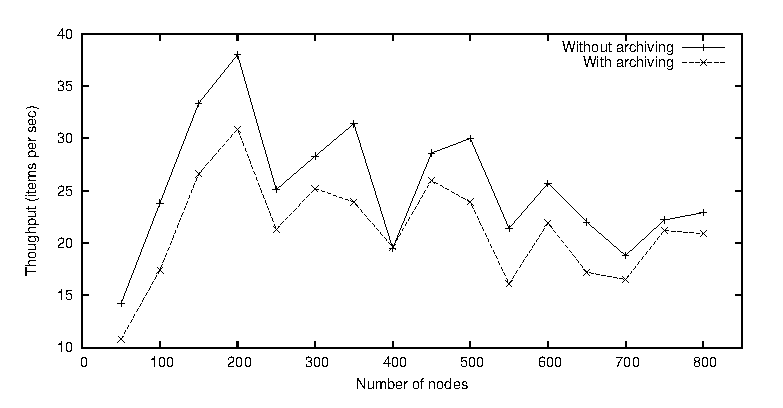
\epsfig{file=throughput.eps, width=\columnwidth}
\caption{Average throughput}
\end{center}
\end{figure}

\begin{figure}
\begin{center}
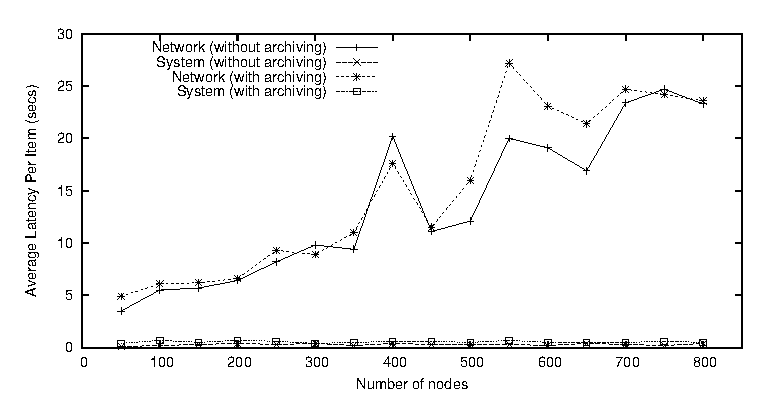
\epsfig{file=latency.eps, width=\columnwidth}
\caption{Average latencies per node}
\end{center}
\end{figure}


\begin{table*}
\begin{center}
\begin{tabular}{|l|r|r|r|r|r|r|r|r|r|r|r|r|}\hline
Num of nodes&	50&	100&	150&	200&	250&	300&	350&	400&	450&	500&	550&	600 \\ \hline\hline
Net latency per node (secs)&	9&	4&	4&	4&	8.6&	5.3&	19.1&	19.5&	14.4&	7.8&	12&	13.3 \\ \hline
Sys latency per node (secs)&	0&	0&	0&	0.3&	0.2&	0.4&	0.3&	0.1&	0.3&	0.4&	0.2&	0.7 \\ \hline
%Total Latency (secs)&	9&	4.04&	4&	4.3&	8.8&	5.8&	19.4&	19.6&	14.7&	8.2&	12.3&	14 \\ \hline
Total fetch time (secs)&	9&	5&	4&	5&	23&	9&	22&	23&	26&	14&	27&	28 \\ \hline	
Throughput (items/sec)&	5.6&	20&	37.5&	40&	10.9&	33.3&	15.9&	17.4&	17.3&	35.7&	20.4&	21.4 \\ \hline
\end{tabular}
\end{center}
\caption{Performance of Comon with no archiving}
\end{table*}


\begin{table*}
\begin{center}
\begin{tabular}{|l|r|r|r|r|r|r|r|r|r|r|r|r|}\hline
Num of nodes&	50&	100&	150&	200&	250&	300&	350&	400&	450&	500&	550&	600 \\ \hline\hline
Net latency per node (secs)&	16&	4&	4&	4&	18.9&	6&	20.6&	22&	8.4&	13&	21.8&	21.3 \\ \hline
Sys latency per node (secs)&	0.8&	1.28&	1.4&	1.8&	1.9&	1.5&	1.6&	1.3&	1.9&	1.7&	1.7&	2.2 \\ \hline
%Total Latency (secs)&	16.8&	5.28&	5.4&	5.8&	20.8&	7.5&	22.2&	23.3&	10.3&	14.7&	23.56&	23.5 \\ \hline
Total fetch time (secs)&	17&	6&	7&	7&	27&	12&	27&	30&	19&	33&	43&	43 \\ \hline
Throughput (items/sec)&	2.9&	16.7&	21.4&	28.6&	9.3&	25&	13&	13.3&	23.7&	15.2&	12.8&	14 \\ \hline
\end{tabular}
\end{center}
\caption{Performance of Comon with archiving}
\end{table*}

\section{A Core Calculus for \forest{}}

\reviewer{I'm hoping extra space can also be used to expand Section 7.
  Is this formal semantics exactly what would would expect from an
  informal intuition of how filesystems work?  Or is the model itself
  a large contribution?  I can imagine re-using this model in a
  mechanical setting (e.g., in Coq) would be useful in certifying the
  lower-levels of the software stack.}

\label{sec:theory}
\newcommand{\us}{\ensuremath{\_\!\_}}
\newcommand{\defeq}{\ensuremath{\triangleq}}
\renewcommand{\bnfdef}{\ensuremath{\mathord{::=}}}
\newcommand{\slsh}{\ensuremath{\mathord{\textsf{/}}}}
\newcommand{\File}[1]{\ensuremath{\mathsf{File}(#1)}}
\newcommand{\Dir}[1]{\ensuremath{\mathsf{Dir}(#1)}}
\newcommand{\Link}[1]{\ensuremath{\mathsf{Link}(#1)}}
\newcommand{\List}[1]{\ensuremath{[ #1 ]}}
\newcommand{\Set}[1]{\ensuremath{\{ #1 \}}}
\newcommand{\Map}[1]{\ensuremath{\{\!\mid #1 \mid\!\}}}
\newcommand{\FAppend}{\ensuremath{\text{++}}}
\newcommand{\FUpdate}[3]{\ensuremath{#1[#2 := #3]}}
\newcommand{\FDelete}[2]{\ensuremath{\FUpdate{F}{r}{\bot}}}
\newcommand{\PNil}{\ensuremath{\bullet}}
\newcommand{\PCons}[2]{\ensuremath{#1\,\textsf{/}\,#2}}
\newcommand{\Just}[1]{\ensuremath{\mathsf{Just(#1)}}}
\newcommand{\Nothing}{\ensuremath{\mathsf{Nothing}}}
\newcommand{\True}{\ensuremath{\mathsf{True}}}
\newcommand{\False}{\ensuremath{\mathsf{False}}}
\newcommand{\fn}[2]{\ensuremath{#1(#2)}}
\newcommand{\Sk}{k^{\tau_m}_{\tau_r}}
%\newcommand{\SAdhoc}[1]{\ensuremath{\mathsf{Adhoc}({#1}^{\tau_m}_{\tau_r})}}
\newcommand{\SAdhoc}[1]{\ensuremath{\mathsf{Adhoc}({#1})}}
\newcommand{\SPred}[1]{\ensuremath{\mathsf{Pred}(#1)}}
\newcommand{\SPath}[2]{\ensuremath{#1\,{::}\,#2}}
\newcommand{\SPair}[3]{\ensuremath{\langle #1 {:} #2, #3 \rangle}}
\newcommand{\SOption}[1]{\ensuremath{(#1)?}}
\newcommand{\SComp}[3]{\ensuremath{[ #1 \mid #2 \in #3 ]}}
\newcommand{\Env}{\ensuremath{\mathcal{E}}}
\newcommand{\ENil}{\ensuremath{\bullet}}
\newcommand{\yields}{\ensuremath{\rightsquigarrow}}
\newcommand{\valid}[1]{\ensuremath{\mathit{valid}(#1)}}
\newcommand{\typ}[1]{\ensuremath{\mathit{#1}}}
\newcommand{\meta}{\typ{att}}
\newcommand{\REP}{\ensuremath{\mathit{REP}}}
\newcommand{\MD}{\ensuremath{\mathit{MD}}}
\newcommand{\md}[1]{\ensuremath{(#1)~\mathit{md}}}
\newcommand{\eval}[3]{\ensuremath{[\![#1]\!]^{#2}_{#3}}}
\newcommand{\pfile}{\ensuremath{\mathsf{File}}}
\newcommand{\pdir}{\ensuremath{\mathsf{Dir}}}
\newcommand{\plink}{\ensuremath{\mathsf{Link}}}
\newcommand{\att}{\ensuremath{\mathsf{a}}}
\newcommand{\defaultatt}{\ensuremath{\att_{\mathsf{default}}}}
\newcommand{\repty}[1]{{\cal R}[\![ #1 ]\!]}
\newcommand{\mdty}[1]{{\cal M}[\![ #1 ]\!]}
\newcommand{\loadkname}[1]{\ensuremath{\mathit{load}_{#1}}}
\newcommand{\storekname}[1]{\ensuremath{\mathit{store}_{#1}}}
\newcommand{\storek}[5]{\fn{\storekname{#1}}{#2,#3,#4,#5}}
\newcommand{\loadk}[4]{\fn{\loadkname{#1}}{#2,#3,#4}}
\newcommand{\stringty}{{string}}
\newcommand{\metapdty}{\meta}
%\newcommand{\load}[5]{#1;#3~\models~#4~~#2~\rhd~(#5) }
%\newcommand{\store}[6]{#1;#3~\models~#5~~(#6)~\lhd~(#2,#4) }
\newcommand{\load}[5]{#1;#3;#4 \vdash #2~\rhd~(#5) }
\newcommand{\store}[6]{#1;#3;#5 \vdash (#6)~\lhd~(#2,#4) }

\begin{figure}
\[
\begin{array}{@{}r@{\,}r@{\,}c@{\,}l}
\textit{Strings}        & n & \in & \Sigma^{\ast} \\[1ex]
\textit{Paths}          & r & \bnfdef & \PNil \mid \PCons{r}{n} \\[1ex]
\textit{Attributes}     & \att  & \bnfdef & \dots\\[1ex]
\textit{Contents}       & T  & \bnfdef & \File{n} \bnfalt \Link{r} \bnfalt \Dir{ \Set{n_1,\dots,n_k} }\\[1ex]
\textit{File sys.}      & F & \bnfdef & \Map{ r_1 \mapsto (\att_1,T_1), \dots, r_k \mapsto (\att_k,T_k) }\\[1ex]
\textit{Values}         & v & \bnfdef & \att \bnfalt n \bnfalt r \bnfalt \True \bnfalt \False \bnfalt () \bnfalt (v_1,v_2) \\
                        &   & \bnfalt & \Just{v} \bnfalt \Nothing \bnfalt \List{v_1,\dots,v_k}\\[1ex]
\textit{Exprs.}         & e & \bnfdef & x \bnfalt v \bnfalt \dots \\[1ex]
\textit{Envs.}          & \Env & \bnfdef & \ENil \bnfalt \Env,x\mapsto v \\[1ex]
\textit{Specs.}         & s & \bnfdef & \Sk 
                              \bnfalt \SPath{e}{s}
                              \bnfalt \SPair{x}{s_1}{s_2} 
                              \bnfalt \SComp{s}{x}{e}
                              \bnfalt \SPred{e}
                              \bnfalt \SOption{s}
\end{array}
\]
\label{fig:calculus-syntax}
\caption{\forest{} calculus syntax}
\end{figure}

\reviewer{... repeatedly refers to Figure 7 when I think it means
  Figure 6.}

\reviewer{In the semantics given for the core calculus, why are
  ML-style types used instead of Haskell-style types?}

This section describes a core calculus that formalizes the essential
features of \forest{} precisely in a simple setting. It is inspired by
classical (\ie{}, not separating, substructural or ambient) unordered
tree logics, customized for file systems. We used this calculus to
investigate various features and prove theorems (such as the
round-tripping properties presented at the end of this section) as we
developed \forest{}.

\subsection{The Basics: File Systems and Their Specifications}

%\paragraph*{File system model.}
%
Figure~\ref{fig:calculus-syntax} presents the formal file system
model. A path $r$ is a sequence of strings\footnote{For simplicity, we
  ignore the special path elements ``..'' and ``.''.  It would be easy
  to add these features, at the cost of complicating the semantics.}
and a file system $F$ is finite map from paths to pairs of attributes
$\att$ and file system contents $T$.  We leave attributes abstract but
expect that they include the usual fields: owner, group, date
modified, {\it etc.}  The attribute $\defaultatt$ contains default
values for all fields. The contents $T$ of a node in the file system
is either a file $\File{n}$ (where $n$ is the string contents of the
file), a symbolic link $\Link{r}$ (where $r$ is the path pointed to by
the link), or a directory $\Dir{\Set{n_1,\dots,n_k}}$ (with paths
$n_1$ to $n_k$). We write $\dom{F}$ for the set of paths $F$ is defined on, 
$F(r)$ for the contents at $r$, and $F(r) = \bot$ when $r$ is not
in $\dom{F}$.

A file system $F$ is {\em well-formed} if it encodes a tree with
directories at the internal nodes and files and symbolic links at the
leaves. More formally, $F$ is well-formed if the following conditions
hold:
%
\begin{itemize}
\item $\dom{F}$ is prefix-closed,
\item $F(r) = (\att,\Dir{ \Set{n_1,\dots,n_k} }) \implies$\\ \hspace*{3.3mm}$\forall i \in \{1,\dots,k\}.~\PCons{r}{n_i} \in \dom{F}$, and
\item $F(r) = (\att,\File{n_r}) \vee F(r) = (\att,\Link{r'}) \implies$\\ \hspace*{3.3mm}$\forall n.~\PCons{r}{n} \not\in \dom{F}$.
\end{itemize}
%
Note that although the structure of a well-formed file system is
tree-shaped, cycles can be also expressed using symbolic links that
point ``upwards'' in the file system.

%\paragraph{File system specifications.}
%
Figure~\ref{fig:calculus-syntax} also presents the syntax of file
system specifications $s$.  We leave the syntax of expression language
abstract but assume that it contains values $v$, variables $x$, and
other operators (of course, in the full \forest{} language,
expressions can be arbitrary Haskell code).  An environment $\Env$
maps variables to values.  The semantic function
$\eval{e}{\Env,r}{\tau}$ evaluates an expression $e$ in the
environment $\Env$ at path $r$, yielding a value $v$ of type $\tau$.

\reviewer{One aspect of the language that I was not clear on is how
  symbolic links work.  Based on the mini-semantics, a symbolic link
  to a directory does not extend the set of valid paths in the file
  system, though a Unix shell, for example, typically treats them that
  way.  How does Forest handle them?}

These file system specifications are parameterized over a collection
of constants $\Sk$, which include specifications for files (\pfile),
directories (\pdir), links (\plink), and \padshaskell{}-described
files (\SAdhoc{b}). The annotations $\tau_r$ and $\tau_m$ supply the
internal types of the the representation and the constant-specific
portion of the meta-data. The meta-variable $b$ ranges over
bidirectional functions: in the forward direction, such functions load
(parse) data; in the reverse direction they store (print) it.

To define the semantics of the overall language precisely,
we assume that each constant is associated with functions
$\loadkname{k}$ and $\storekname{k}$. For example, the $\loadkname{}$
function for the \pfile{} construct, which describes any file (but not
symbolic links or directories), is defined as follows:
%
\[
\loadkname{\pfile}~(\Env,F,r) =
\begin{cases}
  (n,(\True,\att)), \mathrm{if } F(r) = (\att,\File{n}) \\
  (\text{``}{\,}\text{''},(\False,\defaultatt)), \mathrm{otherwise}\\
\end{cases}
\]
%
The arguments to the function include an environment $\Env$, a file system $F$
to load from, and a path $r$ within that file system.
This function either returns the contents and attributes of the file at path $r$,
if it exists, or ``$\,$'' and default attributes if $F$ does not contain a
file at $r$.  The $\storekname{}$ function for \pfile{} is
defined as follows:
%
\[
\begin{array}{l}
\storekname{\pfile}~(\Env,F,r,v,d) =\\[.5ex]
\quad 
\begin{cases}
  (\FUpdate{F}{r}{(\att,\File{v})},            & \text{if}~d = (\True,\att)\\
   \; \phi' = \lambda F'.~ (F'(r) = (\att,\File{v})))\\[1ex]
  \FDelete{F}{r},                              & \text{if}~d = (\False,\att)~\wedge\\
   \; \phi' = \lambda F'.~ F'(r) \neq (\us,\File{\us})) & \;\;\; F(r) = (\us,\File{\us})\\[1ex]
  F,              & \text{otherwise}\\
   \; \phi' = \lambda F'.~ F'(r) \neq (\us,\File{\us}))\\
\end{cases}
\end{array}
\]
%
The arguments to the store function include an environment $\Env$, an
existing file system $F$ to store into, a path $r$ to store at, a
representation $v$ for the data to store, and the metadata $d$ associated
with that representation.  The store function
produces two results: an updated file system $F'$ and a predicate
$\phi'$ that records the constraints needed to ensure
consistency. In this case, the $\storekname{}$ function for \pfile{}
overwrites the contents of the file system $F$ at path $r$ with
$(\att,\File{v})$ if $d$ is valid (and contains $\att$), deletes the
contents of $F$ at $r$ if $d$ is not valid but $F(r)$ contains a file,
and otherwise returns $F$ unchanged. The predicate $\phi'$ requires
that $F'(r)$, the contents of the new file system $F'$ at $r$, be
$\File{v}$ in the first case and that $F'(r)$ not be a file in the other
two cases. These constraints must be satisfied in order to guarantee
the round-tripping properties presented at the end of this section.

\reviewer{For most of the paper, the generation of predicates by the
  store judgment is mysterious and undermotivated.  It would help to
  explain more clearly early on why it's present in the judgment, even
  before the current paragraph explaining the motivation for
  predicates.}

%The load functions for the \plink{} and \pdir{} constants
%are similar. The load function for \SAdhoc{b}{} reads the file system
%in the same way as \pfile{}, but invokes $b$ parser to produce the
%final representation.

In the \forest{} surface syntax, records and paths are specified using
a single construct (and similarly for comprehensions) while the core
calculus models (dependent) records, paths, and comprehensions as
independent, orthogonal constructs.  Path specifications are written
$\SPath{e}{s}$, where $e$ is a path name (to be appended to the
current path) and $s$ specifies a fragment of the file system at that
path. Record specifications are written \SPair{x}{s_1}{s_2}, where $x$
may appear in $s_2$. Comprehension specifications are written
$\SComp{s}{x}{e}$, where $e$ is an expression that describes a set of
values, $x$ is a variable, and $s$, which may depend on $x$, specifies
a fragment of the file system for each value of $x$.  For example, the
specification
\begin{center}
\cd{\{c \kw{is} "c.txt" :: C, d \kw{is} "d.txt" :: D c\}} 
\end{center}
is encoded in the calculus as
%
\(
\SPair{x\,}{\,(\SPath{\texttt{"}\mathtt{c.txt}\texttt{"}}{C})}{(\SPath{\texttt{"}\mathtt{d.txt}\texttt{"}}{D\; x})} 
\).
Similarly, the comprehension
\begin{center}
\cd{[c :: C | c <- \kw{matches} (GL "*")]} 
\end{center}
is encoded as: \(\SPair{x}{\pdir}{\SComp{\SPath{y}{C}}{y}{x}}
\). Predicate specifications $\SPred{e}$ succeed when $e$ evaluates to
\True{} and fail when $e$ evaluates to \False{} under the current
environment.  A \forest{} constraint of the form \cd{s \kw{where} e}
is encoded in the calculus using a dependent pair and a predicate:
$\SPair{x}{s}{\SPred{e[x/\mathtt{this}]}}$. Finally, maybe
specifications are written as $\SOption{s}$ in the calculus.

\begin{figure}
\[
\begin{array}{l|l|l}
s & \repty{s} = & \mdty{s} =  \\
\hline
\Sk & \tau_r &  \tau_m~\mathit{md} \\
\SPath{e}{s} & \repty{s} & \mdty{s} \\
\SPair{x}{s_1}{s_2} & \repty{s_1} \times \repty{s_2} & \md{\mdty{s_1} \times \mdty{s_2}} \\
\SComp{s}{x}{e} & \repty{s}~\typ{list} & \md{\mdty{s}~\typ{list}}    \\
\SPred{e} & \typ{unit} & \typ{unit}~\mathit{md}\\
\SOption{s} & \repty{s}~\typ{option} & \md{\mdty{s}~\typ{option}} %\\
\end{array}
\]
\caption{\forest{} calculus representation and metadata types}
\label{fig:calculus-types}
\end{figure}

\begin{figure*}
\begin{minipage}[t]{.45\textwidth}
\fbox{$\load{\Env}{F}{r}{s}{v,d}$}
\[
\begin{array}{c}
\\[-2.5em]
\infrule
{ }
{ \load{\Env}{F}{r}{\Sk}{ \loadk{k}{\Env}{F}{r} } }
{ }
\\[1.5em]
\infrule
{ \load{\Env}{F}{\eval{\PCons{r}{e}}{\Env,r}{\mathit{path}}}{s}{v,d} }
{ \load{\Env}{F}{r}{\SPath{e}{s}}{v,d} }
{ }
\\[1.5em]
\infrule
{ \begin{array}{c}
  \load{\Env}{F}{r}{s_1}{ v_1,d_1 } \\
  \load{\Env[x \mapsto v_1]}{F}{r}{s_2}{ v_2,d_2 }\\
  b = \valid{d_1} \wedge \valid{d_2}
  \end{array} }
{ \load{\Env}{F}{r}{\SPair{x}{s_1}{s_2}}{ (v_1,v_2),(b, (d_1,d_2)) } }
{ }
\\[1.5em]
\infrule
{ \begin{array}{c}
  \eval{e}{\Env,r}{(\tau\ \mathit{list})} = [w_1,\dots,w_k ]\\
  \forall i \in \{1,\dots,k\}.~\load{\Env[x \mapsto w_i]}{F}{r}{s}{v_i,d_i}\\
  b = \bigwedge_i^k \valid{d_i} \quad \mathit{vs} = [v_1,\dots,v_k] \quad \mathit{ds} = [d_1,\dots,d_k] 
  \end{array} }
{ \load{\Env}{F}{r}{ \SComp{s}{x}{e} }{ \mathit{vs},(b,\mathit{ds}) } }
{ }
\\[1.5em]
\infrule
{ b = \eval{e}{\Env,r}{\mathit{bool}} }
{ \load{\Env}{F}{r}{ \SPred{e} }{ (),(b,()) } }
{ }
\\[1.5em]
\infrule
{ r \not\in \dom{F} }
{ \load{\Env}{F}{r}{ \SOption{s_1} }{ \Nothing,(\False,\Nothing) } }
{ }
\\[1.5em]
\infrule
{ r \in \dom{F} \quad \load{\Env}{F}{r}{s_1}{v_1,d_1} }
{ \load{\Env}{F}{r}{ \SOption{s_1} }{ \Just{v_1},(\valid{d_1},\Just{d_1}) } }
{ }
\end{array}
\]
\end{minipage}\hfill\vrule\hfill\begin{minipage}[t]{.5\textwidth}
\fbox{$\store{\Env}{F}{r}{v,d}{s}{F',\phi'}$}\\
\[
\begin{array}{c}
\\[-2.5em]
\infrule
{ }
{ \store{\Env}{F}{r}{v,d}{\Sk}{ \storek{k}{\Env}{F}{r}{v,d} } }
{ }
\\[1.5em]
\infrule
{ \store{\Env}{F}{\eval{\PCons{r}{e}}{\Env,r}{\mathit{path}}}{v,d}{s}{F',\phi'} }
{ \store{\Env}{F}{r}{v,d}{\SPath{e}{s}}{F',\phi' } }
{ }
\\[1.5em]
\infrule
{ \begin{array}{c}
  \store{\Env}{F}{r}{  v_1,d_1 }{s_1}{ F_1',\phi_1 } \\
  \store{\Env[x \mapsto v_1]}{F}{r}{ v_2,d_2 }{s_2}{ F_2',\phi_2 } \\
  \phi' = \lambda F'.~ (b = \valid{d_1} \wedge \valid{d_2}) \wedge \phi_1'(F') \wedge \phi_2'(F')
  \end{array} }
{ \store{\Env}{F}{r}{ (v_1,v_2),(b,(d_1,d_2)) }{\SPair{x}{s_1}{s_2}}{ F_1' \FAppend F_2',\phi' } }
{ }
\\[1.5em]
\infrule
{ \begin{array}{c}  
  \mathit{vs} = [v_1,\dots,v_j] \quad \mathit{ds} = [d_1,\dots,d_l]\\
  \eval{e}{\Env,r}{(\tau\ \mathit{list})} = [w_1,\dots,w_m ] \quad  k = \min{(j,l,m)} \\
  \forall i \in \{1,\dots,k\}.~\store{\Env[x \mapsto w_i]}{F}{r}{v_i,d_i}{s}{F_i',\phi_i'}\\
  \phi' = \lambda F'.~ (j = l = m) \wedge (b = \bigwedge_i^k \valid{d_i}) \wedge (\bigwedge_i^k \phi_i'(F'))\\
  \end{array} }
{ \store{\Env}{F}{r}{\mathit{vs},(b,\mathit{ds})}{ \SComp{s}{x}{e} }{ F_1' \FAppend \dots \FAppend F_k',\phi' } }
{ }
\\[1.5em]
\infrule
{ \phi' = \lambda F'.~ (b = \eval{e}{\Env,r}{\mathit{bool}}) }
{ \store{\Env}{F}{r}{(),(b,())}{ \SPred{e} }{ F,\phi' } }
{ }
\\[1.5em]
\infrule
{ \begin{array}{c}
  \store{\Env}{F}{r}{ v_1,d_1 }{ s_1 }{ F',\phi_1' }\\
  \phi' = \lambda F'.~ (b = \valid{d_1}) \wedge (r \in \dom{F'}) \wedge \phi_1'(F')
  \end{array} }
{ \store{\Env}{F}{r}{ \Just{v_1},(b,\Just{d_1}) }{ \SOption{s_1} }{ F',\phi' } }
{ }
\\[1.5em]
\infrule
{ \begin{array}{c}
  v = \Nothing \vee d = \Nothing\\
  \phi' = \lambda F'.~ (v = \Nothing) \wedge (d = \Nothing) \wedge \neg b \wedge r \not\in \dom{F'}
  \end{array} }
{ \store{\Env}{F}{r}{ v,(b,d) }{ \SOption{s_1} }{ \FDelete{F'}{r},\phi' } }
{ }
\end{array}
\]
\end{minipage}
\centerline{\hfill (a) \hfill\hfill \hspace*{.05\textwidth} (b) \hfill}
\caption{\forest{} calculus semantics for (a) loading and (b) storing}
\label{fig:calculus-semantics}
\end{figure*}

\reviewer{Why does the second-last rule in the first column return
  "False" as its generic metadata?  Isn't that a signal of an error,
  even though "maybe" formats allow for missing data?}

\subsection{Calculus Semantics}
%
The semantics of the calculus is organized into four separate
definitions, one for each of the four major artifacts generated by the
\forest{} compiler.

\paragraph*{Type Definitions.}
Figure~\ref{fig:calculus-types} defines types for the representations
($\repty{s}$) and metadata ($\mdty{s}$) generated by specifications
$s$. The types for constants $\Sk$ are read off from their annotations
while the types for other specifications are constructed from their
structure in the obvious way---\eg, the type of representations for
\SPair{x}{s_1}{s_2} is a product $(\repty{s_1} \times
\repty{s_2})$. The type constructor $\mathit{md}$ provides a uniform
representation for metadata and is defined as follows:
\[
\begin{array}{lcl}
\tau~\mathit{md} & = & \typ{header} \times \tau \\
\typ{header} & = & \typ{bool} 
\end{array}
\]
The function $\valid{d}$ extracts the boolean from the metadata
structure $d$, returning $\True$ if there are no errors in the
structure and $\False$ otherwise. 

\paragraph*{Semantics of Loading and Storing.}
The inference rules on the left side of
Figure~\ref{fig:calculus-semantics} define the semantics of the load
function. Reading from right to left, the judgment 
$\load{\Env}{F}{r}{s}{v,d}$ states one can obtain the pair $(v,d)$ of
representation and metadata, by materializing components
of the filesystem $F$ in memory using the specification $s$
at path $r$ in environment $\Env$.  Reading from
left to right, this judgment may also be viewed
as a total function from $\Env$, $r$, $s$ and $F$ to $(v,d)$. The
judgment is total because when $F$ fails to match $s$, the load
function generates defaults in the representation $v$ and records
errors in the metadata $d$.  This design allows a programmer to
explore a file system fragment even when it does not match the
given specification exactly.

Let us examine a few of the inference rules that define the store
function in detail. The rule for constants $\Sk$ just invokes the
associated $\storekname{k}$ function. The rule for
$\SComp{s}{x}{e}$ comprehensions is more interesting: it first
evaluates $e$ to a list $[w_1,\dots,w_k]$ and then invokes the store
function for $s$ $k$ times in environments where $x$ is bound to each
$w_i$. It then collects up the results into lists of representations
$[v_1,\dots,v_k]$ and metadata $[d_1,\dots,d_k]$, which it uses as the
final result. The predicate $\SPred{e}$ construct tests whether an
expression $e$ is satisfied. It returns $()$ as the representation and
$(\eval{e}{\Env,r}{\mathit{bool}},())$ as the metadata. Finally,
$\SOption{s}$ invokes $s$'s load function if the current path $r$
exists in the file system, injecting the result into the maybe type
using $\mathsf{Just}$, and otherwise returns $\Nothing$.

The inference rules on the right side of
Figure~\ref{fig:calculus-semantics} define the store function. The
judgment $\store{\Env}{F}{r}{v,d}{s}{F',\phi'}$ states that in
environment $\Env$ storing $(v,d)$ into file system $F$ using
specification $s$ yields the file system $F'$ and predicate
$\phi'$. The predicate $\phi'$ tracks the conditions on the file
system needed to ensure that it accurately reflects the information in
the representation and metadata.

As a simple example to illustrate why predicates are needed, consider
the specification $s = \SPair{x}{\pfile}{\pfile}$ and suppose that the
load function is called in an environment $\Env$ with a file system
$F$ and path $r$ where $F(r) = (\att,\File{n})$. The representation
returned by load will be a pair $(n,n)$ containing two copies of the
file contents at $r$ and the metadata will also contain a pair
$(\True,(\True,\att),(\True,\att)))$ with two copies of the metadata
associated with that file. Now suppose that we change the
representation to $(n,n')$, with $n \neq n'$, and we store the result
back to the file system. Unfortunately, because the representation is
inconsistent---it does not satisfy the dependency between the two
components of the pair implied by $s$---the store function cannot
produce a new file system containing the information in both $n$ and
$n'$. Thus, it must store one and discard the other.  The predicate
$\phi'$ generated by the store function provides a way to track and
report inconsistencies. In this case, the predicate will be equivalent
to the following:
%
\[
\phi' = \lambda F'.~ (F'(r) = (\att,\File{n})) \wedge (F'(r) = (\att,\File{n'})
\]
%
which is obviously not satisfiable when $n \not= n'$. 
\jnf{Say more to
  connect these to manifests?}
\dpw{Thought about it but decided not to. It didn't fit.}

Now that the overall structure of the store judgement has been
explained,
let us examine a few of the inference rules in detail. The rule for
constants $\Sk$ simply invokes the $\storekname{k}$ function. 
The rule for path specifications $\SPath{e}{s}$ passes off
control to the store function for $s$ after replacing the current path
$r$ with $\eval{\PCons{r}{e}}{\Env,r}{\mathit{path}}$. The rule for
dependent pairs $\SPair{x}{s_1}{s_2}$ is more interesting. Given a
pair $(v_1,v_2)$ as the representation, it first invokes the store
function for $s_1$ with $v_1$, producing an updated file system $F_1'$
and predicate $\phi_1'$. Next, it invokes the store function for $s_2$
with $v_2$ in an extended environment where $x$ is bound to $v_1$,
yielding another updated file system $F_2'$ and $\phi_2'$. It combines
the updated file systems using the following right-biased
concatenation operator,
%
\[
\begin{array}{l}
(F_1 \FAppend F_2)(r) = \\
\qquad 
\begin{cases}
  (\att_2,\Dir{N_1 \cup N_2}) & \text{if}~F_1(r) = (\att_1,\Dir{N_1}) \; \wedge \\
                              & \;\;\; F_2(r) = (\att_2,\Dir{N_2})\\
  F_1(r) & \text{if}~F_2(r) = \bot\\
  F_2(r) & \text{otherwise}\\
\end{cases}
\end{array}
\]
%
Finally, it combines the predicates using conjunction. The result is a
file system that contains the consistent changes made to the file
system by the store functions for $s_1$ and $s_2$ as well as a
predicate that checks for the consistency of all of their changes. 

\subsection{Formal Properties}

The first property of the \forest{} calculus is a basic type safety
property, which states that the load function for
specifications $s$ generates representations and metadata belonging to
$\repty{s}$ and $\mdty{s}$ respectively.
%The judgement $\turn v : \tau$ used below is standard; 
%it states that value $v$ has type $\tau$.
%
\begin{proposition}[Type Safety]
  If $\load{\Env}{F}{r}{s}{v,d}$ and $\repty{s} = \tau_{\mathcal{R}}$
  and $\mdty{s} = \tau_{\mathcal{M}}$ then $\turn v :
  \tau_{\mathcal{R}}$ and $\turn d : \tau_{\mathcal{M}}$,
\end{proposition}
%
The above property demonstrates that our type definitions are properly
aligned with the semantics of loading.  To ensure that the semantics
of loading is, in turn, aligned with the semantics of 
storing, we also prove the following two round-tripping
properties.
%

\deferproof{theorem}{loadstore}{LoadStore}{%
  For all environments $\Env$, file systems $F$, paths $r$,
  specifications $s$, representations $v$, and metadata $d$ with
  $\load{\Env}{F}{r}{s}{v,d}$ and
  $\store{\Env}{F}{r}{v,d}{s}{F',\phi}$ we have $F = F'$ and
  $\phi'(F')$.}{%
  The proof is by induction on $s$. We assume that $\loadkname{k}$ and
  $\storekname{k}$ obey the theorem for every constant $\Sk$.
\begin{description}
%%%
%%% CONST
%%%
\item[Case:] $s = \Sk$\\[1ex]
%
By the definitions of the load and store functions we have 
\[ 
\begin{array}{rcl}
v,d  &=& \loadk{k}{\Env}{F}{r}\\
F',\phi' &=& \storek{k}{\Env}{F}{r}{v,d}\\
\end{array}
\]
By assumptions about the behavior of $\loadkname{k}$ and
$\storekname{k}$, we have $F' = F$ and $\phi'(F')$, which finishes
the case.

%%%
%%% PATH
%%%
\item[Case:] $s=\SPath{e}{s_1}$\\[1ex]
%
By the definitions of the load and store functions we have 
\[ 
\begin{array}{l}
\load{\Env}{F}{r'}{s_1}{v,d}\\
\store{\Env}{F}{r'}{v,d}{s_1}{F',\phi'}\\
\end{array} \hspace*{2cm}
\begin{array}{rcl}
r' &=& \eval{\PCons{r}{e}}{\Env,r}{\mathit{path}}\\
\end{array}
\]
By the induction hypothesis applied to $s_1$ we have $F' = F$ and
$\phi'(F')$, which finishes the case.

%%%
%%% Pair
%%%
\item[Case:]$s = \SPair{x}{s_1}{s_2}$:]\\[1ex]
%
By the definitions of the load and store functions we have 
\[ 
\begin{array}{l}
\load{\Env}{F}{r}{s_1}{v_1,d_1}\\
\store{\Env}{F}{r}{v_1,d_1}{s_1}{F_1',\phi_1'}\\
\load{\Env[x \mapsto v_1]}{F}{r}{s_2}{v_2,d_2}\\
\store{\Env[x \mapsto v_1]}{F}{r}{v_2,d_2}{s_2}{F_2',\phi_2'}\\
\end{array} \hspace*{2cm}
\begin{array}{rcl}
b &= & \valid{d_1} \wedge \valid{d_2}\\
v &=& (v_1,v_2)\\
d &=& (b,(d_1,d_2))\\
F' &=& F_1' \FAppend F_2'\\
\phi' &=& \lambda F'.~(b = \valid{d_1} \wedge \valid{d_2}) \wedge \phi_1'(F') \wedge \phi_2'(F')\\
\end{array}
\]
By the induction hypothesis applied to $s_1$, we have $F_1' = F$ and
$\phi_1'(F_1')$. Likewise, by the induction hypothesis applied to
$s_2$, we have $F_2' = F$ and $\phi_2'(F_2')$. We immediately have
$\phi'(F')$ and $F' = F$ as (\FAppend) is idempotent, which finishes
the case.

%%%
%%% Comprehension
%%%
\item[Case:] $s = \SComp{s_1}{x}{e}$\\[1ex]
%
By the definitions of the load and store functions we have 
\[ 
\begin{array}{l}
\eval{e}{\Env,r}{(\tau\ \mathit{list})} = [w_1,\dots,w_k ]\\
\forall i \in \{1,...,k\}.\,\load{\Env[ x \mapsto w_i]}{F}{r}{s_1}{v_i,d_i}\\
\forall i \in \{1,...,k\}.\,\store{\Env[x \mapsto w_i]}{F}{r}{v_i,d_i}{s}{F_i',\phi_i'}\\
\end{array}\hspace*{.75cm}\begin{array}{rcl}
v &=& [v_1,\dots,v_k]\\
b &= &\bigwedge_i^k \valid{d_i}\\
d &=& (b,[d_1,\dots,d_k])\\
F' &=& F_1' \FAppend \dots \FAppend F_k'\\
\phi' &=& \lambda F'.~(k = k = k) \wedge (b = \bigwedge_i^k \valid{d_i}) \wedge (\bigwedge_i^k \phi_i'(F'))\\
\end{array}
\]
By the induction hypothesis applied to $s$ ($k$ times), we have $F_i'
= F$ and $\phi'_i(F_i')$ for $i$ from $1$ to $k$. We immediately have
$\phi'(F')$ and $F' = F$ as (\FAppend) is idempotent, which finishes
the case.

%%%
%%% Predicate
%%%
\item[Case:] $s = \SPred{e}$\\[1ex]
%
By the definition of the load and store functions we have
\[
\begin{array}{rcl}
v &=& ()\\
d &=& (b,())\\
b &=& \eval{e}{\Env,r}{\mathit{bool}}\\
\end{array}\hspace*{2cm}\begin{array}{rcl}
F' &=& F\\
\phi' &=& \lambda F'.~(b = \eval{e}{\Env,r}{\mathit{bool}})\\
\end{array}
\]
Thus, we immediately have $F' = F$ and $\phi'(F')$.

%%%
%%% Option
%%%
\item[Case:] $s = \SOption{s_1}$\\[1ex]
%
We analyze two subcases:
\begin{description}
\item[Subcase:] $r \in \dom{F}$\\[1ex]
%
By the definition of the load and store functions we have
\[ 
\begin{array}{l}
\load{\Env}{F}{r}{s}{v_1,d_1}\\
\store{\Env}{F}{r}{v_1,d_1}{s}{ F',\phi_1' }\\
\end{array}\hspace*{2cm}\begin{array}{rcl}
v &=& \Just{v_1}\\
d &=& (b,\Just{d_1})\\
b &=& \valid{d_1}\\
\phi' &=& \lambda F'.~(b = \valid{d_1}) \wedge (r \in \dom{F}) \wedge \phi_1'(F')\\
\end{array}
\]
%
By the induction hypothesis applied to $s_1$ we have $F' = F$ and
$\phi_1'(F')$. We immediately have $\phi'(F')$.

\item[Subcase:] $r \not\in \dom{F}$\\[1ex]
%
By the definition of the load and store functions we have 
\[ 
\begin{array}{rcl}
v &=& \Nothing\\
d &=& (b,d_1)\\
d_1 &=& \Nothing\\
b &=& \False\\
\end{array}\hspace*{2cm}\begin{array}{rcl}
F' &=& \FDelete{F}{r}\\
\phi' &=& \lambda F'.~(v = \Nothing) \wedge (d_1 = \Nothing) \wedge (\neg b) \wedge  (r \not\in \dom{F'})
\end{array}
\]
We immediately have $F' = F$ and $\phi'(F')$, which finishes the case
and the inductive proof. \hfill \qed
\end{description}
\end{description}
}

\deferproof{theorem}{storeload}{StoreLoad}{ For all environments
  $\Env$, file systems $F$ and $F'$, paths $r$, specifications $s$,
  representations $v$ and $v'$, metadata $d$ and $d'$, and constraints
  $\phi'$ with $\store{\Env}{F}{r}{v,d}{s}{F',\phi'}$ and $\phi'(F')$
  and $\load{\Env}{F'}{r}{s}{v',d'}$ we have $v' = v$ and $\valid{d} =
  \valid{d'}$.}{%
  We will prove a slightly stronger result that implies the theorem:
  for all environments $\Env$, file systems $F$, $G_1$, $G_2$, and
  $F'$, paths $r$, specifications $s$, representations $v$ and $v'$,
  metadata $d$ and $d'$, and constraints $\phi'$ with
  $\store{\Env}{F}{r}{v,d}{s}{F',\phi'}$ and $\phi'(G_1 \FAppend F'
  \FAppend G_2)$ and $\load{\Env}{(G_1 \FAppend F' \FAppend
    G_2)}{r}{s}{v',d'}$ we have $v' = v$ and $\valid{d} =
  \valid{d'}$. The proof is by induction on $s$. We assume that
  $\loadkname{k}$ and $\storekname{k}$ obey the theorem for every
  constant $\Sk$.
\begin{description}
%%%
%%% Constant
%%%
\item[Case]: $s = \Sk$\\[1ex]
%
By the definitions of the load and store functions we have 
\[ 
\begin{array}{rcll}
F',\phi &=& \storek{k}{\Env}{F}{r}{v,d}\\
v',d'  &=& \loadk{k}{\Env}{(G_1 \FAppend F' \FAppend G_2)}{rs}\\
\end{array}
\]
By assumptions about the behavior of $\loadkname{k}$ and
$\storekname{k}$, we have $v' = v$ and $\valid{d} = \valid{d'}$,
which finishes the case. 

%%%
%%% Path
%%%
\item[Case:] $s=\SPath{e}{s_1}$\\[1ex]
%
By the definitions of the load and store functions we have
\[
\begin{array}{l}
\store{\Env}{F}{r'}{v,d}{s_1}{F',\phi'}\\
\load{\Env}{(G_1 \FAppend F' \FAppend G_2)}{r'}{s_1}{v',d'}\\
\end{array}\hspace*{2cm}\begin{array}{rcl}
r' &=& \eval{\PCons{r}{e}}{\Env,r}{\mathit{path}}\\
\end{array}
\]
%
By the induction hypothesis applied to $s_1$ we have $v' = v$ and
$\valid{d} = \valid{d'}$, which finishes the case.

%%%
%%% Pair
%%%
\item[Case:] $s = \SPair{x}{s_1}{s_2}$\\[1ex]
%
By the definition of the load function we have
\[
\begin{array}{l}
\store{\Env}{F}{r}{v_1,d_1}{s_1}{F_1',\phi_1'}\\
\store{\Env[x \mapsto v_1]}{F}{r}{v_2,d_2}{s_2}{F_2',\phi_2'}\\
\end{array}\hspace*{2cm}\begin{array}{rcl}
v &=& (v_1,v_2)\\
d &=& (b,(d_1,d_2))\\
F' &=& F_1' \FAppend F_2'\\
\phi' &=& \lambda F'.~(b = \valid{d_1} \wedge \valid{d_2}) \wedge \phi_1'(F') \wedge \phi_2'(F')\\
\end{array}
\]
By $\phi'(G_1 \FAppend F' \FAppend G_2)$ we have
\[
\begin{array}{l}
b = \valid{d_1} \wedge \valid{d_2}\\
\phi_1'(G_1 \FAppend F' \FAppend G_2)\\
\phi_2'(G_1 \FAppend F' \FAppend G_2)\\
\end{array}
\]
%
As $(\FAppend)$ is associative we also have,
\[
\begin{array}{rcl}
(G_1\FAppend (F_1\FAppend F_2)\FAppend G_2) &=& (G_1\FAppend F_1\FAppend (F_2\FAppend G_2))\\
(G_1\FAppend (F_1\FAppend F_2)\FAppend G_2) &=& ((G_1\FAppend F_1)\FAppend F_2\FAppend G_2),\\
\end{array}
\]
and hence:
\[
\begin{array}{l}
\phi_1'(G_1\FAppend F_1\FAppend (F_2\FAppend G_2))\\
\phi_2'((G_1\FAppend F_1)\FAppend F_2\FAppend G_2)\\
\end{array}
\]
By the definition of the load function we have 
\[ 
\begin{array}{rcll}
\load{\Env}{(G_1 \FAppend F_1 \FAppend (F_2 \FAppend G_2))}{r}{s_1}{v_1',d_1'}\\
\load{\Env[x \mapsto v_1}{((G_1 \FAppend F_1) \FAppend F_2 \FAppend G_2)}{r}{s_2}{v_2',d_2'}\\
\end{array}\hspace*{2cm}\begin{array}{rcl}
v' &=& (v_1',v_2')\\
b' &= & \valid{d_1} \wedge \valid{d_2}\\
d' &=& (b',(d_1',d_2'))\\
\end{array}
\]
%
By the induction hypothesis applied to $s_1$ and $s_2$, we have 
\[
\begin{array}{l}
v_1' = v_1\\
v_2' = v_2\\
\end{array}\hspace*{2cm}\begin{array}{l}
\valid{d_1} = \valid{d_1'}\\
\valid{d_2} = \valid{d_2'}\\
\end{array}
\]
It follows that $(v_1,v_2) = (v_1',v_2')$ and $b = b'$, which
finishes the case.

%%%
%%% Comprehension
%%%
\item[Case:] $s = \SComp{s}{x}{e}$\\[1ex]
By the definition of the store function we have
\[
\begin{array}{l}
\forall i \in \{1,\dots,k\}.\,\store{\Env[x \mapsto w_i]}{F}{r}{v_i,d_i}{s}{F_i',\phi_i}\\
\eval{e}{\Env,r}{(\tau\ \mathit{list})} = [w_1,\dots,w_m ]\\
\end{array}\hspace*{.75cm}\begin{array}{rcl}
v &=& [v_1,\dots,v_j]\\
d &=& [d_1,\dots,d_l]\\
k &=& \min{(j,l,m)}\\
F' &=& F_1' \FAppend \dots \FAppend F_k'\\
\phi &=& \lambda F'.~(j = k = l) \wedge (b = \bigwedge_i^k \valid{d_i}) \bigwedge_i^k \phi_i(F')\\
\end{array}
\]
By $\phi'(G_1 \FAppend F' \FAppend G_2)$ we have
\[
\begin{array}{l}
k = j = l = m\\
b = (\bigwedge_i^k \valid{d_i})\\
\end{array}\hspace*{2cm}\begin{array}{l}
\forall i \in \{1,\dots,k\}.\,\phi_i'(G_1 \FAppend F' \FAppend G_2) \\
\end{array}
\]
%
Let
\[
H_i = ((G_1\FAppend F_1\FAppend \dots \FAppend F_{i-1}) \FAppend F_i \FAppend (F_{i+1} \FAppend \dots \FAppend F_k \FAppend G_2))
\]
for $i$ from $1$ to $k$. As $(\FAppend)$ is associative we have,
\[
(G_1\FAppend (F_1\FAppend \dots \FAppend F_k)\FAppend G_2) = H_i \quad \text{for}~i \in \{1,\dots,k\}
\]
and hence:
\[
\phi_i'(H_i) \quad \text{for}~i \in \{1,\dots,k\}
\]
%
By the definition of the load function we also have 
\[ 
\begin{array}{l}
\forall i \in \{1,\dots,k\}\,\load{\Env[ x \mapsto w_i]}{H_i}{r}{s_1}{v_i,d_i'}\\
\end{array}\hspace*{2cm}\begin{array}{rcl}
v' &=& [v_1',\dots,v_k']\\
b' &=& \bigwedge_i^k \valid{d_i'}\\
d' &=& (b',[d_1',\dots,d_k'])\\
\end{array}
\]
%
By the induction hypothesis applied to $s$ ($k$ times), we have $v_i'
= v_i$ and $\valid{d_i'} = \valid{d_i}$ for = $i$ from $1$ to
$k$. It follows that $[v_1,\dots,v_k] = [v_1',\dots,v_k']$ and $b =
b'$, which finishes the case.

%%%
%%% Predicate
%%%
\item[Case:] $s = \SPred{e}$\\[1ex]
%
By the definitions of the store and load functions we have
\[
\begin{array}{rcl}
v &=& ()\\
d &=& ((),b)\\
F' &=& F\\
\phi' &=& \lambda F'.~(b = \eval{e}{\Env,r}{\mathit{bool}})\\
\end{array}\hspace*{2cm}\begin{array}{rcl}
v' &=& ()\\
d' &=& (b',())\\
b' &=& \eval{e}{\Env,r}{\mathit{bool}}\\
\end{array}
\]
By $\phi'(G_1 \FAppend F' \FAppend G_2)$ we have $b =
\eval{e}{\Env,r}{\mathit{bool}}$. It follows that $v = v'$ and $b =
b'$, which finishes the case.

%%%
%%% Option
%%%
\item[Case:] $s = \SOption{s_1}$\\[1ex]
%
We analyze two subcases:
\begin{description}
\item[Subcase:] $v = \Just{v_1}$ and $d = (b,\Just{d_1})$\\[1ex]
%
By the definition of the store function we have
\[
\begin{array}{l}
\store{\Env}{F}{r}{ v_1,d_1 }{s}{F',\phi_1'}\\
\end{array}\hspace*{2cm}\begin{array}{rcl}
\phi' &=& \lambda F'.~(b = \valid{d_1}) \wedge (r \in \dom{F}) \wedge \phi_1'(F')\\
\end{array}
\]
%
By $\phi'(G_1 \FAppend F' \FAppend G_2)$ we have $b = \valid{d_1}$ and
$r \in \dom{G_1 \FAppend F' \FAppend G_2}$.  By the definition of the
load function we also have
\[ 
\begin{array}{rcll}
\load{\Env}{(G_1 \FAppend F' \FAppend G_2)}{r}{s}{v_1',d_1'}\\
\end{array}\hspace*{2cm}\begin{array}{rcl}
v' &=& \Just{v_1'}\\
b' &=& \valid{d_1'}\\
d' &=& (b',\Just{d_1'})\\
\end{array}
\]
By the induction hypothesis applied to $s_1$ we have $v_1' = v_1$ and
$b' = b$. It follows that $v' = v$.

\item[Subcase:] $r \not\in \dom{F}$\\[1ex]
%
By the definition of the store and load functions we have
\[
\begin{array}{rcl}
F' &=& \FDelete{F}{r}\\
\phi' &=& \lambda F'.~(v = \Nothing) \wedge (d = \Nothing) \wedge (\neg b) \wedge (r \not\in \dom{F'})\\
\end{array}\hspace*{2cm}\begin{array}{rcl}
v' &=& \Nothing\\
b' &=& \False\\
d' &=& (b',\Nothing)\\
\end{array}
\]
As $\phi'(G_1 \FAppend F' \FAppend G_2)$ we have $v = \Nothing$ and $d
= \Nothing$ and $\neg b$ and $r \not\in \dom{G_1 \FAppend F' \FAppend
  G_2}$. Thus, we immediately have $v' = v$ and $b' = b$, which finishes the case and
the inductive proof. \hfill \qed
\end{description}
\end{description}}

\smallskip

\noindent The first theorem states that loading from a file system $F$
and immediately storing the resulting representation and metadata
yields the original file system and, moreover, it satisfies the
predicate produced by the store function. The second theorem states
that storing an arbitrary representation and metadata and then loading
the resulting file system yields the same representation and contains
errors only if the original metadata also contained errors. These
properties are based on the general correctness conditions that have
been proposed for bidirectional transformations in the context of
lenses~\cite{lenses}, but are generalized here to accommodate the
inconsistencies that can arise when working with imperfect, ad hoc
data. The proofs of these theorems can be found in
Appendix~\ref{sec:proof-appendix}. 


\section{Related Work}\label{sec:related}


\section{Conclusions}
\label{sec:conclusion}


\section*{Acknowledgments}

We wish to thank Simon Peyton Jones for extending Haskell's
quasiquoting mechanism to support the \forest{} design and for
assisting us in its use. We also wish to thank John Launchbury for
helping us design and implement Pads/Haskell.

This work was supported in part by the NSF under grant CCF-1016937,
the ONR under grant N00014-09-1-0652, and the NSFC under grant
6103302. Any opinions, findings, and recommendations expressed in this
material are those of the authors and do not necessarily reflect the
views of these agencies.

\bibliographystyle{abbrv}
\balance
\bibliography{pads}

\ifappendix
\newpage
\appendix
\onecolumn

% JNF: TeX hackery for deferring proofs :-)
\closeproofchan
\section{Proofs}

\noindent This appendix contains the proofs of the theorems stated in
Section~\ref{sec:theory}.

\label{sec:proof-appendix}
\input{proof-appendix}

\newpage
%\documentclass[fleqn]{article}
\documentclass[nocopyrightspace,natbib,onecolumn,9pt]{sigplanconf}
%\documentclass[nocopyrightspace]{sigplanconf}

\newif\ifdraft\drafttrue  %% set to false in final version

\usepackage{xspace,pads,amsmath,math-cmds,
            math-envs,inference-rules,times,
            verbatim,alltt,multicol,proof,url}
\usepackage{epsfig}
\usepackage{code} 
\usepackage{color}
\usepackage{tikz}
%\setlength{\oddsidemargin}{0in}
%\setlength{\evensidemargin}{0in}
%\setlength{\textwidth}{6.5in}
%\setlength{\textheight}{8.5in}

\begin{document}
\newcommand{\cut}[1]{}
\newcommand{\reminder}[1]{{\it #1 }}
\newcommand{\edcom}[1]{\textbf{{#1}}}
\newcommand{\poplversion}[1]{#1}
\newcommand{\trversion}[1]{}

\newcommand{\appref}[1]{Appendix~\ref{#1}}
\newcommand{\secref}[1]{Section~\ref{#1}}
\newcommand{\tblref}[1]{Table~\ref{#1}}
\newcommand{\figref}[1]{Figure~\ref{#1}}
\newcommand{\listingref}[1]{Listing~\ref{#1}}
%\newcommand{\pref}[1]{{page~\pageref{#1}}}

\newcommand{\eg}{{\em e.g.}}
\newcommand{\cf}{{\em cf.}}
\newcommand{\ie}{{\em i.e.}}
\newcommand{\etal}{{\em et al}}
\newcommand{\etc}{{\em etc.\/}}
\newcommand{\naive}{na\"{\i}ve}
\newcommand{\role}{r\^{o}le}
\newcommand{\forte}{{fort\'{e}\/}}
\newcommand{\appr}{\~{}}

\newcommand{\bftt}[1]{{\ttfamily\bfseries{}#1}}
\newcommand{\kw}[1]{\bftt{#1}}
\newcommand{\pads}{\textsc{pads}}
\newcommand{\padsc}{\textsc{pads/c}}
\newcommand{\padx}{\textsc{padx}}
\newcommand{\ipads}{\textsc{ipads}}
\newcommand{\ir}{\textsc{IR}}
\newcommand{\padsl}{\textsc{padsl}}
\newcommand{\padsml}{\textsc{pads/ml}}
%\newcommand{\padsd}{\textsc{pads/d}}
\newcommand{\learnpads}{{\textsc{learnpads}}}
\newcommand{\padsd}{\textsc{Gloves}}
\newcommand{\blt}{\textsc{blt}}
\newcommand{\ddc}{\textsc{ddc}}
\newcommand{\ddl}{\textsc{ddl}}
\newcommand{\C}{\textsc{C}}
\newcommand{\perl}{\textsc{Perl}}
\newcommand{\ml}{\textsc{ml}}
\newcommand{\smlnj}{\textsc{sml/nj}}
\newcommand{\ocaml}{\textsc{OCaml}\xspace}
\newcommand{\haskell}{\textsc{haskell}\xspace}
\newcommand{\ocamlbig}{\textsc{OCAML}\xspace}
\newcommand{\java}{\textsc{java}}
\newcommand{\xml}{\textsc{xml}}
\newcommand{\html}{\textsc{html}}
\newcommand{\xpath}{\textsc{xpath}}
\newcommand{\xquery}{\textsc{xquery}}
\newcommand{\datascript}{\textsc{datascript}}
\newcommand{\packettypes}{\textsc{packettypes}}
\newcommand{\erlang}{\textsc{Erlang}}
\newcommand{\camlp}{\cd{Camlp4}}
\newcommand{\ocamlnet}{\cd{Ocamlnet} \cd{2}}

\newcommand{\totalcost}[2]{\textsc{Cost}(#1,#2)}
\newcommand{\costdescription}[1]{\textsc{CT}(#1)}
\newcommand{\normcostdescription}{\textsc{NCT}}
\newcommand{\costdata}[2]{\textsc{CD}(#2 \; | \; #1)}
\newcommand{\acostdata}[2]{\textsc{ACD}(#2 \; | \; #1)}
\newcommand{\adc}[2]{\textsc{CD'}(#2 \; | \; #1)}
\newcommand{\cardt}{\textsc{Card}}
\newcommand{\costvar}[1]{\textsc{CV}(#1)}
\newcommand{\costchar}[1]{\textsc{CA}(#1)}
\newcommand{\coststring}[1]{\textsc{CS}(#1)}
\newcommand{\costint}[1]{\textsc{CI}(#1)}
\newcommand{\costparam}[1]{\textsc{CP}(#1)}
\newcommand{\costconst}[1]{\textsc{CC}(#1)}

\newcommand{\dibbler}{Sirius}
\newcommand{\ningaui}{Altair}
\newcommand{\darkstar}{Regulus}

\newcommand{\vizGems}{Arrakis}

\newcommand{\comon}{CoMon\xspace}
\newcommand{\planetlab}{PlanetLab\xspace}
\newcommand{\monall}{Monall\xspace}
%% \newcommand{}{}


%% \newcommand{\IParray}[4]{{\tt Parray} \; #1 \; \[#2, #3, #4\]}

\newcommand{\figHeight}[4]{\begin{figure}[tb]
	\centerline{
	            \epsfig{file=#1,height=#4}}
	\caption{#2}
	\label{#3}
	\end{figure}}

\newcommand{\myalt}{\ensuremath{\; | \;}}
\newcommand{\normal}[1]{\ensuremath{\bar{#1}}}
\newcommand{\relativee}[2]{\ensuremath{{\cal R}(#1 \; || \; #2)}}
\newcommand{\srelativee}[2]{\ensuremath{{\cal S}(#1 \; || \; #2)}}
\newcommand{\addh}[2]{\ensuremath{#1 \oplus #2}}

\newcommand{\irstruct}[1]{{\tt struct}\{#1\}}
\newcommand{\irunion}[1]{{\tt union}\{#1\}}
\newcommand{\irenum}[1]{{\tt enum}\{#1\}}
\newcommand{\irarray}[1]{{\tt array}\{#1\}}
\newcommand{\irarrayFW}[2]{{\tt arrayFW}\{#1\}[#2]}
\newcommand{\irswitch}[2]{{\tt switch}(#1)\{#2\}}
\newcommand{\iroption}[1]{{\tt option}\{#1\}}
\newcommand{\setof}[1]{\lsem #1 \rsem}
\newcommand{\goto}{\Rightarrow}
\newcommand{\Pvoid}{{\tt Pvoid}}
\newcommand{\Pempty}{{\tt Pempty}}
\newcommand{\sskip}{\hspace*{5mm}}
\newcommand{\shrink}{\vspace*{-4mm}}

% Semantics
\newcommand{\setalt}{{\; | \;}}
\newcommand{\denote}[1]{\lsem #1 \rsem}
\newcommand{\lsem}{{[\![}}
\newcommand{\rsem}{{]\!]}}
\newcommand{\turn}{\vdash}
\newcommand{\meta}{m}
\newcommand{\nested}{n}
\newcommand{\mytime}[1]{#1.t}
\newcommand{\myds}[1]{#1.ds}
\newcommand{\myval}[1]{#1.nest}
\newcommand{\generatedloc}{\ensuremath{\mathtt{nowhere}}}
\newcommand{\environment}{E}
\newcommand{\universe}{U}
\newcommand{\selectOne}{\ensuremath{\mathsf{earliest}}}
% core feed semantics
\newcommand{\csemantics}[3]{{\cal C}\lsem #1 \rsem_{{#2} \, {#3}}}
% feed semantics
\newcommand{\semantics}[3]{{\cal F}\lsem #1 \rsem_{{#2} \, {#3}}}
% expression semantics
\newcommand{\esemantics}[2]{{\cal E}\lsem #1 \rsem_{{#2}}}
%\newcommand{\esemantics}[2]{#2(#1)}

% Host language types
\newcommand{\ty}{\ensuremath{\tau}}
\newcommand{\basety}{\ensuremath{b}}
\newcommand{\arrow}{\rightarrow}
\newcommand{\optionty}[1]{\ensuremath{#1 \; \mathsf{option}}}
\newcommand{\listty}[1]{\ensuremath{#1 \; \mathsf{list}}}
\newcommand{\setty}[1]{\ensuremath{#1 \; \mathsf{set}}}
\newcommand{\feedty}[1]{\ensuremath{#1 \; \mathsf{feed}}}
\newcommand{\corety}[1]{\ensuremath{#1 \; \mathsf{core}}}
\newcommand{\schedulety}{\ensuremath{\mathsf{sched}}}
\newcommand{\timety}{\ensuremath{\mathsf{time}}}
\newcommand{\locty}{\ensuremath{\mathsf{loc}}}
\newcommand{\boolty}{\ensuremath{\mathsf{bool}}}
\newcommand{\unitty}{\ensuremath{\mathsf{unit}}}
\newcommand{\stringty}{\ensuremath{\mathsf{string}}}
\newcommand{\metatype}[1]{\ensuremath{\mathsf{meta}(#1)}}
\newcommand{\nestedtype}[1]{\ensuremath{\mathsf{nest}(#1)}}
\newcommand{\dsty}{\ensuremath{\mathsf{ds}}}

\newcommand{\dom}{\ensuremath{\mathsf{dom}}}
\newcommand{\ueq}[3]{\ensuremath{#1 =_{#2} #3}}
\newcommand{\fsubset}[3]{\ensuremath{#1 \subseteq_{#2} #3}}
\newcommand{\feq}[3]{\ensuremath{#1 =_{#2} #3}}

% Expressions
\newcommand{\expression}{e}
\newcommand{\constant}{c}
\newcommand{\ds}{\ensuremath{ds}}
\newcommand{\boolf}{\ensuremath{\mathtt{false}}}
\newcommand{\boolt}{\ensuremath{\mathtt{true}}}
\newcommand{\loc}{\ensuremath{\ell}}
\newcommand{\feed}{\ensuremath{F}}
\newcommand{\corefeed}{\ensuremath{C}}
\newcommand{\generalvar}{\ensuremath{x}}
\newcommand{\feedvar}{\ensuremath{x}}
\newcommand{\itemvar}{\ensuremath{x}}
\newcommand{\data}{\ensuremath{v}}
\newcommand{\atime}{\ensuremath{t}}
\newcommand{\astring}{\ensuremath{w}}
\newcommand{\unit}{\ensuremath{()}}
\newcommand{\schedule}{\ensuremath{s}}
\newcommand{\parser}{\ensuremath{p}}
\newcommand{\none}{\ensuremath{\mathtt{None}}}
\newcommand{\some}[1]{\ensuremath{\mathtt{Some}\; #1}}
\newcommand{\inl}[1]{\ensuremath{\mathtt{inl}\; #1}}
\newcommand{\inr}[1]{\ensuremath{\mathtt{inr}\; #1}}
\newcommand{\casedata}[2]{{\tt switch}(#1)\{#2\}}
%\newcommand{\nillist}{\ensuremath{\mathtt{nil}}}
\newcommand{\nillist}{\ensuremath{[\,]}}
%\newcommand{\conslist}[2]{\ensuremath{\mathtt{cons} (#1,#2)}}
\newcommand{\conslist}[2]{\ensuremath{[#1,\ldots,#2]}}
\newcommand{\nilstream}{\ensuremath{\mathtt{done}}}
\newcommand{\consstream}[2]{\ensuremath{\mathtt{next} (#1,#2)}}


% Feeds
\newcommand{\comprehensionfeed}[3]{\ensuremath{\mathtt{\{|} #1 \; \mathtt{|}\; #2 \leftarrow #3 \mathtt{|\}}}}
\newcommand{\computed}[3]{\ensuremath{\mathtt{[} #1 \; \mathtt{|}\; #2 \in #3 \mathtt{]}}}
\newcommand{\letfeed}[3]{\ensuremath{\mathtt{let}\; #1 \; \mathtt{=}\; #2 \; \mathtt{in} \; #3}}
\newcommand{\allfeed}[5]{
  \ensuremath{
    \mathtt{all \{ format=} #1; 
    \mathtt{src=} #2;
    \mathtt{sched=} #3;
    \mathtt{pp=} #4;
    \mathtt{win=} #5;
  \mathtt{\}}}}
\newcommand{\existsfeed}[5]{
  \ensuremath{
    \mathtt{any \{ format=} #1; 
    \mathtt{src=} #2;
    \mathtt{sched=} #3;
    \mathtt{pp=} #4;
    \mathtt{win=} #5;
  \mathtt{\}}}}
\newcommand{\filterfeed}[2]{
  \ensuremath{
    \mathtt{filter} \; #1 \; \mathtt{with}\; #2}}
\newcommand{\remapfeed}[2]{
  \ensuremath{
    \mathtt{redirect} \; #1 \; \mathtt{with}\; #2}}
\newcommand{\ppfeed}[2]{
  \ensuremath{
    \mathtt{pp} \; #1 \; \mathtt{with}\; #2}}
\newcommand{\foreachupdate}[3]{
  \ensuremath{
    \mathtt{foreach{*}{*}}\; #1 \;
    \mathtt{in}\; #2 \;
    \mathtt{update}\; #3}}
\newcommand{\foreachcreate}[3]{
  \ensuremath{
    \mathtt{foreach*}\; #1 \;
    \mathtt{in}\; #2 \;
    \mathtt{create}\; #3}}
\newcommand{\remap}[2]{\ensuremath{\mathtt{redirect}\; #1 \; \mathtt{with} \; #2}}
\newcommand{\stutterfeed}[2]{\ensuremath{\mathtt{stutter}\; #1 \; \mathtt{on} \; #2}}
\newcommand{\refeed}[2]{\ensuremath{\mathtt{reschedule}\; #1 \; \mathtt{to} \; #2}}
\newcommand{\emptyfeed}{\ensuremath{\emptyset}}
\newcommand{\onefeed}[2]{\ensuremath{\mathtt{One}}(#1,#2)}
\newcommand{\sfeed}[1]{\ensuremath{\mathtt{SchedF}}(#1)}
\newcommand{\lfeed}[1]{\ensuremath{\mathtt{ListF}}(#1)}
\newcommand{\unionfeed}{\ensuremath{\cup}}
\newcommand{\sumfeed}{\ensuremath{+}}
\newcommand{\spairfeed}{\; \ensuremath{\mathtt{\&} \; }}
\newcommand{\allpairfeed}{\; \ensuremath{{*}{*}} \; }

\newcommand{\Time}{\ensuremath{\mathtt{Time}}}
\newcommand{\Set}{\ensuremath{\mathtt{Set}}}

% this is used for the translations equal
\newcommand{\transeq}{\stackrel{def}{=} }
\newcommand{\ai}{{\tt wl}}



% BNF
%\newcommand{\bnfalt}{\ |\ }


\conferenceinfo{PLDI'11,}{} 
\copyrightyear{2011} 
\copyrightdata{} 

\title{Forest: A Language and Toolkit For Programming with \Filestores{}}

\authorinfo{Auxiliary Materials for PLDI Review}
	   {\vskip -.5in}
           {}

\cut{
\authorinfo{Kathleen Fisher}
	   {AT\&T Labs Research}
           {\mono{kfisher@research.att.com}}
\authorinfo{Nate Foster}
           {Cornell University}
           {\mono{jnfoster@cs.cornell.edu}}
\authorinfo{David Walker}
           {Princeton University}
           {\mono{{dpw}@CS.Princeton.EDU}}
}

\maketitle{}


\section{Introduction}
This document contains auxiliary materials provided for the PLDI 2011
review process. Specifically, it contains \forest{} descriptions of a
variety of different \filestores{}.

Please note that this document is best viewed electronically.  Some of
the graphs generated are very large, but shrunk down to fit on a
single page.  They will not display well when
printed.  However, reviewers may zoom in electronically
on the PDF to view the details.


\section{Pads Web Site Descripton}
This \forest{} description describes the \pads{} web site. The
description starts with \pads{} descriptions of files that contain
information that impacts the directory structure. The
configuration file supplies the paths where various components of the
website should be located.  The \cd{SourceNames} file lists the names
of the data files available for the demo.  Each user directory will
have a subdirectory for each file listed in \cd{SourceNames}. Each
user is logged in the file \cd{UserEntries}.  For each user in this
file, there is a directory with a corresponding name containing all of
the information relevent to that user.  A graph
of the \pads{} website, generated using the \cd{ForestGraph} tool
follows the description.
\begin{code}
\mkred{\{-# LANGUAGE TypeSynonymInstances, TemplateHaskell, QuasiQuotes,
    MultiParamTypeClasses, FlexibleInstances, DeriveDataTypeable,
    ScopedTypeVariables #-\}} 
\mbox{}
\kw{module} Examples.PWS \kw{where}
\kw{import} Language.Pads.Padsc
\kw{import} Language.Forest.Forestc \kw{hiding} (sources)
\kw{import} System.IO.Unsafe (unsafePerformIO)
\kw{import} Language.Pads.GenPretty
\kw{import} Language.Forest.Graph
\mbox{}
[pads| 
  \mkred{-- Configuration file for learning demo web site; contains paths to various web site components.}
  \kw{data} Config_f =  Config_f \{
                      header      :: [Line StringLn] \kw{length} 13,
   "$host_name   =",  host_name   :: Config_entry_t,  \mkred{-- Name of machine hosting web site}
   "$static_path =",  static_path :: Config_entry_t,  \mkred{-- URL prefix for static content}
   "$cgi_path    =",  cgi_path    :: Config_entry_t,  \mkred{-- URL prefix for cgi content}
   "$script_path =",  script_path :: Config_entry_t,  \mkred{-- Path to directory of scripts in live web site}
   "$tmp_root    =",  tmp_root    :: Config_entry_t,  \mkred{-- Path to directory for demo user data}
   "$pads_home   =",  pads_home   :: Config_entry_t,  \mkred{-- Path to directory containing pads system}
   "$learn_home  =",  learn_home  :: Config_entry_t,  \mkred{-- Path to directory containing learning system}
   "$sml_home    =",  sml_home    :: Config_entry_t,  \mkred{-- Path to directory containing SML executable}
   "$install_src =",  install_src :: Config_entry_t,  \mkred{-- Path to directory containing learning demo website source}
   "$static_dst  =",  static_dst  :: Config_entry_t,  \mkred{-- Path to directory for static content in live web site}
   "$cgi_dst     =",  cgi_dst     :: Config_entry_t,  \mkred{-- Path to directory for cgi content in live web site site}
                      trailer     :: [Line StringLn]
   \}
\mbox{}
  \kw{type} Config_entry_t = Line (" \\"",  StringC '\\"',  "\\";")   
\mbox{}
  \kw{newtype} Header_t = Header_t ([Line StringLn] \kw{length} 13)
\mbox{}
  \mkred{\{- File listing data sources for web site -\}}
  \kw{newtype} SourceNames_f = SourceNames_f [Line StringLn]
\mbox{}
  \mkred{\{- Information related to a single user's use of the web site -\}}
  \kw{newtype} UserEntries_f = UserEntries_f ([Line UserEntry_t] \kw{terminator} EOR)
\mbox{}
  \mkred{\{- Each visitor gets assigned a userId that is passed as a ? parameter in URL.
     Security considerations preclude using user-modifiable values as part of file paths.
     Thus, we map each userId to a corresponding dirId.
     The dirId names the directory containing the associated user's data. 
     A userEntry_t contains a single such mapping.
     A file with type userEntries_t describes a collection of such mappings.
  -\}}
  \kw{data} UserEntry_t =  UserEntry_t \{
     "id.",   usrId :: Int,               
    ",id.",   dirId :: (Int, '.', Int)    \kw{where} <| usrId == fst dirId |> 
  \} 
\mbox{}
  \mkred{\{- Log of requests.  Used to prevent denial of service attacks. -\}}
  \kw{newtype} LogFile_f = LogFile_f [Line LogEntry_t]
\mbox{}
\end{code}

\begin{code}

  \mkred{\{- Request entry.  -\}}
  \kw{data} LogEntry_t = LogEntry_t \{
    userId :: Int,         ',',   \mkred{-- user making request}
    ip     :: IP_t,        ',',   \mkred{-- IP address of requestor}
    script :: StringC ' ', ' ',   \mkred{-- script to be executed}
    userDir:: StringC ' ', ' ',   \mkred{-- directory to put results, corresponds to user}
    padsv  :: StringC ' ', ' ',   \mkred{-- version of PADS used}
    sml    :: StringSE '[ ]',     \mkred{-- version of SML used}
    msg    :: Maybe StringLn      \mkred{-- optional message}
  \}
\mbox{}
  \kw{type} IP_t = (Int, '.', Int, '.', Int, '.', Int)
|]
\end{code}

\begin{code}


\mbox{}
[forest|
  \mkred{\{- Files with various permission settings. -\}}
  \kw{type} BinaryRO    = BinaryFile    \kw{where} <| get_modes this_att ==  "-rw-r--r--" |>
  \kw{type} BinaryRX    = BinaryFile    \kw{where} <| get_modes this_att ==  "-rwxr-xr-x" |>
  \kw{type} TextRX      = TextFile      \kw{where} <| get_modes this_att ==  "-rwxr-xr-x" |>
  \kw{type} TextRO      = TextFile      \kw{where} <| get_modes this_att ==  "-rw-r--r--" |>
\mbox{}  
  \mkred{\{- Optional binary file with read/execute permission. -\}}
  \kw{type} OptBinaryRX = Maybe BinaryRX
\mbox{}
  \mkred{\{- Files with PADS descriptions -\}}
  \kw{type} Config      = File Config_f      \kw{where} <| get_modes this_att ==  "-rw-r--r--" |>
  \kw{type} SourceNames = File SourceNames_f \kw{where} <| isReadOnly this_att |>
  \kw{type} UserEntries = File UserEntries_f \kw{where} <| isReadOnly this_att |>
  \kw{type} LogFile     = File LogFile_f     \kw{where} <| isReadOnly this_att |>
\mbox{}
  \mkred{\{- Directory of image files -\}}
  \kw{type} Imgs_d = \kw{Directory} \{
    logo     \kw{is} "pads_small.jpg" :: BinaryRO,
    favicon  \kw{is} "favicon.ico"    :: BinaryRO
  \}
\mbox{}
  \mkred{\{- Directory of static content -\}}
  \kw{type} Static_d = \kw{Directory} \{
    style_sheet \kw{is} "pads.css"           :: TextRO,   
    intro_redir \kw{is} "learning-demo.html" :: TextRO,   
    title_frame \kw{is} "atitle.html"        :: TextRO,   
    logo_frame  \kw{is} "top-left.html"      :: TextRO,   
    top_frame   \kw{is} "banner.html"        :: TextRO,   
    empty_frame \kw{is} "nothing.html"       :: TextRO,
    images      \kw{is} "images"             :: Imgs_d \kw{where} <| get_modes images_md == "drwxr-xr-x" |>
  \}
\mbox{}
\mkred{\{- Directory of dynamic content -\}}
  \kw{type} Cgi_d = \kw{Directory} \{
    config'       \kw{is} "PLConfig.pm"             :: TextRO,   
    perl_utils    \kw{is} "PLUtilities.pm"          :: TextRO,     
    intro         \kw{is} "learning-demo.cgi"       :: TextRX,     
    intro_nav     \kw{is} "navbar-orig.cgi"         :: TextRX,     
    select_data   \kw{is} "pads.cgi"                :: TextRX,     
    result_nav    \kw{is} "navbar.cgi"              :: TextRX,     
    format_chosen \kw{is} "data-results.cgi"        :: TextRX,     
    gen_desc      \kw{is} "build-description.cgi"   :: TextRX,     
    get_user_data \kw{is} "build-roll-your-own.cgi" :: TextRX,     
    gen_desc_usr  \kw{is} "genData.cgi"             :: TextRX,     
    build_lib     \kw{is} "build-library.cgi"       :: TextRX,     
    build_accum   \kw{is} "build-accum.cgi"         :: TextRX,     
    build_xml     \kw{is} "build-xml.cgi"           :: TextRX,     
    build_fmt     \kw{is} "build-fmt.cgi"           :: TextRX     
  \}

\end{code}

\begin{code}
\mkred{\{- Directory of shell scripts invoked by CGI to run learning system -\}}
 \kw{type} Scripts_d = \kw{Directory} \{
    rlearn                    :: TextRX,    \mkred{-- Shell script for running PADS comiler on stock format}
    rlearnown \kw{is} "rlearn-own" :: TextRX,    \mkred{-- Shell script for running PADS compiler on user format}
    raccum    \kw{is} "r-accum"    :: TextRX,    \mkred{-- Shell script to generate and run accumulator}
    rxml      \kw{is} "r-xml"      :: TextRX,    \mkred{-- Shell script to generate and run XML converter}
    rfmt      \kw{is} "r-fmt"      :: TextRX,    \mkred{-- Shell script to generate and run formating program}
    rlibrary                  :: TextRX     \mkred{-- Shell script to build PADS library}
  \}
\mbox{}
\mkred{\{- Directory containing administrative files used by demo web site -\}}
 \kw{type} Info_d = \kw{Directory} \{
     sources \kw{is} "sampleFiles" :: SourceNames,  \mkred{-- List of source data files whose formats can be learned}
     users   \kw{is} "userFile"    :: UserEntries,  \mkred{-- Mapping from userIDs to associated directory names}
     logFile \kw{is} "logFile"     :: LogFile       \mkred{-- Log of server actions.}
  \}                          
\mbox{}
\mkred{\{- Collection of files named by sources containing actual data.  -\}}
 \kw{type} DataSource_d(sources :: [String]) =  [ s :: TextFile | s <- sources ]
\mbox{}
\mkred{\{- Type of a symbolic link with pointing to source-\}}
 \kw{type} SymLink_f (path :: FilePath) = SymLink \kw{where} <| this == path |>
\mbox{}
\mkred{\{- Directory of optional links to source data files -\}}
 \kw{type} Data_d ((root,sources) :: (FilePath, [String])) = \kw{Directory} {
     datareps  \kw{is} [s :: Maybe TextFile                        | s <- sources],
     datalinks \kw{is} [s :: Maybe (SymLink_f <| root++"/"++ s |>) | s <- sources]        
 }
\mbox{}
\mkred{\{- Directory that stores the generated machine-dependent output for data source named source -\}}
 \kw{type} MachineDep_d (source :: String) = \kw{Directory} \{
   pads_c    \kw{is} <| source ++ ".c"    |> :: TextRO,      \mkred{-- Generated C source for PADS description}
   pads_h    \kw{is} <| source ++ ".h"    |> :: TextRO,      \mkred{-- Generated C header for PADS description}
   pads_o    \kw{is} <| source ++ ".o"    |> :: BinaryRO,    \mkred{-- Compiled library for PADS description}
   pads_pxml \kw{is} <| source ++ ".pxml" |> :: TextRO,      \mkred{-- PADS description in xml syntax}
   pads_xsd  \kw{is} <| source ++ ".xsd"  |> :: TextRO,      \mkred{-- Xschema of XML syntax for source description}
   pads_acc  \kw{is} <| source ++ "-accum"|> :: OptBinaryRX, \mkred{-- Optional generated accumulator program}
   pads_fmt  \kw{is} <| source ++ "-fmt"  |> :: OptBinaryRX, \mkred{-- Optional generated formatting program}
   pads_xml  \kw{is} <| source ++ "-xml"  |> :: OptBinaryRX  \mkred{-- Optional generated XML conversion program}
 \}

\mbox{}
\mkred{\{- Directory that stores the generated output for data source named "source". -\}}
 \kw{type} Example_d (source :: String) = \kw{Directory} \{
   pads_p         \kw{is} <| source ++ ".p" |>            :: TextRO,         \mkred{-- PADS/C description of data source}
   pads_pml       \kw{is} <| source ++ ".pml" |>          :: Maybe TextRO,   \mkred{-- PADS/ML description of data source}
   vanilla        \kw{is} "vanilla.p"                     :: TextRO,         \mkred{-- input tokenization}
   makefile       \kw{is} "GNUmakefile"                   :: TextFile,       \mkred{-- Makefile}
   machine        \kw{is} <| envVar "AST_ARCH"|>          :: Maybe (MachineDep_d source),   \mkred{-- Platform dependent files}
   accum_c        \kw{is} <| source ++ "-accum.c" |>      :: Maybe TextRO,   \mkred{-- Template for accumulator program}
   accum_out      \kw{is} <| source ++ "-accum.out"|>     :: Maybe TextRO,   \mkred{-- ASCII Accumulator output}
   accum_xml_out  \kw{is} <| source ++ "-accum_xml.out"|> :: Maybe TextRO,   \mkred{-- XML Accumulator output}
   xml_c          \kw{is} <| source ++ "-xml.c"|>         :: Maybe TextRO,   \mkred{-- Template for XML converter}
   xml_out        \kw{is} <| source ++ "-xml.out"|>       :: Maybe TextRO,   \mkred{-- XML representation of source}
   xml_xsd        \kw{is} <| source ++ ".xsd" |>          :: Maybe TextRO,   \mkred{-- Xschema for XML representation of source}
   fmt_c          \kw{is} <| source ++ "-fmt.c" |>        :: Maybe TextRO,   \mkred{-- Template for formatting program}
   fmt_out        \kw{is} <| source ++ "-fmt.out" |>      :: Maybe TextRO    \mkred{-- Formatted representation of source}
 \}
\mbox{}
\mkred{\{- Directory that stores all information for one user. -\}}
 \kw{type} User_d(arg@ (r, sources) :: (FilePath, [String])) = \kw{Directory} \{
    dataSets    \kw{is} "data"    :: Maybe (Data_d arg),
    runExamples \kw{is}       [ s :: Maybe (Example_d s) | s <- sources]
  \}
\mbox{}
\mkred{\{- Collection of directories containing temporary information for all users. -\}}
 \kw{type} Users_d((r,info) :: (FilePath, Info_d)) = 
    [userDir :: User_d <|(r, getSources info) |>  | userDir <- <| userNames info |> ]
\mbox{}
\end{code}

\begin{code}
\mkred{\{- Top-level of PADS website. -\}}
 \kw{type} Website_d(config::FilePath)  = \kw{Directory} \{
  c               \kw{is} config               :: Config,           \mkred{-- Locations of other components}
  static_content  \kw{is} <| gstatic_dst c  |> :: Static_d,         \mkred{-- Static web site content}
  dynamic_content \kw{is} <| gcgi_dst c     |> :: Cgi_d,            \mkred{-- Dynamic web site content}
  scripts         \kw{is} <| gscript_path c |> :: Scripts_d,        \mkred{-- Shell scripts to run learning system}
  admin_info      \kw{is} <| gstatic_dst c  |> :: Info_d,           \mkred{-- Administrative information about website}
  data_dir        \kw{is} <| (glearn_home c)++"/examples/data" |>
                  :: DataSource_d <|(getSources admin_info)|>, \mkred{-- Stock data files for website}
  usr_data        \kw{is} <| gtmp_root c |>    :: Users_d  <|(get_fullpath data_dir_md, admin_info)|>   
                                                               \mkred{-- User-specific information}
 \}
 
|]
\mbox{}
\mkred{\{- HASKELL HELPER FUNCTIONS -\}}
isReadOnly md = get_modes md == "-rw-r--r--"
\mbox{}
\mkred{\{- Function userName gets the list of user directorn names from an info structure. -\}}
userNames info = getUserEntries (users info)
getUserEntries (UserEntries (UserEntries_f users)) = map userEntryToFileName users
userEntryToFileName userEntry = pairToFileName (dirId userEntry)
pairToFileName (n1, n2) = "id."++(show n1)++"."++(show n2)
\mbox{}
\mkred{\{- Helper functiosn to convert a Config entry to a FileName -\}}
ghost_name   (Config c) = host_name c
gstatic_path (Config c) = static_path c
gcgi_path    (Config c) = cgi_path c
gscript_path (Config c) = script_path c
glearn_home  (Config c) = learn_home c
gtmp_root    (Config c) = tmp_root c
gstatic_dst  (Config c) = static_dst c
gcgi_dst     (Config c) = cgi_dst c


\end{code}
\newpage
%\begin{figure}
%\vskip -.25in
\begin{center}
\scalebox{.13}{
\includegraphics{website.pdf}}
\end{center}
%\caption{Graph showing structure of PADS website, generated from
%  description using \texttt{ForestGraph}}
%\label{fig:pws}
%\end{figure}
\newpage
\section{Students.hs Description}
This section includes the \forest{} description of the Princeton
Computer Science Department \filestore{}.
The following is the initial portion of a student record, shown here
to illustrate the format.
\begin{code}
KESSEL, PHIL	   BSE   '11
- - - - - - - - - - - - - - - - - - -
Type    Yr  Course     Grade
         1             A+ to F
d        2             P  (  Pass )
t  D  p  3             INC
o  .  .  4  Dept  xxx  N  (Not Avail)
- - - - - - - - - - - - - - - - - - -
d  .  .  1  COS   101  C
o  .  .  1  HOC   101  A
o  .  .  1  GOL   599  A+
...
\end{code}

\begin{code}
\textcolor{red}{-- Auxiliary Haskell functions for PADS description}
ws   = RE "[ \t]+"
ows  = RE "[ \t]*"
junk = RE ".*"
space = ' '
quote = '\''
comma = ','
\end{code}

\begin{code}
\textcolor{red}{-- PADS description of Princeton CS Student Record Format}
[pads| 
  \kw{type} Grade = Pre "[ABCD][+-]?|F|AUD|N|INC|P"
\mbox{}
  \kw{data} Course = 
    \{ sort         :: Pre "[dto]",           ws
    , departmental :: Pre "[.D]",            ws
    , passfail     :: Pre "[.p]",            ws
    , level        :: Pre "[1234]",          ws
    , department   :: Pre "[A-Z][A-Z][A-Z]", ws
    , number       :: Pint \kw{where} <| 100 <= number && number < 600 |>, ws
    , grade        :: Grade,                 junk                               
    \} 
\mbox{}
  \kw{data} Middle_name = \{space, middle :: Pre "[a-zA-Z]+[.]?" \}    
\mbox{} 
  \kw{data} Student_Name(myname::String) = 
    \{ lastname   :: Pre "[a-zA-Z]*"  \kw{where} <| toString lastname ==  myname |>,  comma, ows     
    , firstname  :: Pre "[a-zA-Z]*" 
    , middlename :: Maybe Middle_name
    \}
\mbox{}
  \kw{data} School = AB | BSE
\mbox{}
  \kw{data} Person (myname::String) =
    \{ fullname   :: Student_Name myname,    ws
    , school     :: School,                 ws, quote
    , year       :: Pre "[0-9][0-9]"
    \}
\mbox{}
  \kw{type} Header  = [Line (Pre ".*")] \kw{with} term length of 7 
  \kw{type} Trailer = [Line (Pre ".*")] \kw{with} term Eof 
  \kw{data} Student (name::String) = 
    \{ person  :: Line (Person name)
    , Header  
    , courses :: [Line Course]
    , Trailer
    \}
|]
\end{code}

\begin{code}
\textcolor{red}{-- Auxiliary Haskell functions for Forest description}
template s = s `elem` ["SSSS.txt", "SSS.txt", "sxx.txt", "sss.txt", "ssss.txt"]
not_template = not . template
\mbox{}
getYear :: String -> Integer
getYear s = read (reverse (take 2 (reverse s)))
toStrN i n = (replicate  (n - length (show i)) '0') ++ (show i)
mkClass y = "classof" ++ (toStrN y 2)
\mbox{}
transferRE  = RE "TRANSFER|Transfer"
leaveRE     = RE "LEAVE|Leave"
withdrawnRE = RE "WITHDRAWN|WITHDRAWAL|Withdrawn|Withdrawal|WITHDREW"
cRE         = RE "classof[0-9][0-9]" 
txt         = GL "*.txt"
\end{code}


\begin{code}
\textcolor{red}{-- FOREST description of Princeton CS Department Database}
[forest|
  \textcolor{red}{-- Root of the hierarchy}
  \kw{type} PrincetonCS (y::Integer) = \kw{Directory}
    \{ notes \kw{is} "README" :: Text
    , seniors   \kw{is} <|mkClass y      |> :: Class y
    , juniors   \kw{is} <|mkClass (y + 1)|> :: Class <| y + 1 |>
    , graduates :: Grads
    \}
\mbox{}
  \textcolor{red}{-- Collection of directories containing graduated students}
  \kw{type} Grads = 
     Map [ c :: Class <| getYear c |> | c <- matches cRE ] 
\mbox{}
  \textcolor{red}{-- Directory containing all students in a particular year}
  \kw{type} Class (y :: Integer) = \kw{Directory}
    \{ bse \kw{is} <|"BSE" ++ (toStrN y 2)|> :: Major
    , ab  \kw{is} <|"AB"  ++ (toStrN y 2)|> :: Major   
    , transfer  \kw{matches} transferRE  :: Maybe Major 
    , withdrawn \kw{matches} withdrawnRE :: Maybe Major 
    , leave     \kw{matches} leaveRE     :: Maybe Major 
    \}
\mbox{}
  \textcolor{red}{-- Collection of files containing all students in a particular major.}
  \kw{type} Major = Map 
    [ s :: File (Student <| dropExtension s |>) 
    | s <- \kw{matches} txt,  <| (not . template) s |>  ]  
|]
\end{code}
\vfill{}

\subsection{Generated Description}

Here follows a description generated from a small sample of the
student directory data using the description inference tool.

%\begin{figure}
\begin{code}
\kw{data} transfer = \kw{Directory} \{
\}

\kw{data} wITHDREW = \kw{Directory} \{
    fingertxt \kw{is} "finger.txt" :: File Ptext
\}

\kw{data} tRANSFER = \kw{Directory} \{
    bEAUCHEMINtxt \kw{is} "BEAUCHEMIN.txt" :: File Ptext,
    vERSTEEGtxt \kw{is} "VERSTEEG.txt" :: File Ptext
\}

\kw{data} bSE11 = \kw{Directory} \{
    transfer \kw{is} "transfer" :: transfer,
    bOZAKtxt \kw{is} "BOZAK.txt" :: File Ptext,
    kESSELtxt \kw{is} "KESSEL.txt" :: File Ptext,
    ssstxt \kw{is} "sss.txt" :: File Ptext
\}

\kw{data} aB11 = \kw{Directory} \{
    kADRItxt \kw{is} "KADRI.txt" :: File Ptext,
    mACARTHERtxt \kw{is} "MACARTHER.txt" :: File Ptext,
    oRRtxt \kw{is} "ORR.txt" :: File Ptext,
    sSSStxt \kw{is} "SSSS.txt" :: File Ptext
\}

\kw{data} classof11 = Directory \{
    aB11 \kw{is} "AB11" :: aB11,
    bSE11 \kw{is} "BSE11" :: bSE11,
    tRANSFER \kw{is} "TRANSFER" :: tRANSFER,
    wITHDREW \kw{is} "WITHDREW" :: wITHDREW
\}
\end{code}
%\caption{Generated description. Type \texttt{File Ptext} is synonymous
%  with \texttt{Text}.}
%\label{fig:generated-description}
%\end{figure}
%\vfill

\newpage

\section{Coral.hs Description}

This section gives the PADS and Forest descriptions for the CoralCDN
Log repository. A graph of the CoralCDN
repository, generated like the graph above using the \cd{ForestGraph}
tool from the description and (a subset of) the actual repository 
follows.


\begin{code}
\textcolor{red}{-- Auxiliary Haskell definitions for PADS description}
comma\_ws  = REd ",[ \t]*" " "
status\_re = REd "[0-9]+" "0"
\mbox{}
\textcolor{red}{-- PADS description of CoralCDN Webserver Log Format}
[pads|
  \kw{type} Time = (Int, ".", Int)
\mbox{}
  \kw{type} Byte = \kw{constrain} x :: Int \kw{where} <| 0 <= x && x <= 256 |>
\mbox{}
  \kw{data} IP\_Port = IP\_Port
    \{ '"', 
      ip :: (Byte,'.',Byte,'.',Byte,'.', Byte), ":",
      port :: Int, '"' \}
\mbox{}
  \kw{type} Status = StringME status\_re
\mbox{}
  \kw{data} Statistics = Statistics
    \{ stats\_size       :: Int,              comma\_ws
    , stats\_proxy      :: StringME '[01]',  comma\_ws
    , stats\_level      :: Int,              comma\_ws
    , stats\_lookup     :: Int,              comma\_ws
    , stats\_xfer       :: Int,              comma\_ws
    , stats\_total      :: Int \}
\mbox{}
  \kw{type} NoQuote = StringME '[^\\"]*'
\mbox{}
  \kw{type} Generic = ('"',NoQuote,'"')
\mbox{}
  \kw{type} Url = Generic
\mbox{}
  \kw{data} Header = Header
    \{ version       :: Maybe (StringME '[12],[ \\t]*')
    , time          :: Time     \}
\mbox{}
  \kw{data} Request = Request
   \{ src       :: IP\_Port, comma\_ws
   , dst       :: IP\_Port, comma\_ws
   , url       :: Url \} 
\mbox{}
  \kw{data} InData = InData
    \{ "\\"IN\\"",               comma\_ws
    , in\_req     :: Request,  comma\_ws
    , in\_status1 :: Status,   comma\_ws
    , in\_status2 :: Status,   comma\_ws
    , in\_stats   :: Statistics \}
\mbox{}
  \kw{data} OutData = OutData
    \{ "\\"OUT\\"",                            comma\_ws 
    , out\_remote    :: StringME <| RE "\\"(REM|LOC)\\"" |> , comma\_ws
    , out\_req       :: Request,             comma\_ws
    , out\_referrer  :: Url,                 comma\_ws
    , out\_status    :: Status,              comma\_ws
    , out\_stats     :: Statistics,          comma\_ws
    , out\_forwarded :: Generic,             comma\_ws
    , out\_via       :: Generic  \}
\mbox{}
  \kw{data} InOut = In InData | Out OutData
\mbox{}
  \kw{data} Entry = Entry
    \{ header  :: Header,   comma\_ws
    , payload :: InOut
    , Eor \}
\mbox{}
  \kw{type} Entries = [Entry] \kw{terminator} EOR
\mbox{}  
  \kw{data} Coral = Coral (Entries, EOF)
|]
\end{code}

\begin{code}
\textcolor{red}{-- Forest description of CoralCDN Log Repository}
[forest|
  \textcolor{red}{-- Directory containing log files}
  \kw{type} Log = \kw{Directory}
    \{ web \kw{is} "coralwebsrv.log.gz" :: Gzip (File Coral),          
      dns \kw{is} "coraldnssrv.log.gz" :: Maybe (Gzip TextFile),
      prb \kw{is} "probed.log.gz"      :: Maybe (Gzip TextFile),
      dmn \kw{is} "corald.log.gz"      :: Maybe (Gzip TextFile) \}
\mbox{}
  \textcolor{red}{-- Directory containing dates}
  \kw{type} Site = [ d :: Log | d <- \kw{matches} <| RE "[0-9]\{4\}\_[0-9]\{2\}\_[0-9]\{2\}-[0-9]\{2\}\_[0-9]\{2\}" |> ] 
\mbox{}
  \textcolor{red}{-- Directory containing sites}
  \kw{type} Top = [ s :: Site | s <- \kw{matches} <| RE "[^.].*" |> ] 
|]
\end{code}

\begin{code}

\textcolor{red}{-- Load function for CoralCDN description}
(rep,md) = unsafePerformIO \$ top\_load "/var/log/coral"
\mbox{}
\textcolor{red}{-- Helpers: deconstruct representations }
get\_sites :: Top -> [(String,Site)]
get\_dates :: Site -> [(String,Log)]
get\_entries :: Log -> [Entry]
\mbox{}
\textcolor{red}{-- Helpers: project fields }
get\_stats :: Entry -> Statistics
get\_total :: Entry -> Int
get\_date :: String -> String 
get\_url::Entry -> String
string\_of\_url :: Url -> String

\textcolor{red}{-- Helpers: test if entry is for incoming our outgoing
  data}
is\_in  :: Entry -> Bool
is\_out :: Entry -> Bool
\mbox{}
\textcolor{red}{-- Helper: builds an association list }
lmap f p tdir = 
   [ f host datetime e | (host,hdir) <- get\_sites tdir,
                         (datetime,ldir) <- get\_dates hdir,
                          e <- get\_entries ldir,
                          p e ]
\mbox{}
\textcolor{red}{-- Uses of lmap}
by\_date = lmap ({\char92}h d e -> (get\_date d, get\_total e))
by\_host = lmap ({\char92}h d e -> (h, get\_total e))
by\_url\_bytes = lmap ({\char92}h d e -> (get\_url e, get\_total e))
by\_url\_counts = lmap ({\char92}h d e -> (get\_url e, 1))

\mbox{}
\textcolor{red}{-- Helpers: fold down an association list}
go\_bins m p = fromListWith (+) (m p rep)
\mbox{}
count\_bins m = fromListWith (+) (fold ({\char92} c l -> (c,1):l) [] m)
\mbox{}
go\_flat p = 
  sum [ (get\_total e) | (host,hdir) <- get\_sites tdir,
                        (datetime,ldir) <- get\_dates hdir,
                        e <- get\_entries ldir,
                        p e ]
\mbox{}
\textcolor{red}{-- Several useful queries }
in\_total = go\_flat is\_in
out\_total = go\_flat is\_out
in\_by\_host = go\_bins by\_host is\_in
out\_by\_host = go\_bins by\_host is\_out 
in\_by\_date = go\_bins by\_date is\_in 
out\_by\_date = go\_bins by\_date is\_out
in\_url\_bytes = go\_bins by\_url\_bytes is\_in
out\_url\_bytes = go\_bins by\_url\_bytes is\_out
in\_url\_counts = go\_bins by\_url\_counts is\_in
out\_url\_counts = go\_bins by\_url\_counts is\_out
in\_counts\_urls = count\_bins \$ go\_bins by\_url\_counts is\_in
out\_counts\_urls = count\_bins \$ go\_bins by\_url\_counts is\_out
num\_sites () = case load\_logs () of Top l -> List.length l
\mbox{}
\textcolor{red}{-- Top-k URLs } 
topk k = 
  take k \$ sortBy sortDown \$ toList \$
  fromListWith (+)
    [ (get\_url e, get\_total e)
    | (site,sdir) <- get\_sites rep,
      (datetime,ldir) <- get\_dates sdir,
      e <- get\_entries ldir,
      is\_in e ]
\end{code}


%\begin{figure}
\begin{center}
\centerline{\noindent\tikz\node[scale=.7]{\pgfimage{Coral}};}
\end{center}
%\caption{Graph showing structure of the CoralCND log repository,
%  generated from the description using \texttt{ForestGraph}}
%\label{fig:coral}
%\end{figure}









\newpage

\section{Gene Ontology}

This section presents a description of gene ontology data found 
here: \url{http://www.geneontology.org/gene-associations/}.
Once again, a graph generated using \texttt{ForestGraph}
on a subset of the data follows the description.
%Graph showing structure of a small subset of the Gene Ontology \filestore, generated from 
%  the description using 

\begin{code}
\mkred{-- PADS descriptions of data file format.}
[pads|
  \kw{type} Pfloat         = (Pint, '.', Pint)
  \kw{type} Pdate          = \{mon :: Pint, '/', day :: Pint, '/', year :: Pint\}
  \kw{type} Purl           = ("http://", Pstringln)
  \kw{type} Version_t      = ("!CVS Version: Revision: ", Pfloat, ws, '$')
  \kw{type} Valid_date_t   = ("!GOC Validation Date: ", Pdate, ws, '$')
  \kw{type} Sub_date_t     = ("!Submission Date: ", Pdate)
  \kw{type} Project_name_t = ("!Project_name: ", Pstringln)
  \kw{type} URL_t          = ("!URL: ", Purl)
  \kw{type} Email_t        = ("!Contact Email: ", Pstringln)
  \kw{type} Funding_t      = ("!Funding: ", Pstringln)
  \kw{type} Gaf_ver_t      = ("!gaf-version: ", Pfloat)
  \kw{type} Organism_t     = ("!organism:", ws, Pstringln)
  \kw{type} Date_t         = ("date:", ws, Pdate)
  \kw{type} Note_t         = ('!', ws, Pstringln)
\mbox{} 
  \kw{data} Header_line_t = 
	Version Version_t
	| Valid_date Valid_date_t
	| Sub_date Sub_date_t
	| Project_name Project_name_t
	| URL URL_t
	| Email Email_t
	| Funding Funding_t
	| Gaf_ver Gaf_ver_t
	| Organism Organism_t
	| Date Date_t
	| Note Note_t
	| Other ('!', Pstringln)
\mbox{} 
  \kw{type} Other_line_t = Pstringln
\mbox{} 
  \kw{type} GA_f = ([Line Header_line_t], [Line Other_line_t] \kw{with} term Eof)
|]
\mbox{} 
[pads|
  \kw{data} Pair_t = \{key::Pstring '=', '=', val::Pstringln\}
  \kw{type} Conf_f = [Line Pair_t] \kw{with} term Eof 
|]
\mbox{} 
[pads|
  \kw{type} Xml_header = ("<?xml ", Pstringln)
  \kw{type} XML_f = (Line Xml_header, [Line Pstringln])
|]
\end{code}

\begin{code}
\mkred{-- Forest description of Gene Ontology \filestore{}}
[forest|
  \kw{type} Readme_d = \kw{Directory} \{
    readmes \kw{is} [rm :: Maybe Text | rm <- <|map get_readme_file (comb_source sources)|>]
  \}
\mbox{}
  \kw{type} PTHR_d (name :: String)  = \kw{Directory} \{
   attr  \kw{is}  <| name ++ ".save.attr"  |> :: Text,
   gaf   \kw{is}  <| name ++ ".save.gaf"   |> :: Text,
   msa   \kw{is}  <| name ++ ".save.msa"   |> :: Text,
   paint \kw{is}  <| name ++ ".save.paint" |> :: File XML_f,
   sfan  \kw{is}  <| name ++ ".save.sfan"  |> :: Text,
   tree  \kw{is}  <| name ++ ".save.tree"  |> :: Text,
   txt   \kw{is}  <| name ++ ".save.txt"   |> :: Text, 
   wts   \kw{is}  <| name ++ ".save.txt"   |> :: Text
  \}
\mbox{}
  \kw{type} Pre_sub_d = \kw{Directory} \{
    pre_gz_files   \kw{is} [gz   :: Maybe (Gzip (File GA_f)) | gz   <- <|map get_gz_file   (comb_source sources)|>],
    pre_conf_files \kw{is} [conf :: Maybe (File Conf_f)      | conf <- <|map get_conf_file (comb_source sources)|>]
  \}
\mbox{}
  \kw{type} Paint_d = \kw{Directory} \{
    pthr_dirs \kw{is} [dir_name :: PTHR_d (dir_name) | dir_name <- \kw{matches} RE "PTHR[0-9]+"],
    pre_sub   \kw{is} "pre-submission" :: Pre_sub_d
  \}
\mbox{}
  \kw{type} Submission_d = \kw{Directory} \{
    gz_files    \kw{is} [gz   :: Maybe (Gzip (File GA_f)) | gz   <- <|map get_gz_file   (comb_source sources)|>],
    conf_files  \kw{is} [conf :: Maybe (File Conf_f)      | conf <- <|map get_conf_file (comb_source sources)|>],
    paint_files \kw{is} [cs   :: Maybe (File Conf_f) 
                        | cs <- <|map (\\x -> get_conf_file ("paint" ++ x)) (comb_source sources)|>], 
    paint_d     \kw{is} "paint"               :: Paint_d
  \}
\mbox{}
  \kw{type} Top_d = \kw{Directory} \{
    data_files \kw{is} [gz :: Maybe (Gzip (File GA_f)) | 
			gz <- <|map get_gz_file (comb_source sources)|>],
    readme     \kw{is} "readme"             :: Readme_d,
    sub        \kw{is} "submission"         :: Submission_d
  \}
|]
\mbox{}
\mkred{-- Haskell code to generate graph corresponding to sample data set in \filestore{} "Data/ga"}
doImg = \kw{do}
 { (rep,md) <- top_d_load "Data/ga"
 ; mdToPDF md "Examples/ga.pdf"
 }
\end{code}

\begin{code}
\mkred{-- Auxiliary Haskell Definitions}
ws = RE "[ \t]+"
title = "gene_association"
get_gz_file f = title ++ "." ++ f ++ ".gz"
get_readme_file f = f ++ ".README"
get_conf_file f = title ++ "."  ++ f ++ ".conf"
\mbox{}
\mkred{\{- each source is a pair (institute name, list of organisms the institute provides) -\}}
sources = [
	  ("Compugen", [])
	, ("GeneDB", ["Lmajor","Pfalciparum","Spombe","Tbrucei","tsetse"])
	, ("PAMGO", ["Atumefaciens","Ddadantii","Mgrisea","Oomycetes"])
	, ("aspgd", [])
	, ("cgd", [])
	, ("dictyBase", [])
	, ("ecocyc", [])
	, ("fb", [])
	, ("goa", ["arabidopsis","chicken","cow","human","mouse","pdb","rat",
                   "uniprot","uniprot_noiea","zebrafish"])
	, ("gramene", ["oryza"])
	, ("jcvi", ["Aphagocytophilum","Banthracis","Cburnetii","Chydrogenoformans",
                    "Cjejuni","Cperfringens","Cpsychrerythraea","Dethenogenes","Echaffeensis",
                    "Gsulfurreducens","Hneptunium","Lmonocytogenes","Mcapsulatus","Nsennetsu",
                    "Pfluorescens","Psyringae","phaseolicola","Soneidensis","Spomeroyi",
		    "Vcholerae"])
	, ("mgi", [])
	, ("pseudocap", [])
	, ("reactome", [])
	, ("rgd", [])
	, ("sgd", [])
	, ("sgn", [])
	, ("tair", [])
	, ("wb", [])
	, ("zfin", []) ]


comb_source [] = []
comb_source ((inst, organs):sources) = 
   \kw{let} cl = \kw{case} organs \kw{of}
	  [] -> [inst]
	  _ -> map (\\organism -> inst ++ "_" ++ organism) organs
   in cl ++ (comb_source sources) 

\mkred{
\{- the GO files, when unzipped, contain a header like the following:
!CVS Version: Revision: 1.19 $
!GOC Validation Date: 01/27/2007 $
!Submission Date: 1/15/2007
-\}
}
\end{code}

\begin{figure}
\vskip -.25in
\begin{center}
\scalebox{.35}{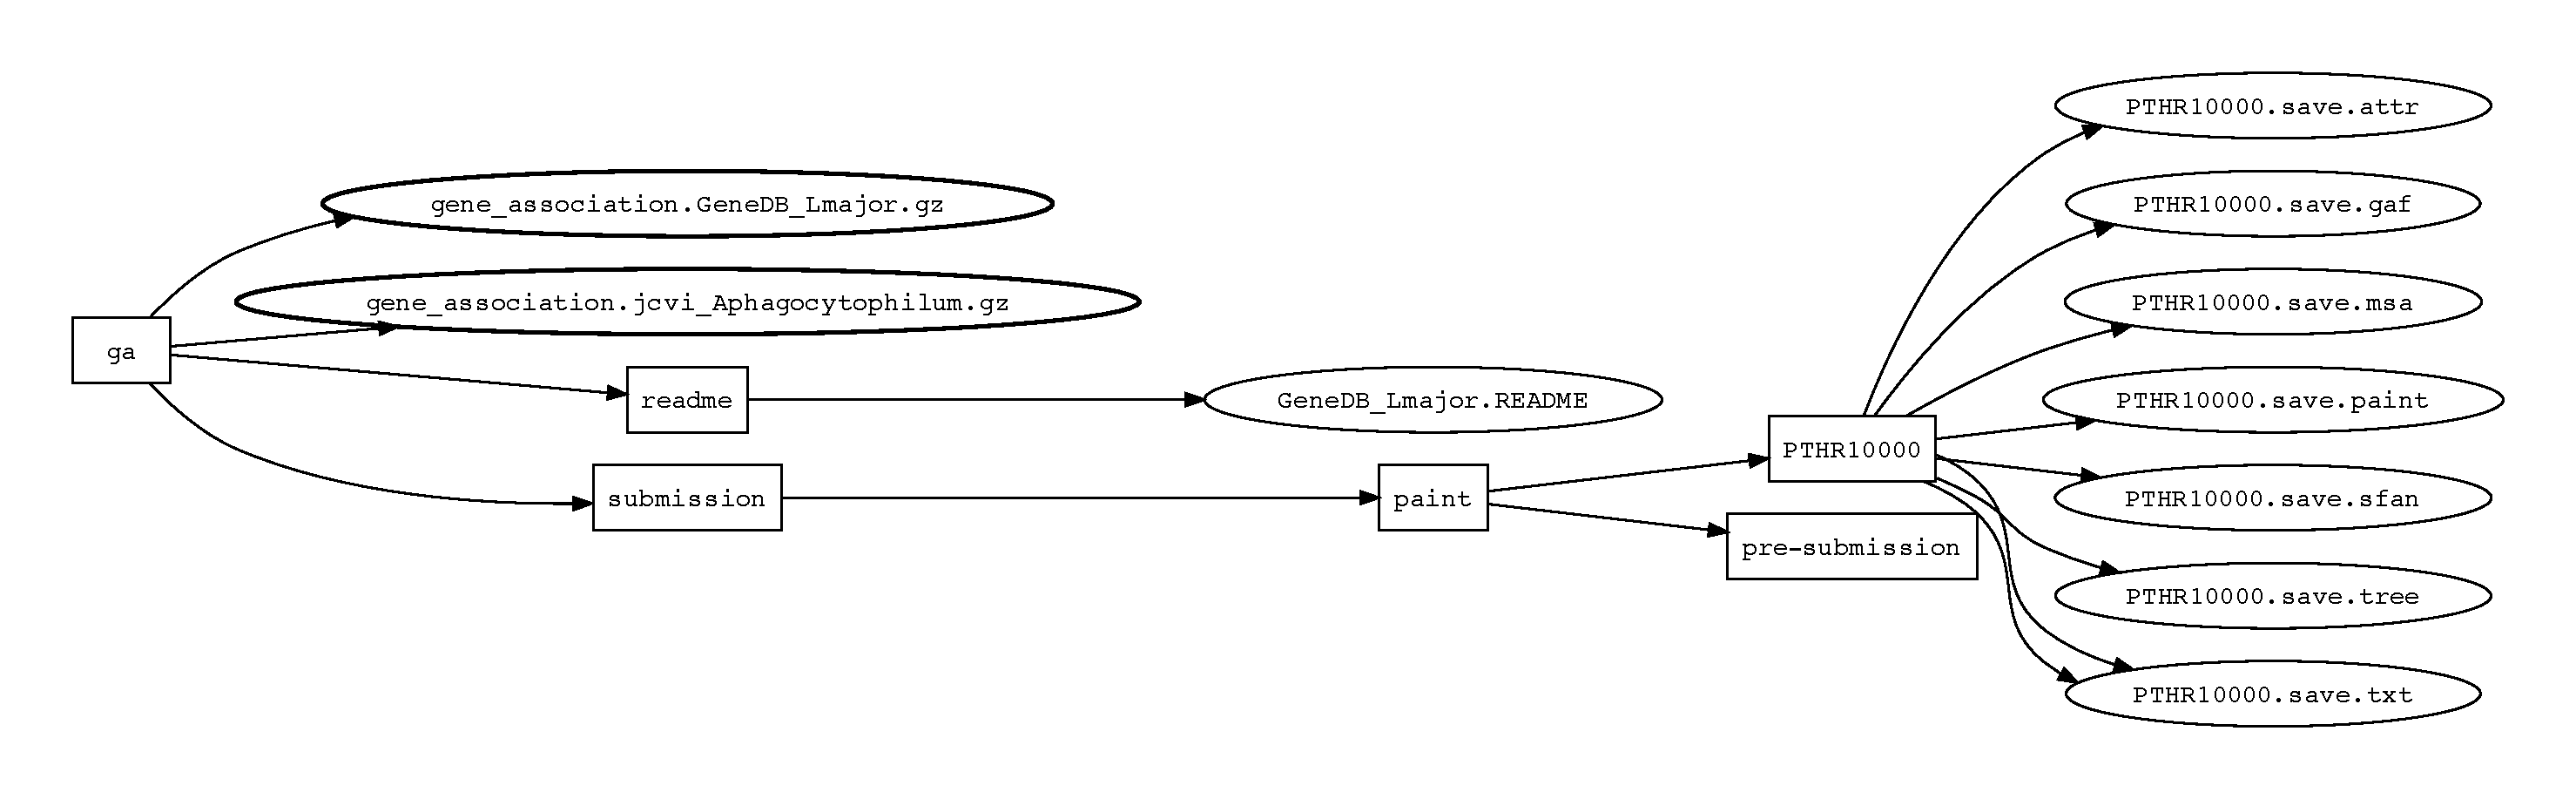
\includegraphics{ga.pdf}}
\end{center}
\caption{Graph showing structure of a small subset of the Gene Ontology \filestore, generated from 
  the description using \texttt{ForestGraph}}
\label{fig:ga}
\end{figure}


\newpage

\section{CVS.hs Description}

This section provides a generic description for CVS repositories.

\begin{code}
\textcolor{red}{-- PADS description of CVS file formats}
[pads| \kw{type} Repository_f = Line Pstringln

       \kw{data} Mode_t = Ext ":ext:" | Local ":local:" | Server ":server:" 

       \kw{data} Root_t = \{ cvs_mode :: Maybe Mode_t
                     , machine  :: Pstring ':', ':'
                     , path     :: Pstringln            
                     \}                                  
       \kw{type} Root_f = Line Root_t

       \kw{data} Dentry_t = \{ "D/"
                       , dirname :: Pstring '/'
                       , "////"
                       \}
\mbox{}
       \kw{data} Revision_t  = Version (Pint, '.', Pint) | Added '0' | Removed '-'
       \kw{data} TimeStamp_t = \{ ts       :: PstringSE (RE "[/+]")
                          , conflict :: Maybe ('+', Pstring '/') \}
\mbox{}
       \kw{type} Fentry_t = \{                                  "/"  
                       , filename   :: Pstring '/',       "/"
                       , revision   :: Revision_t,        "/"
                       , timestamp  :: TimeStamp_t,       "/"   
                       , options    :: Pstring '/',       "/"  
                       , tagdate    :: Pstringln
                       \}

       \kw{data} Entry_t   = Dir Dentry_t | File Fentry_t | NoDir 'D'
     
       \kw{type} Entries_f = [Line Entry_t] \kw{with} term Eof
|]
\end{code}
\begin{code}

\textcolor{red}{-- Auxiliary Haskell functions}
getEntries cvs = \kw{let} (Entries_f l) = entries cvs \kw{in} l
getDirName  d  = \kw{let} (Pstring s)   = dirname   d \kw{in} s
getFileName f  = \kw{let} (Pstring s)   = filename  f \kw{in} s
\mbox{}             
isDir entry  = \kw{case} entry \kw{of} {Dir _  -> True; otherwise -> False}
isFile entry = \kw{case} entry \kw{of} {File _ -> True; otherwise -> False}
\mbox{}                            

getDirs  cvs = map (\textbackslash(Dir d)  -> d) (filter isDir  (getEntries cvs))
getFiles cvs = map (\textbackslash(File f) -> f) (filter isFile (getEntries cvs))
\end{code}
\begin{code}

\textcolor{red}{-- FOREST description of CVS directory structure}
\textcolor{red}{-- Note that this description is recursive.}
\textcolor{red}{-- Note also that the collection of dirs and the 
-- collection of files are determined from information in the cvs 
-- directory.}
[forest| \kw{type} CVS_d = \kw{Directory}
              \{ repository \kw{is} "Repository" :: File Repository_f
              , root       \kw{is} "Root"       :: File Root_f
              , entries    \kw{is} "Entries"    :: File Entries_f
              \}
\mbox{}             
         \kw{type} CVS_Repository_d = Directory
             \{ cvs         \kw{is} "CVS"                 :: CVS_d
             , dirs        \kw{is} [ n \kw{as} <| getDirName  d |> :: CVS_Repository_d | d <- <| getDirs  cvs |> ]
             , files       \kw{is} [ <| getFileName f |> :: Text       | f <- <| getFiles cvs |> ]
             \} |]

\end{code}
\begin{code}
\textcolor{red}{-- Sample use of PADS and FOREST descriptions}
meta_dir     = "Examples/CVS"
entries_file = meta_dir ++ "/Entries"
doParseEntries = \kw{do} \{
 (rep, md)  <- parseFile entries_file
\}
\mbox{}             
doLoadCVS = \kw{do} \{
   (meta_rep, meta_md) <- cVS_d_load meta_dir
\}
\end{code}

\section{Universal.hs Description}

This section includes a universal data description.  This universal description
is used to drive some of our generic tools.

\begin{code}
\textcolor{red}{-- Universal Forest Directory Description}

[forest| 
  \kw{type} Universal_d = \kw{Directory}
     \{ ascii_files  \kw{is} [ f :: Text        | f <- \kw{matches} (GL "*"), <| get_kind  f_att == AsciiK     |> ]
     , binary_files \kw{is} [ b :: Binary      | b <- \kw{matches} (GL "*"), <| get_kind  b_att == BinaryK    |> ]
     , directories  \kw{is} [ d :: Universal_d | d <- \kw{matches} (GL "*"), <| get_kind  d_att == DirectoryK |> ]
     , symLinks     \kw{is} [ s :: SymLink     | s <- \kw{matches} (GL "*"), <| get_isSym s_att == True       |> ]
     \} 
|]
\end{code}
\begin{code}

\textcolor{red}{-- Use of Universal directory}
universal_dir = "Examples/data/universal"
doLoadUniverse = \kw{do} \{
 (rep, md) <-  universal_d_load  universal_dir
 \}
\end{code}


\end{document}




\fi

\end{document}

%%% Local Variables:
%%% mode: outline-minor
%%% End:

